\documentclass[12pt, a4paper, oneside]{book}   	% document style definition


\usepackage{hslu}                               % apply HSLU style
\usepackage{comment}                            % having comment sections \begin{comment} \end{comment}
\usepackage[utf8]{inputenc}						% charactere interpretation
\usepackage{amsmath}							% math package
\usepackage{amsfonts}							% font package for math symbols
\usepackage{amssymb}							% symbols package - definition of math symbols
\usepackage{listings}							% package for code representation

\usepackage{csquotes}       % Quotation support
\usepackage[style=apa,backend=biber]{biblatex}       % Bibliography, 
% todo: original template uses ieee3
\DeclareLanguageMapping{american}{american-apa}
\addbibresource{references.bib} % Bibliography file

\usepackage{graphicx}							% for inclusion of image
\setlength {\marginparwidth }{2cm}
\usepackage{todonotes}
\renewcommand{\todo}[1]{\textcolor{red}{TODO: #1}}
%\presetkeys{todonotes}{inline, textcolor=red, color=none, noinlinepar}{}

%\let\todoold\todo
%\newcommand{\todo}[1]{\textcolor{red}{TODO: #1}\todo[prepend, caption={TODO: #1}]{}}

%\renewcommand{\todo}[1]{\todo[inline]{\textcolor{red}{TODO: #1}}}
%\renewcommand{\todo}[1]{\todo{\textcolor{red}{TODO: #1}}}




\usepackage{booktabs}       % Better tables
\usepackage{caption}        % Better captions
\usepackage{subfig}								% to arrange figures next to each other
\usepackage{float}								% text style surrounding images
\usepackage{threeparttable}
\usepackage{tikz}								% used to place logos on title page
% \usepackage{gensymb}							% for special characters such as °
\usepackage{titlesec}
\usepackage{multirow}
\usepackage{siunitx}
\usepackage{tabularx}
\usepackage{tikzscale}
\usepackage{csvsimple}

\usepackage{appendix}

% PDF/A Compliance, todo: enable and remove hyperref usepackage afterwards
% \usepackage[a-1b]{pdfx}
% \catcode30=12

\usepackage{hyperref}
\hypersetup{hidelinks}

\newcommand{\linkchap}[1]{\hyperref[#1]{chapter~\ref{#1}~\nameref{#1}}}
\newcommand{\linkapp}[1]{\hyperref[#1]{appendix~\ref{#1}~\nameref{#1}}}

\usepackage[acronym]{glossaries}         				% package for glossary

\setcounter{tocdepth}{1}                        % hide subsections from TOC
\makenoidxglossaries
\newacronym{HSLU}{HSLU}{Lucerne University of Applied Sciences and Arts}
\newacronym[see={[Glossary:]{fitzpatrick-skin-type}}]{FST}{FST}{Fitzpatrick skin type\glsadd{fitzpatrick-skin-type}}
\newacronym{ML}{ML}{Machine Learning}
\newacronym{AI}{AI}{Artificial Intelligence}
\newacronym{FPR}{FPR}{false positive rate}
\newacronym{TPR}{TPR}{true positive rate}
                                % include acronyms.txt file
\newglossaryentry{fitzpatrick-skin-type}{
	name={Fitzpatrick skin type},
	plural={Fitzpatrick skin types},
	description={A skin classifier based on the skins' reaction to ultraviolet light, developed by dermatologist Dr. Thomas Fitzpatrick \autocite{Gottfrois2024}}
}
\newglossaryentry{JupyterNotebook}{
	name={Jupyter Notebook},
	description={Executable files, often used in ML to write Python code and add explanations in text form}
}
\newglossaryentry{gpuhub}{
	name={GPUhub},
	description={\gls{HSLU}’s server infrastructure for GPU-related computing. It provides isolated environments with JupyterLab access for developing and running \gls{ML} workflows}
}
\newglossaryentry{pediatric}{
	name={pediatric},
	description={A medical term for infants, children and adolescents \autocite{Farlex_nodate}}
}
\newglossaryentry{proxyVar}{
	name={proxy variable},
	plural={proxy variables},
	description={"one or more variables that encode the protected attribute with a substantial degree of accuracy" \autocite{Wang_2021}}
}
\newglossaryentry{teledermatology}{
	name={teledermatology},
	description={dermatological care from a distance, supported by modern technology \autocite{Pala_2020}}
}
\newglossaryentry{Fairlearn}{
	name=Fairlearn,
	description={A Python library for assessing and improving fairness in machine learning models. It supports various fairness metrics and mitigation techniques, especially for binary classification tasks \autocite{Fairlearn_nodate}}
}
\newglossaryentry{Equalized-Odds-Difference}{
	name={equalized odds difference},
	description={The absolute difference in true positive and false positive rates between subgroups, used as a group fairness metric \autocite{Fairlearn_nodate}}
}
\newglossaryentry{Equalized-Odds-Ratio}{
	name={equalized odds ratio},
	description={The ratio of true positive and false positive rates between subgroups, used as a group fairness metric \autocite{Fairlearn_nodate}}
}                                % include glossary.txt file
\graphicspath{{figures/}}						    % set path of graphics folder



% Format chapter titles without "Chapter X" prefix
\titleformat{\chapter}[hang]
{\normalfont\LARGE\bfseries}  % Style: Large bold text
{\thechapter}                 % Number format: Just the number
{1em}                         % Space between number and title
{}                            % Code before the title (empty)


% changed paragraph and subsection appearance
\setcounter{secnumdepth}{3}
\renewcommand{\paragraph}[1]{%
	\subsubsection*{#1}%
%	\addcontentsline{toc}{subsection}{#1}%
}


% mentioned in header
\newcommand{\tblWidthDescription}{\hsize=0.6\hsize\raggedright}
\newcommand{\tblWidthContext}{\hsize=0.2\hsize}


%improved basic functionality
\newcommand{\bolditalic}[1]{\textbf{\textit{{#1}}}}

%indicate citations
% Define a flag to track whether we're inside a raw citation block
\newif\ifrawcitationactive
\rawcitationactivefalse % Default: Not inside a raw citation block

% Define color commands with conditional checking
\newcommand{\rawcitationstart}{
	\color{purple}\rawcitationactivetrue
}
\newcommand{\rawcitationend}{
	\color{black}\rawcitationactivefalse
}

\newcommand{\rawcitationusedstart}{\color{violet}}
\newcommand{\rawcitationusedend}{%
	\ifrawcitationactive
	\color{purple}  % If inside rawcitation, reset to purple
	\else
	\color{black}  % Otherwise, reset to black
	\fi
}


% indicate info about criteria
\newcommand{\baaCriteria}[1]{\textcolor{blue}{#1}}


%----------------------------------------------------------------------------------------
%	DOCUMENT INFORMATION
%----------------------------------------------------------------------------------------
\author{Nadja Stadelmann}                       % author name
\city{Lucerne (Switzerland)}                    % author's place of origin
\title{Demographic Biases in\linebreak Dermatology Models}   % thesis title
\subtitle{\large \todo{subtitle}}               % thesis subtitle

\date{2025}                                     % the year when the thesis was written (for the titlepage)
\defensedate{\todo{adapt date} October 27th, 2024}                % the date of the private defense
\defencelocation{Lucerne}                       % location of defence
\extexpert{Dr. Jürg Schelldorfer}                         % name of external expert
\indpartner{Applied AI Research Lab}                       % name of industry partner

% jury, supervisor and dean are only relevant if acceptance sheet is enabled with the next line
% \acceptsheet
\jury{                                          % members of the jury
    \begin{itemize}
        \item Prof. Dr. Name Surname from Lucerne University of Applied Sciences and Arts, Switzerland (President of the Jury);
        \item Prof. Dr. Name Surname from Lucerne University of Applied Sciences and Arts, Switzerland (Thesis Supervisor);
        \item Prof. Dr. Name Surname from Lucerne University of Applied Sciences and Arts, Switzerland (External Expert).
    \end{itemize}
}

\supervisor{Dr. Ludovic Amruthalingam}             % name of supervisor
\dean{Prof. Dr. René Hüsler}                   % name of faculty dean

\acknowledgments{Thanks to my family, relatives and friends for all the support given to finish this thesis.
	\todo{add thanks and gratitude}
	Ludovic Amruthalingam
	Simone Lionetti - deputy Ludovic
	Pascal Baumann - LaTeX
	Philippe Gottfrois - information and work on PASSION project
	Proofreaders \todo{do you want to be mentioned with name or not?}
}


\begin{document}
	\english                                        % define thesis language: \german or \german
	\maketitle
	
	
	%----------------------------------------------------------------------------------------
	%	PREAMBLE
	%----------------------------------------------------------------------------------------
	\begin{abstractstyle}{\hsummary}
		\todo{Your abstract here.}
	    The content of your thesis in brief.
	\end{abstractstyle}
	
	\tableofcontents
	
	\listoftodos
	\todo{solve todos} 
	
	
	\todo{also solve todos in the code ;)} 
	
	
	\todo{also fix metadata entry!!!} 
	
	
	\todo{Portfolio DB für Referenzarbeiten anschauen}
	
	\todo{remove all \textbackslash rawcitationstart \textbackslash rawcitationend  \textbackslash baaCriteria}
	
	\todo{fix the weird line breaks}
	
	\todo{TEXT MISTAKES ensure fine-tuning ResNet-50, overview of instead of overview over, accuracy (you got all other versions of rr and cc); coma after e.g., point after vs., decision not desicion, decision-making not decision making ...}
	
	\todo{fix gls mentions in list of figures, it breaks how the glossary works}
	
	\todo{when you got to many pages: fix in order to - to, for the purpose of - For}
	
	
	\baaCriteria{Alle Fakten (fundiertes Wissen Dritter) sind korrekt zitiert. Es werden verschiedene Zitierweisen verwendet und teilweise mehrere Interpretationen gegenübergestellt. Der gemeinsam definierte Zitierstil im Text, in Abbildungen und Tabellen sowie im Literaturverzeichnis wird korrekt und durchgängig angewendet. Eigene Leistungen (sowie Bewertungen) und Fremdquellen sowie Recherchen sind klar unterscheidbar.} 
	
	
	\baaCriteria{Die erstellten Artefakte sind von sehr hoher Qualität. Das trifft u.a. auf Diagramme, Skizzen sowie Notationen (z.B. BPMN/UML) zu. Darstellungen sind einwandfrei, alle statistisch notwendigen Qualitätskriterien sind erfüllt. Beschriftungen etc. sind vorhanden, keine Einwände, Text und Bild stimmen beschreibend gut überein. Es wurden angemessene Dokumentationsmethoden und -arten korrekt verwendet. Vereinbarte Interview Transkripte, Beobachtungsprotokolle bzw. Zusammen-fassungen sind vorhanden. Daten, Ort, Kontext, Beschreibung, Zeilennummer, Verweise, Strukturen sind erkennbar, gut formatiert und korrekt mit dem Text/ der Analyse verknüpft. Alle Elemente und Themen sind im methodischen Teil/Text erklärt und verständlich, keine technischen oder strukturellen Einwände. Auch Zwischenanalysen, Zwischenschritte oder Gesamtauswertungen wurden durchgeführt, die Herkunft der Daten ist erkennbar und professionell aufbereitet.} 
	
	
	\baaCriteria{Der Schreibstil aller Dokumente entspricht hohen Standards und enthält keine Übertreibungen oder unbegründete Beurteilungen. Die Sprache ist aussagekräftig, prägnant und präzise. Die Fachterminologie ist konsistent, d.h. für gleiche Gegenstände und Themen werden immer die gleichen Begriffe verwendet. Der Sprachgebrauch ist durchgängig geschlechtergerecht, einheitlich und sachlich.}
	
	\listoffigures
	\listoftables
	% print list of acronyms and glossary
	\printnoidxglossaries
	
	\todo{fix citations in glossary}
	
	%----------------------------------------------------------------------------------------
	%	MAIN CONTENT
	%----------------------------------------------------------------------------------------
	\mainmatter
	
	% write or compose the main document here
	
	\chapter{Problem Statement}
		\baaCriteria{Welche Ziele, Fragestellungen werden mit dem Projekt verfolgt? Die Bedeutung, Auswirkung und Relevanz dieses Projektes für die unterschiedlichen Beteiligten soll aufgeführt werden. Typischerweise wird hier ein Verweis auf die Aufgabenstellung im Anhang gemacht.}
		
		In Sub-Saharan Africa dermatology treatment is inaccessible according to \textcite{Gottfrois2024}. There is fewer than one dermatologist available per one million people. Despite this, up to 80\% of the children and adolescents in the area are affected by skin conditions. \Gls{teledermatology} based on \gls{AI} promises to close this gap of specialists per case, for example by serving as a triage option. Potential patients could upload pictures to diagnostic dermatology \glspl{AI} which can indicate whether the person should indeed visit a dermatologist or promote other treatment options. However, current dermatology \glspl{AI} tend to fail to deliver accurate results for patients with highly pigmented skin tones. This is mainly due to demographic biases in existing \gls{AI} models. The models are trained on established datasets which mainly feature low pigmented skin. Therefore, the datasets lack representation of highly pigmented skin, leading to AI models which do not generalize to the population in Sub-Saharan Africa \autocite{Gottfrois2024}.
		
		These biases result in unequal access to treatment and especially affect underrepresented groups. Such biased results must be avoided, especially in AI models which impact life-changing decisions \autocite{Mehrabi_2021}.
		
		According to \textcite{Diaz2022}, demographic biases are especially important in dermatology. Demographic differences in patients influence the appearance of dermatological conditions. The differences in appearance can be developed depending on genetic factors, such as skin tone, age and sex \autocite{Diaz2022}. Research showed, that in patients with lower socio-economic status the disease progression is more advanced at time of diagnosis, which in turn can lead to different appearances for the same disease \autocite{BAD2021}. Since the AI models use pictures as the inputs and can only learn to diagnose diseases according to their appearances in the data, the factors which affects the disease appearances must be considered when creating an inclusive dataset.
		
		In order to overcome these issues, the PASSION research team founded the PASSION project. The projects vision is to make dermatology treatment accessible in Africa by enabling the AI-supported \gls{teledermatology} for triage by reducing the demographic biases in the dermatology AI models. For this bias mitigation, the researcher collected a dataset in Sub-Saharan Africa, focusing on patients with highly pigmented skin and the most common regional \gls{pediatric} skin conditions. The PASSION dataset is complementary to existing datasets and improves their diversity. With this dataset, the PASSION team trained a ResNet-50 model which was pretrained on ImageNet. This thesis refers to this trained model as the PASSION model. It should serve as a benchmark model to assess other dermatology models in regards of fairness \autocite{Gottfrois2024}. \todo{check sources, maybe, for the last sentence, the midterm protocol must be cited instead}
		
		So that the PASSION model can become an unbiased benchmark model, potential demographic biases in it must be reduced as far as possible. To reach this goal, demographic biases in the model as well as the limitation of the gathered dataset must be identified and mitigated. This thesis supports the PASSION team in this process. The main objective of the thesis is to assess the effectiveness of mitigation strategies to reduce demographic biases in context of PASSION.
		
		
		\begin{comment}
		\begin{enumerate}
			\item Identify demographic biases in dermatology AI models, using established fairness metrics.
			\item Identify mitigation strategies to minimize these biases.
			\item Assess the effectiveness of the mitigation strategies.
		\end{enumerate}
		It is important to identify the existent biases first, so that the mitigation strategies can be \todo{proceed here to reason why you chose those objectives}
		\end{comment}
		
	    \rawcitationstart
		\begin{itemize}
			\item With the advent of telemedicine, developing countries are learning newer ways of leveraging their information and communication technologies (ICTs) to play an increasingly
			vital role in the health care industry. Telemedicine is defined as a health care delivery mechanism where physicians and other medical personnel can examine patients remotely
			using information and telecommunication technologies (ICTs; Bashshur, Sanders, and Shannon, 1997). \autocite{Kifle_2024}
			\rawcitationusedstart
			\item AI systems can be used in many sensitive environments to make important and life-changing decisions; thus, it is crucial to ensure that these decisions do not reflect discriminatory behavior toward certain groups or populations \autocite{Mehrabi_2021}.
			\rawcitationusedend
			\item There are clear benefits to algorithmic decision-making; unlike people, machines do not become tired or bored [45, 119], and can take into account orders of magnitude more factors than people can. However, like people, algorithms are vulnerable to biases that render their decisions “unfair” [6, 121]. In the context of decision-making, fairness is \textit{the absence of any prejudice or favoritism toward an individual or group based on their inherent or acquired characteristics}. Thus, an unfair algorithm is one whose decisions are skewed toward a particular group of people. \autocite{Mehrabi_2021}.
			\item it is important for researchers and engineers to be concerned about the downstream applications and their potential harmful effects when modeling an algorithm or a system \autocite{Mehrabi_2021}.
			\item We should think responsibly, and recognize that the application of these tools, and their subsequent decisions affect peoples’ lives; therefore, considering fairness constraints is a crucial task while designing and engineering these types of sensitive tools \autocite{Mehrabi_2021}.
		\end{itemize}
		\rawcitationend
	
		\begin{comment}
			
		This thesis is part of the PASSION project. The PASSION research team identified that in Africa, dermatology treatment is not accessible. There is less than one dermatologist per one million citizens. In contrast, there is high demand for dermatology treatment, especially among children and adolescents. 80\% of the \gls{pediatric} population is affected. The goal of PASSION is to make dermatology treatment more accessible by using AI supported telemedicine for triage \autocite{Gottfrois2024}.
		
		For AI supported triage, demographic biases in existing dermatology models is a problem since the corresponding datasets lack diversity, especially regarding skin tones \autocite{Gottfrois2024}. This type of bias is important in dermatology, since different diseases present themselves differently depending on the skin-color \autocite{Diaz2022}. Further, skin diseases are more advanced or severe at diagnosis in patients with lower socioeconomic status \autocite{BAD2021}.
		
		PASSION tries to mitigate the demographic bias by providing a dataset of pigmented skin images of patients from Sub-Saharan Africa. The PASSION team focused on gathering data with \gls{FST} IV, V and VI. Further, the covered conditions represent up to 80\% of the conditions in the \gls{pediatric} population, the demographic group who is most affected by skin disease \autocite{Gottfrois2024}. \gls{HSLU}
		
		The PASSION dataset is complementary to the existing datasets and improves the diversity in a combined dataset. Within the dataset itself, there could potentially be further demographic biases, e.g. related to age or gender.

		\section{Objective}
			The goal of this research is to
			\begin{enumerate}
				\item Identify demographic biases in dermatology AI models, using established fairness metrics.
				\item Identify mitigation strategies to minimize these biases.
				\item Assess the effectiveness of the mitigation strategies.
			\end{enumerate}
			It is important to identify the existent biases first, so that the mitigation strategies can be \todo{proceed here to reason why you chose those objectives}
		\end{comment}
	
	\chapter{State of Research}
		\baaCriteria{Bezogen auf die eigenen Zielsetzungen und Fragestellungen soll aufgezeigt werden, wie andere dieses oder ähnliche Probleme gelöst haben. Worauf können Sie aufbauen, was müssen Sie neu angehen?	Wodurch unterscheidet sich Ihre Lösung von anderen Lösungen? Für wissenschaftlich orientierte Arbeiten sei hier explizit auf (Balzert, S. 66 ff) verwiesen.}
		\baaCriteria{Relevante, aktuelle und fundierte Fachliteratur wurde identifiziert, kritisch geprüft und verwendet. Die Begriffe der Fragestellung sind definiert und referenziert. Der gesamte Kontext ist verknüpft und eine Abgrenzung wurde vorgenommen. All dies ist in einer leicht verständlichen Struktur formuliert und überprüft.}
		
		This chapter provides a review of existing work in the field of bias mitigation in \gls{AI}. The main focus lies on a literature review of existing papers from other researchers in this area, highlighting the key findings which are connected to this thesis. Bias mitigation in \gls{AI} has already been investigated by different researchers, who crafted fitting mitigation methods \todo{citation?}. This thesis aims to assess those existing methods in the context of PASSION.
		
		Therefore, this chapter first presents an overview of the PASSION project based on the PASSION paper and dataset. Then, the general knowledge in the literature about existing biases, fairness metrics and mitigation methods is summarized. The review process was divided into two main contexts: \gls{ML} in general, and \gls{ML} in dermatology. This approach ensures that the technical and dermatological perspectives are considered when applying the knowledge to PASSION. The tables in this chapter indicate which points were found in which context. This is important, since what may be an issue in general might not be relevant for a specific use case or vice versa. For example, in theory, all age groups should be represented in datasets to account for demographic diversity. However, for car insurance, age representation is not important, because age does not affect how well a driver can drive \todo{either cite this example from the expert or find another example related to dermatology}.
		
		The various studies present different bias sources and suggest diverse methods to mitigate them. During the literature review, several biases and mitigation methods were identified that may be relevant to the PASSION project. Since it is not feasible to assess all of them during the duration of this thesis, the thesis focuses on those which are related to skin type, age and gender. The chosen methods are explained in \linkchap{chap:methodology}. The other items are passed to the PASSION research team as a list for further investigation. The list can be found in the appendix \todo{add link}.
		
		
		\todo{put the evaluation stuff in the execution / analysis section!!}
		
		
		\section{PASSION for Dermatology}
			This section provides an overview of the PASSION project regarding its medical scope and technical components.
			
			While the overall goal remains to improve the accessibility of dermatological care by building fair and inclusive AI systems, PASSION specifically addresses common \gls{pediatric} skin conditions in Sub-Saharan Africa. To create a dataset which represents patients with highly pigmented skin, they collected data from patients with \glspl{FST} III to VI. Based on this dataset, the PASSION team fine-tuned a ResNet-50 model using transfer learning. With the dataset and trained model, the researchers published data analysis scripts and initial insights on the model performance in a MICCAI \todo{add to glossary} publication \autocite{Gottfrois2024}.
			
			For the purpose of this thesis, it is essential to understand the dataset's metadata, the architecture and fine-tuning process of the PASSION model and which bias mitigation methods have already been applied. The dataset can influence which biases could arise in the model or rather which ones can be measured. The labels which should be predicted, and the model architecture give insight into the \gls{ML} task. All this information affects which mitigation methods are feasible to be used for the project. \todo{add sources}
			
			\subsection{PASSION Dataset}
				The PASSION dataset contains data from patients from four African countries in dermatology clinics. It contains 4901 images of 1653 dermatology cases with the corresponding demographic and clinical metadata. Each patient is represented by one record, with images linked to the record via filename. The images were captured with mobile phones to ensure that the training data complies with a \gls{teledermatology} setting regarding image quality \autocite{Gottfrois2024}.
				
			    A predefined 80/20 stratified train-test split at patient level ensures reproducibility and fair comparison, while preventing information leaking \autocite{Gottfrois2024}.
			    
			    Stratified splitting is a method to split  datasets while maintaining the original class distribution within the subsets. This is important for imbalanced datasets to maintain minority class representation  \autocite{Balde_2023}. \todo{add better source for the stratified data split (and the other stuff where medium was used)}.
				
				The metadata, as listed in \autoref{tab:PASSION_metadata}, includes demographic attributes such as \textit{age}, \textit{sex}, and \textit{\gls{FST}}. These are essential for identifying potential demographic biases lateron.	The labels \textit{impetig} and \textit{conditions\_PASSION} represent dermatology diagnosis as evaluated by dermatologists \autocite{Gottfrois2024}, and are the target variables the PASSION model learns to predict. Therefore, this \gls{ML} task is a multilabel classification problem. PASSION addresses this by training separate models for each label \autocite{Gottfrois2024}. The prediction of conditions\_PASSION is a multiclass classification task, while predicting impetig is a binary classification task. 
				
				\begin{table}[H]
					\centering
					\begin{tabularx}{\textwidth}{>{\hsize=.27\hsize}X>{\hsize=.27\hsize\raggedright}X>{\hsize=.46\hsize}X}
						\toprule
						\textbf{Metadata Attribute}       & \textbf{Data Type} & \textbf{Description}       \\ \midrule
						subject\_id          & string & Participant's unique identifier        \\
						country              & string & Country of data origin \\
						age                  & integer & Age of the participant in years       \\
						sex                  & m/f/o & Gender of the participant               \\
						fitzpatrick          & integer & \gls{FST}                \\
						body\_loc            & string (list; null-able, semicolon-separated) & Specifically affected body locations \\
						impetig              & 0/1  & Presence of impetigo (1=present), may occur alone or with other conditions, affects the treatment options for coexisting conditions        \\
						conditions\_PASSION  & Eczema, Scabies, Fungal, Others & Primary diagnosed skin condition \\
						\bottomrule
					\end{tabularx}
					\caption{PASSION dataset - metadata attributes and descriptions \autocite{Gottfrois2024}}
					\label{tab:PASSION_metadata}
				\end{table}
				
				The PASSION team also provides a set of \gls{JupyterNotebook}-based data analysis scripts. For example, one script analyses the correlation between the clinical conditions and location of the data collection. A full list of these scripts is included in \linkapp{app:PASSIONdataAnalysisScripts}. Additionally, the paper visualizes demographic analyzes related to age, sex and \gls{FST} as shown in \autoref{fig:PASSIONDistr}.
				
				
				\begin{figure}[H]
					\centering
					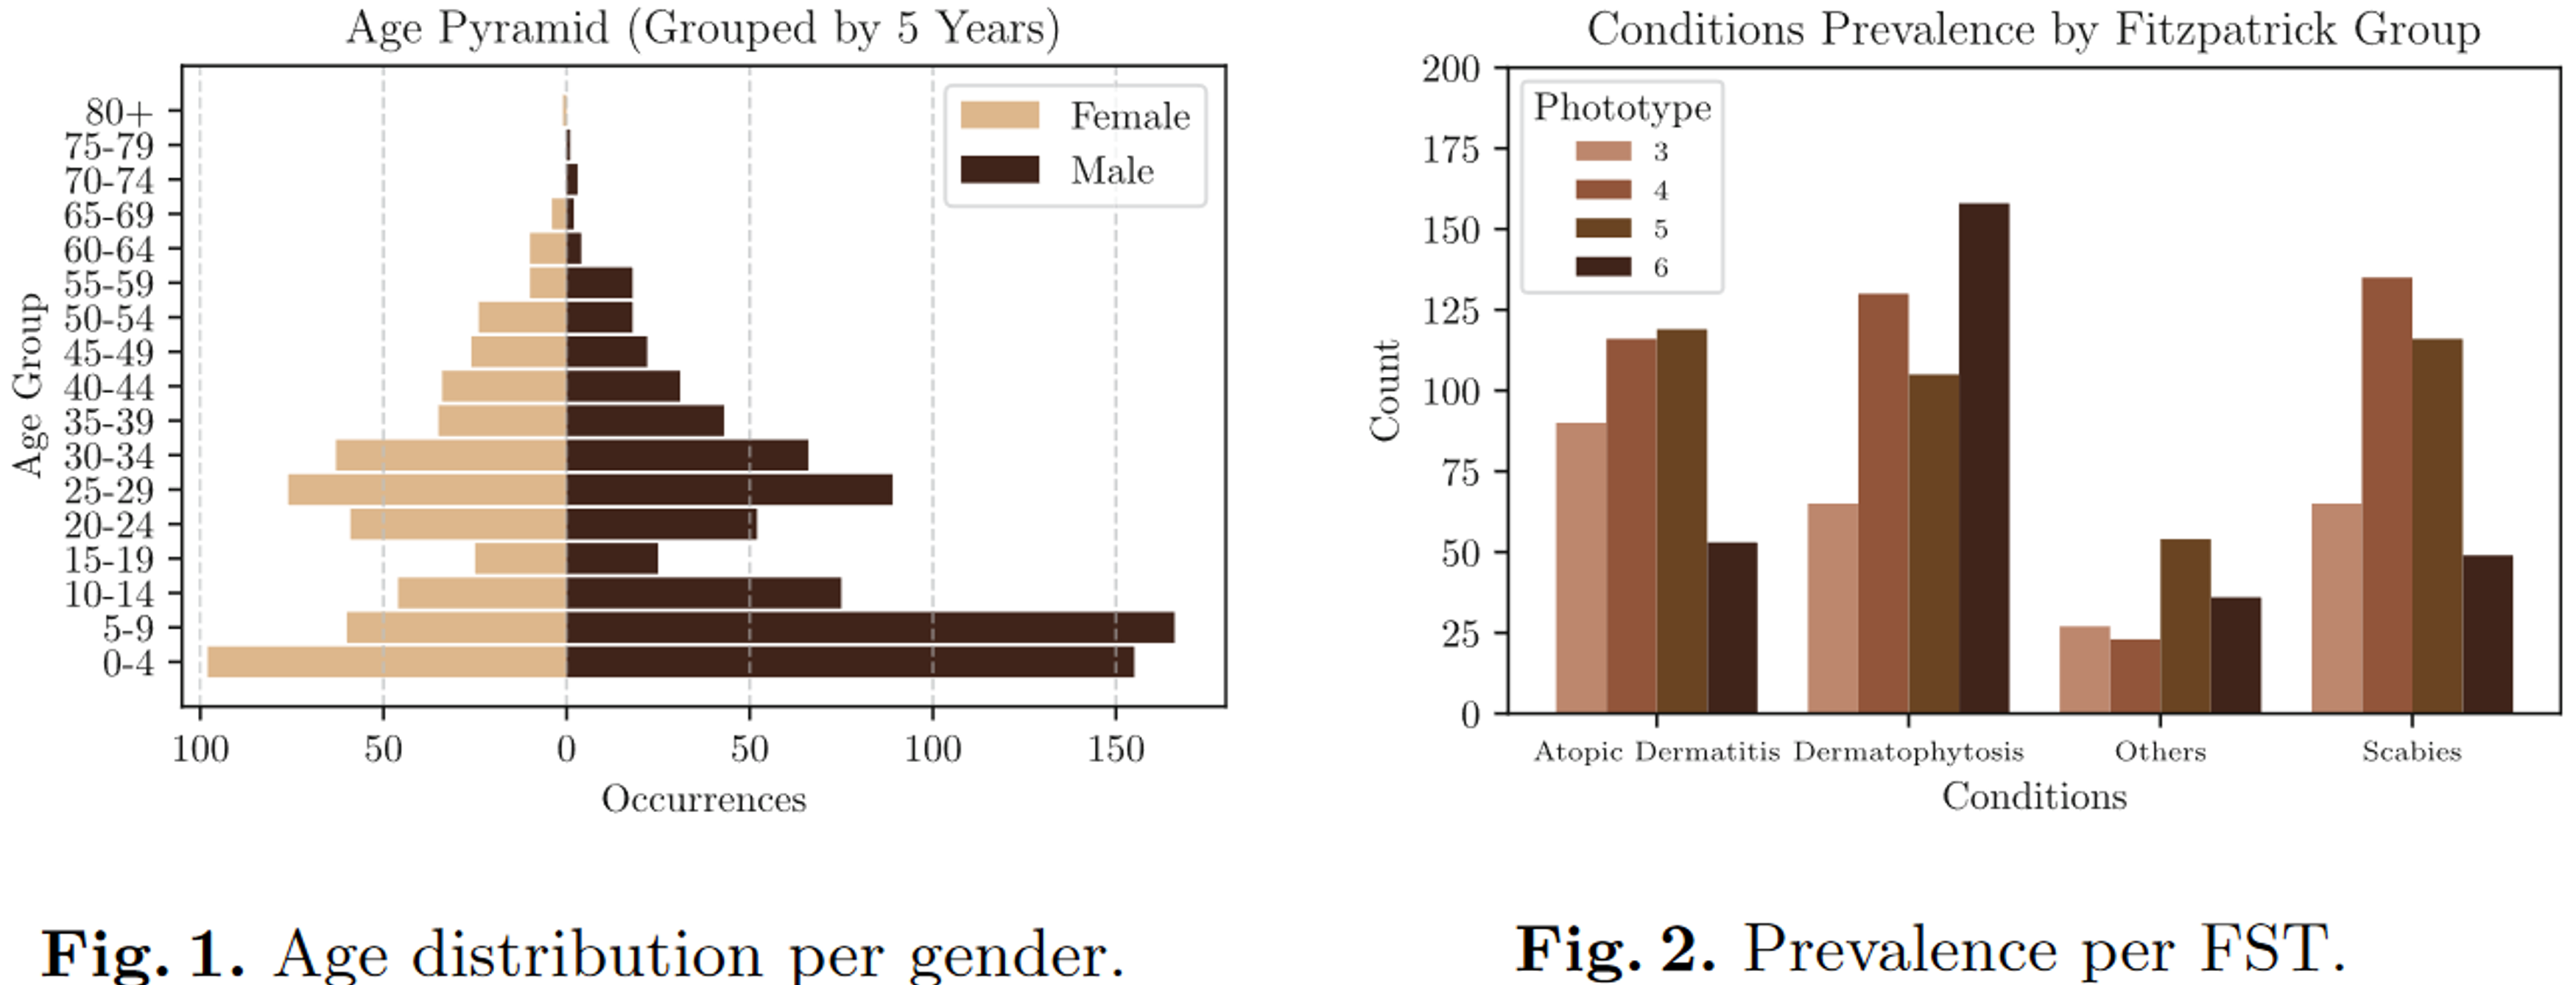
\includegraphics[width=0.9\textwidth]{figures/PASSIONDatasetDistribution.png}
					\caption{PASSION data distributions \autocite{Gottfrois2024}}
					\label{fig:PASSIONDistr}
				\end{figure}
				
				
				Due to the sensitivity of patient data, the dataset is confidential. Access to it can be requested via the project website: \href{https://passionderm.github.io/}{https://passionderm.github.io/} \autocite{Gottfrois2024}.
				
			\subsection{PASSION Model}
			  The model architecture is a ResNet-50 model which is pretrained on ImageNet. The model was fine-tuned by replacing the last fully connected classification layer with a dropout layer with a 0.3 dropout rate followed by batch normalization. The class activation is done by a single linear layer. To minimize the weighted cross-entropy loss, Adam optimization is used. For improved generalization and to avoid overfitting, data augmentations were applied. The methods used were random resizing, cropping, flipping, and rotating \textcite{Gottfrois2024}. \todo{add individual citations for ResNet-50, ImageNet, Adam optimization, weighted cross-entropy loss}.
			  
			  \todo{add information regarding how many folds are there, how is the data split, ...}
			  			
			\subsection{PASSION Experiments}
			  The PASSION team conducted various experiments to evaluate the classifiers on the test set with the following schemes \autocite{Gottfrois2024}:
			  \begin{itemize}
			  	\item Performance for skin condition prediction
			  	\item Performance for impetigo detection
			  	\item Generalization from two centers to a wider population (test set contains data from the known centers and one unknown center)
			  	\item Generalization from different age groups (test set contains data from the known age groups and one unknown)
			  	\item Subject level analysis over the predictions of multiple pictures, using majority voting
			  \end{itemize}
			  
			  The code for those experiments is available in the PASSION evaluation GitHub repo. This repo can serve as a starting point, since reproducing the results helps to verify that the provided setup works the same on my side. Also, they can be used as examples for further experiments. \todo{mention which ones I really used why for the thesis and move the others to the appendix}
			  
			  The paper indicates lower performance when evaluating the model on a subject level (performance per case/patient) rather than a sample level (performance per image). The authors emphasize the importance of assessing classifier performance on both levels for completeness \autocite{Gottfrois2024}. Therefore, the subject level performance should also be considered during this thesis.
			  \todo{challenge this to be tested again in the outlook bc of the inproper metadata linkage}
	
	
		\subsection{Limitations}
				\todo{maybe move to execution phase}
				\todo{write in more details}
			   - multiple executions showed inconsistent results for the different group evaluations on the same model checkpoint. It turned out that the metadata linkage did not work consistently. I resolved the issue was resolved by providing the image name in the data loader and link the metadata directly from the source file instead of using the indexes. probably related to different shuffling between data loader and metadata loader
		
			\begin{comment}
				\todo{probably remove this}
		
			\subsection{Telemedicine \todo{is this chapter needed?}}
				\rawcitationstart
				\begin{itemize}
					\item Teledermatology. Telemedicine may be one of the first fields to embrace AI, driven by demand for services, the necessity of collecting fit-for-purpose high-quality images, and the availability of existing technology (Xiong et al., 2019). Face-to-face diagnostic accuracy exceeds that of teledermatology (Finnane et al., 2017); however, inequalities surrounding access to dermatological care persist. Teledermatology has the potential to increase access by facilitating referrals and offering convenience and decreased wait times (Finnane et al., 2017), as well as providing diagnostic support at the time of case review. For teledermatology cases, the accuracy of a DL classifier (0.67) matched dermatologists’ (0.63) and was higher than primary care physicians’ (0.45) for 26 skin conditions (Liu et al., 2019b). AI may be integrated into smartphone apps to photograph skin lesions, collect relevant clinical information, and generate a referral if appropriate. Many smartphones already support on-device DL with Google’s TensorFlow Lite (TensorFlow, 2020) or Apple’s Core\gls{ML} (Apple Inc, 2020), preserving privacy by keeping health information on the device. A systematic review found nine studies that evaluated six algorithm-based smartphone apps and concluded that evidence of diagnostic accuracy was poor and does not support current implementation, despite two apps having obtained the CE marking; no apps are Food and Drug Administration approved (Freeman et al., 2020). AI may also assist in automatic tracking and monitoring of skin lesions; although preliminary results are promising, existing studies used small datasets with little description, and there is no established standard metric of change (Navarro et al., 2019). Further study hinges on the prospective collection of large datasets. \autocite{Young_2020}
					\item \autocite{Tsetsi_2017} on smartphone / internet access divide between populations
					\item https://www.tandfonline.com/doi/full/10.1080/08870446.2019.1579330 on how open people are to use AI
				\end{itemize}
				\rawcitationend
			\end{comment}
		
		
		\section{Bias}
			This chapter provides an overview of biases and related demographic characteristics mentioned in \gls{ML}- and dermatology-related research. It also explains their relevance for PASSION.
			
			Algorithmic decisions made by \gls{AI} systems can directly affect peoples' lives. In healthcare applications such as PASSION, these decisions are especially sensitive, as they influence diagnoses and treatment outcomes. Diverse studies have shown that \gls{AI} application's decisions can hold biases that affect underrepresented groups. This leads to unfair or even harmful consequences. Therefore, it is essential for \gls{AI} engineers to identify, address, and mitigate such biases in order to develop fair applications. This requires an understanding of what bias is in general, which concrete biases exist, and where they originate \autocite{Mehrabi_2021}.
			
			
			\begin{comment}
			\rawcitationusedstart
			\begin{itemize}
				\item Bias in facial recognition systems [128] and recommender systems [140] have also been largely studied and evaluated and in many cases shown to be discriminative towards certain populations and subgroups. In order to be able to address the bias issue in these applications, it is important for us to know where these biases are coming from and what we can do to prevent them.\autocite{Mehrabi_2021}.
				\item We should think responsibly, and recognize that the application of these tools, and their subsequent decisions affect peoples’ lives; therefore, considering fairness constraints is a crucial task while designing and engineering these types of sensitive tools \autocite{Mehrabi_2021}.
			\end{itemize}
			\rawcitationusedend
			
			\end{comment}
		
			\subsection{Definition of Bias in \gls{ML}}
		    In the context of \gls{ML}, bias can be defined as \textit{a systematic error that causes a model or estimator to consistently deviate from the true value or relationship} \autocite{Delgado-Rodriguez_2004, Taylor_2023}. In practice, this often results in models that make less accurate predictions for specific subgroups within the population \todo{cite this}.
		    			    
		  	\todo{make sure the following is cited correctly}
			
			\subsection{Demographic Biases in the Context of Dermatology} \label{chap:demographicBiasesDermatology}
			Biases in dermatology in general can lead to unequal outcomes for different groups, which can result in unfair outcomes for certain groups. Demographic biases are particularly relevant in the context of dermatology \glspl{AI}, as they can cause differences in diagnostic accuracy and treatment outcomes among different demographic (sub-)groups.
			From the literature review, three main ways have been identified in which demographic differences may introduce bias in dermatology \gls{ML} models:
			\todo{cite all that, from presentation}
			
			\begin{itemize}
				\item \textbf{Disease Presentation}. \textit{Skin type} affects how diseases appear on the skin. As Gottfrois notes, "any condition linked to inflammation is less visible if the skin is more pigmented" \todo{cite mail from philippe}. This directly influences training and evaluating image-based \gls{ML} models like those used in PASSION. For example, a model trained predominantly on images with low pigmented skin may perform poorly on images of highly pigmented skin.
				
				\item \textbf{Disease Prevalence}. Factors such as \textit{age} and \textit{sex} do not tend to affect disease presentation, but they can influence disease prevalence \todo{cite mail from philippe}. Also, \textit{geographic location} can influence the prevalence of skin conditions (e.g., tropical vs. dry climates) \todo{add source}. Therefore, these factors could introduce bias if certain conditions are underrepresented in the dataset due to demographic imbalances. \todo{consider adding smt like the car driver example here, indicating that it is not necessarily a problem due to the same disease presentation}
				
				\item \textbf{Access to Healthcare}. \textit{Socioeconomic status} or \textit{geographic location} can also introduce bias. Research shows that patients with lower socioeconomic status are often diagnosed at later stages of the disease, which may alter the visual presentation of the disease. If such cases are missing in training data, the model may fail to recognize them, leading to misdiagnosis. \todo{add example for geographic location?}.
			\end{itemize}
			
			
			To build a robust and fair \gls{ML} model, it is essential to identify and address biases linked to such protected characteristics \autocite{Mehrabi2022}.
			\todo{check that there is no duplication between PASSION dataset feature description and here}
			\todo{probably remove}
			Due to time constraints, this thesis focuses on three protected characteristics: skin type, age, and sex. These were selected based on their presence in the PASSION dataset and their influence on dermatological diagnosis and disease prevalence. Other potentially relevant features, such as geographic location and socioeconomic status, should be evaluated in future work by the PASSION team.
			
			
			\begin{comment}
				\todo{if citing is an issue: check the comment}
						
				It captures three distinct pathways through which demographic differences can introduce bias in dermatological machine learning systems:
				
				Disease Presentation — covers how diseases manifest differently on various skin types, directly affecting the visual input to image-based models.
				Disease Prevalence — focuses on who is more likely to have certain conditions, which affects label distribution in the dataset.
				Access to Healthcare — reflects when and how people enter the medical system, influencing data collection quality and representativeness.
				
				Each of these groups addresses a different layer of the data generation and learning process:
				
				Input variability (visual features),
				Target/label imbalance (class representation),
				Data collection bias (who gets diagnosed and when).
				
				This structure is also supported in literature on medical \gls{AI} fairness (e.g., in works by Obermeyer et al. or Adamson & Smith).
			\end{comment}
			
			\subsection{Types of Biases and Their Relevance for PASSION}
			The literature describes numerous types of bias. Over 60 were identified during this research. These factors were grouped into categories to provide an overview, and their relevance to the PASSION context was assessed.
			
			Among them, \textit{sampling biases} and \textit{representation biases} are particularly relevant, as they relate directly to the inclusion or exclusion of demographic subgroups in the dataset. For example, \textit{ascertainment bias}, a subtype of sampling bias, occurs when parts of the target population are unintentionally excluded. A common example is healthcare studies conducted in public hospitals only, which excludes patients from higher socioeconomic backgrounds who visit private clinics. This skews the data and can lead to incorrect conclusions, such as overestimating disease prevalence in specific groups.
			
			Other relevant categories include \textit{medical biases} and \textit{imaging biases}, especially in the teledermatology setting of PASSION. These include clinical labeling errors, variations in image quality or lighting conditions which lead to bias.
			
			
			This thesis focuses on the most relevant bias types. An extensive list is provided in \linkapp{app:listOfBiases} and will be shared with the PASSION team for further evaluation.
			
			\todo{add the 5-10 most important biases here}
			
			\subsection{Sensitive Features}
			Research has identified sensitive features that are particularly prone to bias. These features have already caused biases in existing \gls{AI} applications and should therefore be carefully evaluated during model development \autocite{Mehrabi_2021}.
			
			\autoref{tab:biases_features} summarizes sensitive features mentioned in the literature. The categorization in the table was done based on the research described in \autoref{chap:demographicBiasesDermatology}. For completeness, the table also contains sensitive demographic features which appear unrelated to dermatology according based on current research.
			
			\begin{comment}
			\todo{check what to do with those additional features:}
			Other important features according to (\autocite{Montoya_2025} 13):
			lesion type, anatomical location of lesion, img characteristics such as source, imaging techniques, resolution, real vs. artificially generated
			
			In addition to demographic factors, domain-specific variables such as lesion type, anatomical location, and image characteristics (e.g., imaging technique, resolution, device source, or whether an image is real vs. artificially generated) can also influence model behaviour \autocite{Montoya_2025}. These features are important considerations for dataset curation and model evaluation in dermatology-focused applications like PASSION.
			\end{comment}
			
			
			\begin{table}[H]
				\centering
				\begin{threeparttable}
					\begin{tabularx}{\textwidth}{>{\tblWidthDescription}X|>{\tblWidthContext}X|>{\tblWidthContext}X}
						\toprule
						\textbf{Bias-Sensitive Features} & \multicolumn{2}{c}{\textbf{Mentioned in Context of}} \\
						& \textbf{\gls{ML}} & \textbf{Dermatology} \\
						%\midrule
						\multicolumn{3}{l}{\textbf{Related to Disease Presentation}} \\
						Skin Type & X\tnote{1,2,7} & X\tnote{12,13}\\
						Skin Undertones & & X\tnote{13} \\
						Socio-Economic Status & X\tnote{6} & X\tnote{12} \\
						Geographic Location \todo{double check this!} & X\tnote{1,3} & \\
						
						\multicolumn{3}{l}{\bolditalic{Related to Disease Prevalence}} \\
						Age & X\tnote{7,11} &  X\tnote{13} \\
						Gender/Sex & X\tnote{1,2,7,8,9,10,11} & X\tnote{13} \\
						Gender and Skin Type Subgroups & X\tnote{1,2} & \\
						
						\multicolumn{3}{l}{\bolditalic{Related to Access to Healthcare}} \\
						Geographic Location & X\tnote{1,3} & \\
						Socio-Economic Status & X\tnote{6} & X\tnote{12} \\
						
						\multicolumn{3}{l}{\bolditalic{Relation to Dermatology to be Checked}} \\
						Ethnicity/Race & X\tnote{1,2,4,5,6,7,11}&  X\tnote{12,13} \\
						Disabilities & X\tnote{7,11} & \\
						
						\multicolumn{3}{l}{\bolditalic{Unrelated to Dermatology}} \\
						Familial status & X\tnote{7} & \\
						Marital status & X\tnote{7,11} & \\
						Nationality/National origin & X\tnote{7,11} & \\
						Recipient of public assistance & X\tnote{7} & \\
						Religion & X\tnote{7,11} & \\
						\bottomrule
					\end{tabularx}
					\begin{tablenotes}
						\footnotesize
						\begin{minipage}{0.33\textwidth}\raggedright
							\item[1] \autocite{Mehrabi_2021}
							\item[2] \autocite{M24_Buolamwini_2018}
							\item[3] \autocite{M142_Shankar_2017}
							\item[4] \autocite{M98_Manrai_2016}
							\item[5] \autocite{M54_Fry_2017}
						\end{minipage}%
						\begin{minipage}{0.33\textwidth}\raggedright
							\item[6] \autocite{M150_Vickers_2014}
							\item[7] \autocite{M30_Chen_2019}
							\item[8] \autocite{M167_Zhao_2017}
							\item[9] \autocite{M20_Bolukbasi_2016}
							\item[10] \autocite{M168_Zhao_2018}
						\end{minipage}%
						\begin{minipage}{0.33\textwidth}\raggedright
							\item[11] \autocite{M62_Hajian_2013}
							\item[12] \autocite{Young_2020}
							\item[13] \autocite{Montoya_2025}
						\end{minipage}%
					\end{tablenotes}
				\end{threeparttable}
				\caption{Commonly used features which often are affected by biases}
				\label{tab:biases_features}
			\end{table}
			
			
			\begin{comment}
			\todo{decide which table to use, more or less extensive citations?}
			
			\begin{table}[H]
				\centering
				\begin{threeparttable}
					\begin{tabularx}{\textwidth}{>{\tblWidthDescription}X|>{\tblWidthContext}X|>{\tblWidthContext}X}
						\toprule
						\textbf{Bias-Sensitive Features} & \multicolumn{2}{c}{\textbf{Mentioned in Context of}} \\
						& \textbf{\gls{ML}} & \textbf{Dermatology} \\
						%\midrule
						\multicolumn{3}{l}{\textbf{Dermatology Related Features}} \\
						Skin Type & X\tnote{1,3} & X\tnote{5,6}\\
						Skin Undertones & & X\tnote{6} \\
						
						\multicolumn{3}{l}{\textbf{Demographic Features}} \\						\multicolumn{3}{l}{\bolditalic{Relevant for Skin Disease Detection}} \\
						Age & X\tnote{3,4} &  X\tnote{6} \\
						Gender/Sex & X\tnote{1,3,4} & X\tnote{6} \\
						Gender and Skin Type Subgroups & X\tnote{1} & \\
						Ethnicity/Race & X\tnote{1,2,3,4}&  X\tnote{5,6} \\
						
						\multicolumn{3}{l}{\bolditalic{Potentially Relevant for Skin Disease Detection}} \\
						Geographic Location & X\tnote{1} & \\
						Socio-Economic Status & X\tnote{2} & X\tnote{5} \\
						Disabilities & X\tnote{3,4} & \\
						
						\multicolumn{3}{l}{\bolditalic{Not Relevant for Skin Disease Detection}} \\
						Familial status & X\tnote{3} & \\
						Marital status & X\tnote{3,4} & \\
						Nationality/National origin & X\tnote{3,4} & \\
						Recipient of public assistance & X\tnote{3} & \\
						Religion & X\tnote{3,4} & \\
						\bottomrule
					\end{tabularx}
					\begin{tablenotes}
						\footnotesize
						\begin{minipage}{0.30\textwidth}\raggedright
							\item[1] \autocite{Mehrabi_2021}
							\item[2] \autocite{M150_Vickers_2014}
						\end{minipage}%
						\begin{minipage}{0.40\textwidth}\raggedright
							\item[3] \autocite{M30_Chen_2019}
							\item[4] \autocite{M62_Hajian_2013}
						\end{minipage}%
						\begin{minipage}{0.30\textwidth}\raggedright
							\item[5] \autocite{Young_2020}
							\item[6] \autocite{Montoya_2025}
						\end{minipage}%
					\end{tablenotes}
				\end{threeparttable}
				\caption{Features which often hold biases}
				\label{tab:biases_sensitive_features}
			\end{table}
			\end{comment}
			
		\section{Fairness Metrics}
		This chapter introduces the concept of fairness in \gls{ML}, as fairness is a way to detect whether and what biases exist in a model. As there is no universally accepted definition of fairness, various fairness metrics have been proposed in the literature, each based on different assumptions and goals.
		This chapter focuses on those fairness metrics which are able to evaluate demographic fairness and are applicable to the dermatology context of PASSION.	
		Those are mainly \textit{equalized odds} by \textcite{M63_Hardt_2016} and \textit{subgroup fairness} by \textcite{M79_Kearns_2018}.
		
		
		\subsection{Definition of Fairness in \gls{ML}}
		
		In research, there is currently no common agreement regarding a fairness definition in \gls{ML}. Broadly, fairness \textit{is the absence of bias towards individuals or groups in a decision-making context}. To assess how fair \gls{AI} models are, multiple fairness metrics have been proposed in the literature, each reflecting different interpretations of fairness. The choice of metric largely depends on the specific use case of the application \autocite{Mehrabi_2021}.
		
		\subsection{Fairness Metrics}
		
			\textcite{Mehrabi_2021} summarized the fairness metrics and grouped them into the categories group fairness, subgroup fairness and individual fairness, depending on the main mechanics of the metrics. They are listed in \autoref{tab:fairness_definitions}.
			
			\todo{evtl in anhang wenn es zu viele Seiten werden}
		
			\begin{table}[H]
			\centering
			\begin{threeparttable}
				\begin{tabularx}{\textwidth}{>{\tblWidthDescription}X|>{\tblWidthContext}X|>{\tblWidthContext}X}
					\toprule
					\textbf{Fairness Definitions} & \multicolumn{2}{c}{\textbf{Mentioned in Context of}} \\
					& \textbf{\gls{ML}} & \textbf{Dermatology} \\
					%	\midrule
					\multicolumn{3}{l}{\textbf{Group Fairness}} \\ 
					Conditional Statistical Parity    & X &   \\
					Demographic/Statistical Parity  & X & \\
					Equal Opportunity& X &   \\
					Treatment Equality & X &   \\
					Test Fairness         & X &   \\
					Equalized Odds     & X &   \\
					%	\midrule
					\multicolumn{3}{l}{\textbf{Subgroup Fairness}} \\ 
					Subgroup Fairness    & X &   \\
					%\midrule
					\multicolumn{3}{l}{\textbf{Individual Fairness}} \\ 
					Counterfactual Fairness     & X &   \\
					Fairness Through Awareness     & X &   \\
					Fairness Through Unawareness        & X &   \\
					%\midrule
					\multicolumn{3}{l}{\textbf{Not Categorized}} \\ 
					Fairness in Relational Domains& X &   \\
					\bottomrule
				\end{tabularx}
			\end{threeparttable}
			\caption{Fairness definitions based on \textcite{Mehrabi_2021}}
			\label{tab:fairness_definitions}
		\end{table}
		
		In the context of PASSION, the fairness metrics which consider both true positives and false positives are particularly relevant. A \textit{true positive} indicates that a disease was detected correctly, while a \textit{false positive} corresponds to a diagnosis of a disease that is not actually present. Including false positives helps to identify cases where individuals from certain demographic groups may be unfairly more likely to receive unjustified diagnoses. This has also been indicated by \textcite{Sabato_2024}.
		
		From the listed group fairness metrics, there is only one that considers true and false positives, which should therefore be used for the evaluation of PASSION. It is equalized odds, as introduced by \textcite{M63_Hardt_2016}: \newline
		"\textit{A predictor $\hat{Y}$ satisfies equalized odds with respect to protected attribute $A$ and outcome $Y$, if $\hat{Y}$ and $A$ are independent conditional on $Y$. \newline
		\(
		P(\hat{Y} = 1 \mid A = 0, Y = y) = P(\hat{Y} = 1 \mid A = 1, Y = y), \quad \forall y \in \{0, 1\}
		\)"} \todo{add formula list} \newline
		In other words, the probability of predicting a positive outcome should be the same across protected and unprotected groups, given the true label $Y$. This ensures that both \gls{TPR} and \gls{FPR} are equal across different demographic groups. If these rates are the same, like in the example of \autoref{fig:eqOdds}, the model satisfies equalized odds, and fairness is achieved. Since equalized odds compares conditional probability distributions across groups, it is a group fairness metrics.
		
		\begin{figure}[H]
			\centering
			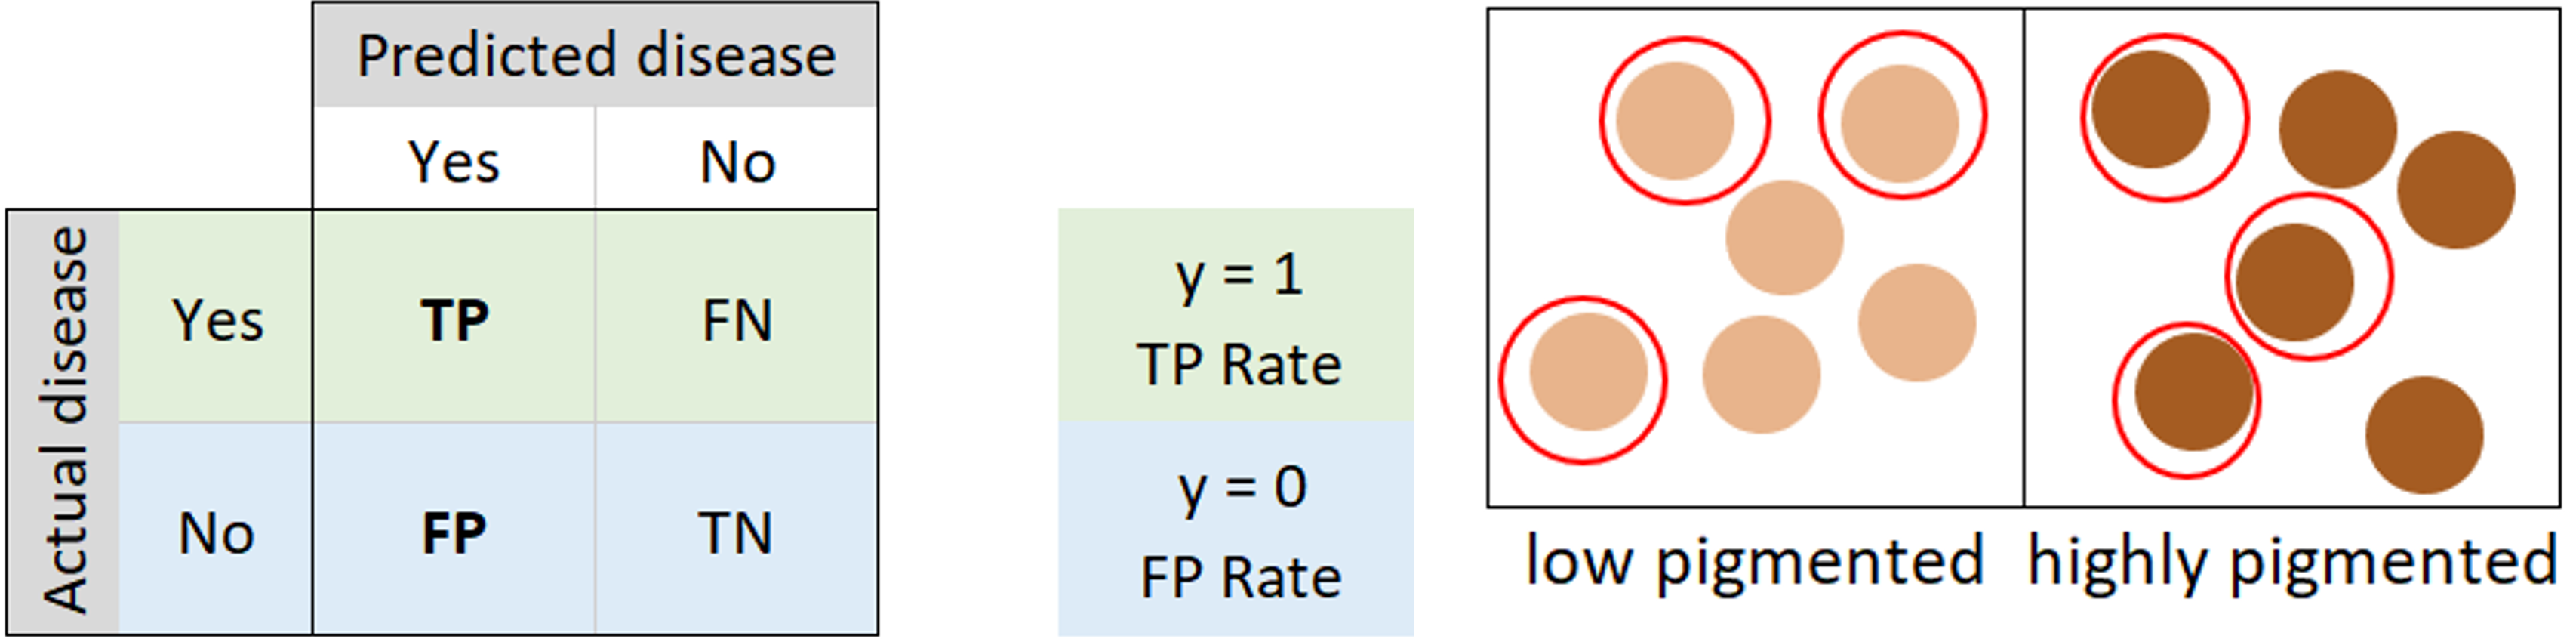
\includegraphics[width=0.9\textwidth]{figures/EqualizedOddsIllustration.png}
			\caption{Equalized odds mechanics, inspired by \autocite{M80_Kearns_2019}.}
			\label{fig:eqOdds}
		\end{figure}
		
		Given the specific dermatology use case in the context of PASSION, it is not clear whether individual fairness metrics would be feasible to use. Certain metrics propose to change attributes. This approach is not feasible for the skin type which is passed on to the model implicitly through the picture. Therefore, this thesis focuses on the group fairness metrics for now.
		
		The mechanics of the other fairness metrics are described broadly in \linkapp{app:fairnessMetrics}.
		
		\subsection{Limitations of Group Fairness}
		
		Despite its usefulness, equalized odds and similar group fairness metrics have limitations. These metrics can hide inequalities that exist within more specific subgroups. For example, a model might appear fair when assessed across broad groups such as age or skin type (\autoref{fig:eqOdds}) but still exhibit substantial disparities within subgroups, such as older individuals with darker skin tones (\autoref{fig:eqOddsLimits}) \autocite{M79_Kearns_2018,M80_Kearns_2019}.
		
		\begin{figure}[H]
			\centering
			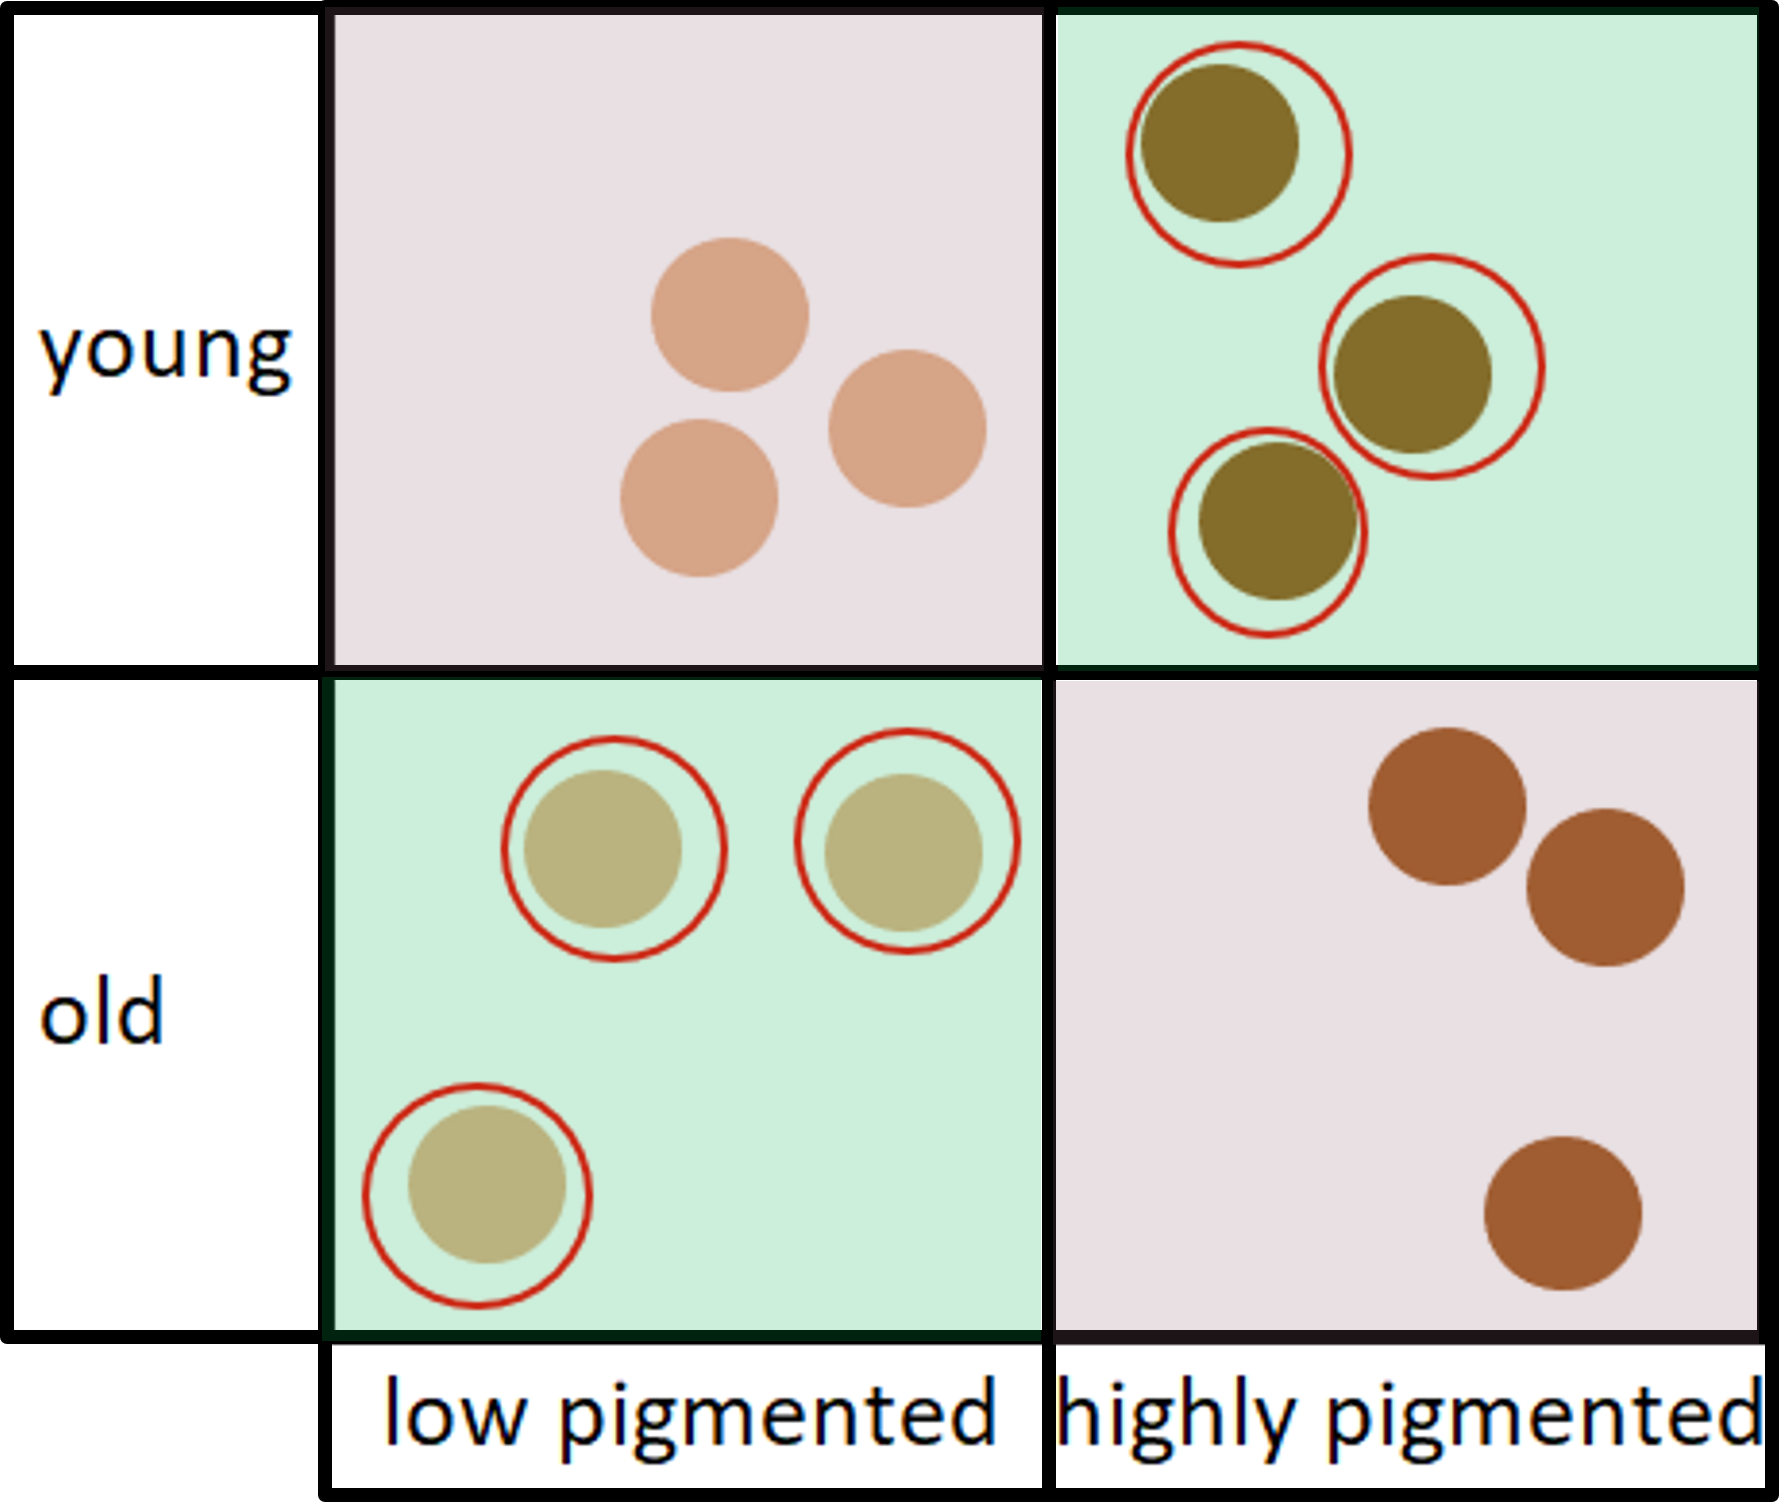
\includegraphics[width=0.5\textwidth]{figures/EqualizedOddsSubgroupsIssueIllustration.png}
			\caption{Equalized odds violations on subgroups, inspired by \autocite{M80_Kearns_2019}.}
			\label{fig:eqOddsLimits}
		\end{figure}
		
		To address this issue, subgroup fairness metrics have been proposed. These extend group fairness metrics by explicitly evaluating fairness across subgroups. This ensures that fairness assessments do not overlook hidden biases that could affect smaller populations \autocite{M79_Kearns_2018,M80_Kearns_2019}.
		
		Given the demographic focus of this study and the composition of the PASSION dataset, subgroup fairness is particularly important. Therefore, this thesis aims to incorporate equalized odds on subgroups as a core metric for evaluation.
		
		
		\subsection{Limitations of Fairness Evaluation in Multiclass Settings with Equalized Odds}
		Fairness metrics such as equalized odds are originally defined for binary classification problems, typically considering binary labels and binary demographic groups. As a result, fairness libraries like AI Fairness 360 and Fairlearn offer implementations of these fairness metrics only for binary classification tasks \todo{cite relevant sources} \todo{explain fairness libraries and add the individual ones to the glossar}. To evaluate fairness in multiclass settings using these libraries, certain considerations are required. This chapter introduces the two key challenges, handling multiclass labels and multiple subgroups.		
		
		\subsubsection{Multiclass Labels}
		In binary settings, fairness can be evaluated through simple comparisons of false positive and false negative rates. However, in multiclass classification, fairness must account for the full structure of the confusion matrix. \textcite{Sabato_2024} generalizes equalized odds to multiclass classification by defining:
		\textit{"For each \( y, z \in \mathcal{Y} \), the value of \( \mathbb{P}[\hat{Y} = z \mid Y = y, G = g] \) is the same for all \( g \in \mathcal{G} \)."}
		
		In practice, this means the entire confusion matrix must be equal across groups to satisfy strict multiclass fairness under equalized odds \autocite{Sabato_2024}. The similar approach is purposed by \textcite{Putzel_2022}.
		
		More relaxed versions of multiclass equalized odds have also been proposed in the literature. However, researchers argue that such relaxations may not be suitable in all contexts, especially when different types of errors carry different consequences \autocites{Sabato_2024}{Putzel_2022}.
		
		For instance, when the type of misclassification matters, equality of error rates is essential to ensure fairness, as noted by \textcite{Putzel_2022}. Furthermore, as \textcite{Sabato_2024} explicitly states, a fair classifier in healthcare should avoid differences in diagnosis errors for specific diseases across subgroups, since misdiagnoses can lead to different treatment outcomes. Therefore, in PASSION, the strict version of the multiclass equalized odds should be preferred.
		
		\subsubsection{Non-Binary Sensitive Features}
		There can also be non-binary sensitive features leading to multiple subgroups. The original definition of equalized odds does not account for this complexity. To generalize fairness evaluation to such settings, a one-vs-rest strategy can be applied. In this approach, each group is individually compared against the rest of the population \autocite{Nezami_2024}.
		
		
			
		\section{Mitigation Methods}
			 \todo{still to be written}
			 
			 \begin{comment}
			 see text from bias chapter - Further, \gls{AI} engineers need to know what prevention methods are available to reduce the biases \autocite{Mehrabi_2021}.
			 
			 
			
			
		\section{Extensive Sources}
			\subsection{Mitigation Methods Overview}
				\todo{write definitions of pre-in and post-processing, see Methods for fair machine learning below [43, 11, 14]}


				\todo{add stratified split}
				\todo{double check and futher improve groups}
				\begin{table}[H]
				\centering
				\begin{threeparttable}
						\begin{tabularx}{\textwidth}{>{\tblWidthDescription}X|>{\tblWidthContext}X|>{\tblWidthContext}X}
						\toprule
						\textbf{Mitigation Methods - Unbiasing Data (Pre-Processing)} & \multicolumn{2}{c}{\textbf{Mentioned in Context of}} \\
						& \textbf{\gls{ML}} & \textbf{Dermatology} \\
						\multicolumn{3}{l}{\textbf{Documentation and Transparency}} \\
						Good Practices while using Data & X\tnote{1,2,3} &   \\
						Datasheets as supporting document for dataset creation method, characteristics, motivations and skews & X\tnote{1,2,3} &   \\
						Datasheets as supporting document for model method, characteristics, motivations and skews & X\tnote{1,4} &   \\
						Dataset (Nutrition) Labels & X\tnote{1,5,6} & X\tnote{18, \todo{add spec source}}   \\
						
						\multicolumn{3}{l}{\textbf{Communication and Reporting}} \\
						Messaging & X\tnote{1,12} &   \\
						
						\multicolumn{3}{l}{\textbf{Bias Detection and Evaluation}} \\
						Test for Simpson's Paradox \todo{Discribe Simpson's Paradox} & X\tnote{1,7,8,9} &   \\
						Detect Direct Discrimination with Causal Models and Graphs & X\tnote{1,10} &   \\					
						Out-of-Distribution Detection in Dermatology Using Input Perturbation and Subset Scanning & & X\tnote{19} \\
						Check confidence interval and p-curve analysis instead of p-value & & X\tnote{17} \\
						 
						\multicolumn{3}{l}{\textbf{Study Design}} \\ 
						Allocation concealment and blinding & & X\tnote{17} \\
						Preventing Direct and Indirect Discrimination & X\tnote{1,11} &   \\
						
						\multicolumn{3}{l}{\textbf{Data Gathering}} \\ 
						Data Collection from diverse sources (incl. primary care clinics) & X\tnote{18} & \\
						Robust standards for external validation & X\tnote{18} & \\
						Preferential Sampling & X\tnote{1,13,14} &   \\
						Geographical Diversity and Inclusion for Dataset creation & X\tnote{16} & \\
						Balanced Representation accross skin tones and genders & & X\tnote{19} \\
						Disparate Impact Removal & X\tnote{1,15} &   \\
						
						\multicolumn{3}{l}{\textbf{Labeling}} \\ 
						Multidimensional Scale for Skin Tones & & X\tnote{19} \\
						
						
						\multicolumn{3}{l}{\textbf{Data Availability and Open Science}} \\ 
						Publish Datasets accessible for the public & & X\tnote{18, \todo{add source}} \\						
						
						\bottomrule
					\end{tabularx}
					\begin{tablenotes}
						\footnotesize
						\begin{minipage}{0.33\textwidth}\raggedright
							\item[1] \autocite{Mehrabi_2021}
							\item[2] \autocite{M13_}
							\item[3] \autocite{M55_}
							\item[4] \autocite{M110_}
							\item[5] \autocite{M66_}
							\item[6] \autocite{M66Successor_}
						\end{minipage}%
						\begin{minipage}{0.33\textwidth}\raggedright
							\item[7] \autocite{M81_}
							\item[8] \autocite{M3_}
							\item[9] \autocite{M4_}
							\item[10] \autocite{M163_}
							\item[11] \autocite{M62_Hajian_2013}
							\item[12] \autocite{M74_}
						\end{minipage}%
						\begin{minipage}{0.33\textwidth}\raggedright
							\item[13] \autocite{M75_}
							\item[14] \autocite{M76_}
							\item[15] \autocite{M51_}
							\item[16] \autocite{M142_Shankar_2017}
							\item[17] \autocite{Chakraborty_2024}
							\item[18] \autocite{Young_2020}
							\item[19] \autocite{Montoya_2025}
						\end{minipage}%
					\end{tablenotes}
				\end{threeparttable}
				\caption{Mitigation Methods - Unbiasing Data - Mentioned in Contextual Research, grouped like in \textcite{Mehrabi_2021}, the author cannot guarantee for completeness}
				\label{tab:mitigation_methods_unbiasing_data}
			\end{table}
				
				
			\begin{table}[H]
				\centering
				\begin{threeparttable}
					\begin{tabularx}{\textwidth}{>{\tblWidthDescription}X|>{\tblWidthContext}X|>{\tblWidthContext}X}
						\toprule
						\textbf{Mitigation Methods - Fair Classification} & \multicolumn{2}{c}{\textbf{Mentioned in Context of}} \\
						& \textbf{\gls{ML}} & \textbf{Dermatology} \\
						%	\midrule
						
						\multicolumn{3}{l}{\textbf{Satisfy Fairness Definitions}} \\ 
						Satisfy Subgroup Fairness  \todo{unclear if \tnote{*} in \tnote{3} as well, or if \tnote{2} also handles \tnote{*}} & X\tnote{1,2} &   \\
						Satisfy Equality of Opportunity\tnote{*} & X\tnote{1,3,6} & \\					
						Satisfy Equalized Odds\tnote{*} & X\tnote{1,3} &   \\
						Disparate Treatment\tnote{**} & X\tnote{1,4,5} &  \\
						Disparate Impact\tnote{**} & X\tnote{1,4,5} &  \\
						\todo{find out exact method} & X\tnote{1,7} &  \\
						\todo{find out exact method} & X\tnote{1,8} &  \\
						\todo{find out exact method} & X\tnote{1,9} &  \\
						\todo{find out exact method} & X\tnote{1,10} &  \\
						
						\multicolumn{3}{l}{\textbf{Satisfy Fairness and Stability Under Distribution Shifts}} \\ 
						\todo{find out exact method} & X\tnote{1,11} &  \\
						
						\multicolumn{3}{l}{\textbf{Fair Representation Learning (Pre/In-processing)}} \\ 
						Representation Learning by Disentanglement & X\tnote{1,2} &   \\
						Variational Fair Autoencoder & X\tnote{1,3,15} &   \\
						VAE without adversarial training & X\tnote{1,4} &   \\
						Adversial Learning with FairGAN & X\tnote{1,16} &   \\
						Removing correlation between protected and unprotected features with a geometric solution & X\tnote{1,17} &   \\
						
						\multicolumn{3}{l}{\textbf{Algorithmic Adaptions for Fairness}} \\ 
						Modified Discrimination-Free Naive Bayes Classifier & X\tnote{1,12} &  \\
						
						\multicolumn{3}{l}{\textbf{Fairness-Aware \gls{ML} Frameworks}} \\ 
						Fairness-Aware Classification Framework & X\tnote{1,13} &  \\
						Fairness Constraints in Multitask Learning (MTL) Framework & X\tnote{1,14} &  \\
						Decoupled Classification System with Transfer Learning & X\tnote{1,15} &  \\
						
						\multicolumn{3}{l}{\textbf{Preferential Data Selection and Representation}} \\ 
						Wasserstein Distance Measure for Dependence Mitigation & X\tnote{1,16} &  \\
						Preferential Sampling (PS) for Discrimination-Free Training Data & X\tnote{1,17} &  \\
						
						\multicolumn{3}{l}{\textbf{Model Interpretability}} \\ 
						Post-Processing with Attention Mechanism & X\tnote{1,18} &  \\
						Use Brier Score and Response Rate Accuracy & & X\tnote{19, \todo{add clear source}} \\
						some more methods \todo{describe} & & X\tnote{19} \\
						\bottomrule
					\end{tabularx}
					\begin{tablenotes}
						\footnotesize
						\begin{minipage}{0.33\textwidth}\raggedright
							\item[*] possible to satisfy together
							\item[**] possible to satisfy together
							\item[1] \autocite{Mehrabi_2021}
							\item[2] \autocite{M147_}
							\item[3] \autocite{M63_Hardt_2016}
							\item[4] \autocite{M2_}
							\item[5] \autocite{M159_}
						\end{minipage}%
						\begin{minipage}{0.33\textwidth}\raggedright
							\item[6] \autocite{M154_}
							\item[7] \autocite{M57_}
							\item[8] \autocite{M78_}
							\item[9] \autocite{M85_}
							\item[10] \autocite{M106_}
							\item[11] \autocite{M69_}
							\item[12] \autocite{M25_}
						\end{minipage}%
						\begin{minipage}{0.33\textwidth}\raggedright
							\item[13] \autocite{M155_}
							\item[14] \autocite{M12_}
							\item[15] \autocite{M49_}
							\item[16] \autocite{M73_}
							\item[17] \autocite{M75_}
							\item[18] \autocite{M102_}
							\item[19] \autocite{Young_2020}
						\end{minipage}%
					\end{tablenotes}
				\end{threeparttable}
				\caption{Mitigation Methods - Fair Classification - Mentioned in Contextual Research, grouped like in \textcite{Mehrabi_2021}, the author cannot guarantee for completeness}
				\label{tab:mitigation_methods_fair_classification}
			\end{table}
			
			\todo{check categorization}
			\begin{table}[H]
				\centering
				\begin{threeparttable}
					\begin{tabularx}{\textwidth}{>{\tblWidthDescription}X|>{\tblWidthContext}X|>{\tblWidthContext}X}
						\toprule
						\textbf{Mitigation Methods - not so relevant for us} & \multicolumn{2}{c}{\textbf{Mentioned in Context of}} \\
						& \textbf{\gls{ML}} & \textbf{Dermatology} \\
						%	\midrule
						\multicolumn{3}{l}{\textbf{Fair NLP}} \\ 
						Fair Word-Embedding & X\tnote{1,5,6,7} &   \\
						Train-Time Data Augmentation & X\tnote{1,8} &   \\
						Test-Time Neutralization & X\tnote{1,8} &   \\
						
						%	\midrule	
						\multicolumn{3}{l}{\textbf{Fair Regression (In-processing)}} \\ 
						Price of Fairness (POF) & X\tnote{1,10} & \\
						XY \todo{check this} and bounded group loss & X\tnote{1,11} & \\
						Decision Tree for Disparate Impact and Treatment & X\tnote{1,12} & \\
						
						%	\midrule
						\multicolumn{3}{l}{\textbf{Structured Prediction (In-processing)}} \\ 
						Reducing Bias Amplification (RBA) as calibration algorithm & X\tnote{1,13} & \\
						
						%	\midrule
						\multicolumn{3}{l}{\textbf{Principal Component Analysis (PCA) (In-processing)}} \\ 
						Fair PCA & X\tnote{1,14} & \\
						
						\multicolumn{3}{l}{\textbf{Graph-Based Fairness Methods}} \\ 
						Community Detection / Graph Embedding  \todo{how to proceed with this} & X\tnote{} & \\
						
						\multicolumn{3}{l}{\textbf{Causal Fairness and Disparate Learning}} \\ 
						Disparate Learning Processes (DLP) & X\tnote{1,9} &   \\
						Causal Approach to Fairness \todo{how to proceed with this} & X\tnote{\todo{add clear source}}  & \\
						Disregard path in causal graph which result in sensitive attributes affecting decision outcome & X\tnote{1} &   \\
						
						%	\midrule
						\multicolumn{3}{l}{\textbf{Removing Sensitive Attributes}} \\ 
						Disregard sensitive attributes in effect on decision-making & X\tnote{1} &   \\						
						\bottomrule
					\end{tabularx}
					\begin{tablenotes}
						\footnotesize
						\begin{minipage}{0.33\textwidth}\raggedright
							\item[1] \autocite{Mehrabi_2021}
							\item[2] \autocite{M42_}
							\item[3] \autocite{M97_}
							\item[4] \autocite{M112_}
							\item[5] \autocite{M20_Bolukbasi_2016}
							\item[6] \autocite{M58_}
						\end{minipage}%
						\begin{minipage}{0.33\textwidth}\raggedright
							\item[7] \autocite{M169_}
							\item[8] \autocite{M166_}
							\item[9] \autocite{M94_}
							\item[10] \autocite{M14_}
							\item[11] \autocite{M1_}
							\item[12] \autocite{M2_}
						\end{minipage}%
						\begin{minipage}{0.33\textwidth}\raggedright
							\item[13] \autocite{M167_Zhao_2017}
							\item[14] \autocite{M137_}
							\item[15] \autocite{M5_}
							\item[16] \autocite{M90_}
							\item[17] \autocite{M65_}
						\end{minipage}%
					\end{tablenotes}
				\end{threeparttable}
				\caption{Mitigation Methods - Others - Mentioned in Contextual Research, grouped like in \textcite{Mehrabi_2021}, the author cannot guarantee for completeness}
				\label{tab:mitigation_methods_others}
			\end{table}
			
			\todo{mention also the IBM AI Fairness 360 toolkit [11] and that authors evaluated their work in benchmark datasets [65], [72], [158], [159]}
			
			
			
			\todo{draft for presentation}
			satisfy Equalized Odds / Subgroup fairness
			highlight allocation concealment and blinding and data collection from diverse sources and Preferential Sampling
			\subsection{Mitigation Methods Overview}
			\begin{table}[H]
				\centering
				\begin{threeparttable}
					\begin{tabularx}{\textwidth}{>{\tblWidthDescription}X|>{\tblWidthContext}X|>{\tblWidthContext}X}
						\toprule
						\textbf{Mitigation Methods} & \multicolumn{2}{c}{\textbf{Mentioned in Context of}} \\
						& \textbf{\gls{ML}} & \textbf{Dermatology} \\
						\multicolumn{3}{l}{\bolditalic{Unbiasing Data}} \\
						Documentation and Transparency & X\tnote{1} & X\tnote{3} \\
						Bias Detection and Evaluation & X\tnote{1} & X\tnote{2,4} \\ % simpsons paradoxon, subset scanning, input pertubation
						Study Design & X\tnote{1} & X\tnote{2} \\ % allocation concealment and blinding, preventing direct and indirect discrimination
						Data Gathering & X\tnote{1} & X\tnote{3,4} \\ % data collection from diverse sources, robuster standards, 
						Data Availability and Open Science &  & X\tnote{3} \\
					    Removing Sensitive Attributes & X\tnote{1} &  \\
						\multicolumn{3}{l}{\bolditalic{Fair Classification}} \\
						Satisfy Fairness Definitions & X\tnote{1} &  \\ % satisfy Equalized Odds / Subgroup fairness
						Satisfy Fairness and Stability Under Distribution Shifts & X\tnote{1} & \\
						Fair Representation Learning & X\tnote{1} & \\
						Fairness-Aware \gls{ML} Frameworks & X\tnote{1} & \\
						Preferential Data Selection and Representation & X\tnote{1} & \\
						Model Interpretability & X\tnote{1} & X\tnote{3} \\
						\multicolumn{3}{l}{\bolditalic{For Other \gls{ML} Algorithm Types}} \\
						Fair NLP & X\tnote{1} &  \\
						Fair Regression & X\tnote{1} &  \\
						Structured Prediction & X\tnote{1} &  \\
						Fair Principal Component Analysis & X\tnote{1} &  \\
						Graph-Based Fairness Methods & X\tnote{1} &  \\
						Causal Fairness and Disparate Learning & X\tnote{1} &  \\
						\bottomrule
					\end{tabularx}
					\begin{tablenotes}
						\footnotesize
						\begin{minipage}{0.33\textwidth}\raggedright
							\item[1] \autocite{Mehrabi_2021}
							\item[2] \autocite{Chakraborty_2024}
						\end{minipage}%
						\begin{minipage}{0.33\textwidth}\raggedright
							\item[3] \autocite{Young_2020}
						\end{minipage}%
						\begin{minipage}{0.33\textwidth}\raggedright
							\item[4] \autocite{Montoya_2025}
						\end{minipage}%
					\end{tablenotes}
				\end{threeparttable}
				\caption{Mitigation Methods - Draft}
				\label{tab:mitigation_methods_unbiasing_data_praesi}
			\end{table}
			
			\todo{check categorization}
			\begin{table}[H]
				\centering
				\begin{threeparttable}
					\begin{tabularx}{\textwidth}{>{\tblWidthDescription}X|>{\tblWidthContext}X|>{\tblWidthContext}X}
						\toprule
						\textbf{Mitigation Methods - not so relevant for us} & \multicolumn{2}{c}{\textbf{Mentioned in Context of}} \\
						& \textbf{\gls{ML}} & \textbf{Dermatology} \\
						%	\midrule
						\multicolumn{3}{l}{\textbf{Fair NLP}} \\ 
						Fair Word-Embedding & X\tnote{1,5,6,7} &   \\
						Train-Time Data Augmentation & X\tnote{1,8} &   \\
						Test-Time Neutralization & X\tnote{1,8} &   \\
						
						%	\midrule	
						\multicolumn{3}{l}{\textbf{Fair Regression (In-processing)}} \\ 
						Price of Fairness (POF) & X\tnote{1,10} & \\
						XY \todo{check this} and bounded group loss & X\tnote{1,11} & \\
						Decision Tree for Disparate Impact and Treatment & X\tnote{1,12} & \\
						
						%	\midrule
						\multicolumn{3}{l}{\textbf{Structured Prediction (In-processing)}} \\ 
						Reducing Bias Amplification (RBA) as calibration algorithm & X\tnote{1,13} & \\
						
						%	\midrule
						\multicolumn{3}{l}{\textbf{Principal Component Analysis (PCA) (In-processing)}} \\ 
						Fair PCA & X\tnote{1,14} & \\
						
						\multicolumn{3}{l}{\textbf{Graph-Based Fairness Methods}} \\ 
						Community Detection / Graph Embedding  \todo{how to proceed with this} & X\tnote{} & \\
						
						\multicolumn{3}{l}{\textbf{Causal Fairness and Disparate Learning}} \\ 
						Disparate Learning Processes (DLP) & X\tnote{1,9} &   \\
						Causal Approach to Fairness \todo{how to proceed with this} & X\tnote{\todo{add clear source}}  & \\
						Disregard path in causal graph which result in sensitive attributes affecting decision outcome & X\tnote{1} &   \\
						
						%	\midrule
						\multicolumn{3}{l}{\textbf{Removing Sensitive Attributes}} \\ 
						Disregard sensitive attributes in effect on decision-making & X\tnote{1} &   \\						
						\bottomrule
					\end{tabularx}
					\begin{tablenotes}
						\footnotesize
						\begin{minipage}{0.33\textwidth}\raggedright
							\item[1] \autocite{Mehrabi_2021}
							\item[2] \autocite{M42_}
							\item[3] \autocite{M97_}
							\item[4] \autocite{M112_}
							\item[5] \autocite{M20_Bolukbasi_2016}
							\item[6] \autocite{M58_}
						\end{minipage}%
						\begin{minipage}{0.33\textwidth}\raggedright
							\item[7] \autocite{M169_}
							\item[8] \autocite{M166_}
							\item[9] \autocite{M94_}
							\item[10] \autocite{M14_}
							\item[11] \autocite{M1_}
							\item[12] \autocite{M2_}
						\end{minipage}%
						\begin{minipage}{0.33\textwidth}\raggedright
							\item[13] \autocite{M167_Zhao_2017}
							\item[14] \autocite{M137_}
							\item[15] \autocite{M5_}
							\item[16] \autocite{M90_}
							\item[17] \autocite{M65_}
						\end{minipage}%
					\end{tablenotes}
				\end{threeparttable}
				\caption{Mitigation Methods - Others - Mentioned in Contextual Research, grouped like in \textcite{Mehrabi_2021}, the author cannot guarantee for completeness}
				\label{tab:mitigation_methods_others}
			\end{table}
			
			
			
			
		\rawcitationstart
		\subsection{Mitigation Methods Extensive Sources}
			
			\paragraph{Bias Examples and Mitigation Ideas}
			Data bias examples and mitigation ideas
			\begin{itemize}
				\item Bias in \gls{ML} Data - \autocite{M24_Buolamwini_2018} IJB-A / Adience imbalanced (mainly light-skinned subjects) - Bias towards dark-skinned groups (underrepresented). Other instance - when we do not consider different subgroups in the data. Considering only male-female groups not enough, use race to further subdivide gender groups. Only then, clear biases in sub groups can be found, since otherwise part of the groups would  compromise the other group and hide the underlaying bias towards that subgroup \autocite{Mehrabi_2021}
				\rawcitationusedstart
				\item Popular machine-learning datasets that serve as a base for most of the developed algorithms and tools can also be biased—which can be harmful to the downstream applications that are based on these datasets. ... In [\autocite{M142_Shankar_2017}, researchers showed that these datasets suffer from representation bias and advocate for the need to incorporate geographic diversity and inclusion while creating such datasets. \autocite{Mehrabi_2021}
				\rawcitationusedend
				\item Examples of Data Bias in Medical Applications. These data biases can be more dangerous in other sensitive applications. For example, in medical domains there are many instances in which the data studied and used are skewed toward certain populations—which can have dangerous consequences for the underrepresented communities. [98] showed how exclusion of African-Americans resulted in their misclassification in clinical studies, so they became advocates for sequencing the genomes of diverse populations in the data to prevent harm to underrepresented populations \autocite{Mehrabi_2021} \todo{What does sequencing data mean?, is it relevant}
			\end{itemize}
			
			\paragraph{Methods for Fair Machine Learning}
			\begin{itemize}
				\item While this section is largely domain-specific, it can be useful to take a cross-domain view. Generally, methods that target biases in the algorithms fall under three categories \autocite{Mehrabi_2021}
				\item Pre-processing. Pre-processing techniques try to transform the data so that the underlying discrimination is removed [43]. If the algorithm is allowed to modify the training data, then pre-processing can be used [11].\autocite{Mehrabi_2021}
				\item In-processing. In-processing techniques try to modify and change state-of-the-art learning algorithms in order to remove discrimination during the model training process [43]. If it is allowed to change the learning procedure for a machine learning model, then in-processing can be used during the training of a model— either by incorporating changes into the objective function or imposing a constraint [11, 14].\autocite{Mehrabi_2021}
				\item Post-processing. Post-processing is performed after training by accessing a holdout set which was not involved during the training of the model [43]. If the algorithm can only treat the learned model as a black box without any ability to modify the training data or learning algorithm, then only post-processing can be used in which the labels assigned by the black-box model initially get reassigned based on a function during the post-processing phase [11, 14].\autocite{Mehrabi_2021}
				\item we concentrate on discrimination prevention based on preprocessing, because the preprocessing approach seems the most flexible one: it does not require changing the standard data mining algorithms, unlike the inprocessing approach, and it allows data publishing (rather than just knowledge publishing), unlike the postprocessing approach. \autocite{M62_Hajian_2013} --> \todo{this is an important point which we should consider for PASSION, also, some more insight in regards of the different phases can be found in this paper}
				
				
				\item From learning fair representations [42, 97, 112] to learning fair word embeddings [\autocite{M20_Bolukbasi_2016}, 58, 169], debiasing methods have been proposed in different \gls{AI} applications and domains. \autocite{Mehrabi_2021} --> seems to refer mostly to NLP domains
				\item Most of these methods try to avoid unethical interference of sensitive or protected attributes into the decision-making process, while others target exclusion bias by trying to include users from sensitive groups. \autocite{Mehrabi_2021}
				\item However, a recent paper [58] argues against these debiasing techniques and states that many recent works on debiasing word embeddings have been superficial, that those techniques just hide the bias and don’t actually remove it. \autocite{Mehrabi_2021}
				\item some works try to satisfy one or more of the fairness notions in their methods, such as disparate learning processes (DLPs) which try to satisfy notions of treatment disparity and impact disparity by allowing the protected attributes during the training phase but avoiding them during prediction time [94].\autocite{Mehrabi_2021}
				\item Some of the existing work tries to treat sensitive attributes as noise to disregard their effect on decision-making, while some causal methods use causal graphs, and disregard some paths in the causal graph that result in sensitive attributes affecting the outcome of the decision.\autocite{Mehrabi_2021}
				\item Different bias-mitigating methods and techniques are discussed below for different domains—each targeting a different problem in different areas of machine learning in detail. \autocite{Mehrabi_2021}
			\end{itemize}
			
			\subparagraph{Unbiasing Data}
				\begin{itemize}
					\item Every dataset is the result of several design decisions made by the data curator. Those decisions have consequences for the fairness of the resulting dataset, which in turn affects the resulting algorithms. In order to mitigate the effects of bias in data, some general methods have been proposed that advocate having good practices while using data, such as having datasheets that would act like a supporting document for the data reporting the dataset creation method, its characteristics, motivations, and its skews [13, 55]. A similar suggestion has been proposed for models in [110].\autocite{Mehrabi_2021}
					\item Authors in [66] also propose having labels, just like nutrition labels on food, in order to better categorize each data for each task. \autocite{Mehrabi_2021}
					\item some work has targeted more specific types of biases. For example, [81] has proposed methods to test for cases of Simpson’s paradox in the data, and [3, 4] proposed methods to discover Simpson’s paradoxes in data automatically. \autocite{Mehrabi_2021}
					\item Causal models and graphs were also used in some work to detect direct discrimination in the data along with its prevention technique that modifies the data such that the predictions would be absent from direct discrimination [163].\autocite{Mehrabi_2021}
					\item in [\autocite{M62_Hajian_2013}] also worked on preventing discrimination in data mining, targeting direct, indirect, and simultaneous effects.\autocite{Mehrabi_2021}
					\item Other pre-processing approaches, such as messaging [74], preferential sampling [75, 76], disparate impact removal [51], also aim to remove biases from the data. \autocite{Mehrabi_2021}
					
					
					\item Image quality. Several barriers to \gls{AI} implementation in the clinic need to be overcome with regards to imaging (Figure 1). These include technical variations (e.g., camera hardware and software) and differences in image acquisition and quality (e.g., zoom level, focus, lighting, and presence of hair). For example, the presence of surgical ink markings is associated with decreased specificity (Winkler et al., 2019), field of view can significantly affect prediction quality (Mishra et al., 2019), and classification performance improves when hair and rulers are removed (Bisla et al., 2019). We have developed a method to measure how model predictions might be biased by the presence of a visual artifact (e.g., ink) and proposed methods to reduce such biases (Pfau et al., 2019). Poor quality images are often excluded from studies, but the problem of what makes an image adequate is not well studied. Ideally, models need to be able to express a level of confidence in a prediction as a function of image quality and appropriately direct a user to retake photos if needed. \autocite{Young_2020} - dermatology
				\end{itemize}
			
			\subparagraph{Fair Classification}
				\begin{itemize}
					\item certain methods have been proposed [57, 78, 85, 106] that satisfy certain definitions of fairness in classification. For instance, in [147] authors try to satisfy subgroup fairness in classification, equality of opportunity and equalized odds in [63], both disparate treatment and disparate impact in [2, 159], and equalized odds in [154]. \autocite{Mehrabi_2021}
					\item Other methods try to not only satisfy some fairness constraints but to also be stable toward change in the test set [69] \autocite{Mehrabi_2021}
					\item The authors in [155], propose a general framework for learning fair classifiers. This framework can be used for formulating fairness-aware classification with fairness guarantees.
					In another work [25], authors propose three different modifications to the existing Naive Bayes classifier for discrimination-free classification.\autocite{Mehrabi_2021}
					\item paper [122] takes a new approach into fair classification by imposing fairness constraints into a Multitask learning (MTL) framework. In addition to imposing fairness during training, this approach can benefit the minority groups by focusing on maximizing the average accuracy of each group as opposed to maximizing the accuracy as a whole without attention to accuracy across different groups. In a similar work [49], authors propose a decoupled classification system where a separate classifier is learned for each group. They use transfer learning to reduce the issue of having less data for minority groups.\autocite{Mehrabi_2021}
					\item In [73] authors propose to achieve fair classification by mitigating the dependence of the classification outcome on the sensitive attributes by utilizing the Wasserstein distance measure.\autocite{Mehrabi_2021}
					\item In [75] authors propose the Preferential Sampling (PS) method to create a discrimination free train data set. They then learn a classifier on this discrimination free dataset to have a classifier with no discrimination.\autocite{Mehrabi_2021}
					\item In [102], authors propose a post-processing bias mitigation strategy that utilizes attention mechanism for classification and that can provide interpretability. \autocite{Mehrabi_2021}
				\end{itemize}
				
			\subparagraph{Fair Regression}
				\todo{only summarize briefly, as PASSION is a classification and not a regression task}
				\begin{itemize}
					\item “price of fairness” (POF) to measure accuracy-fairness trade-offs, 3 penalites: Individual fairness, group fairness and hybrid fairness [14] \autocite{Mehrabi_2021}
					\item In addition to the previous work, [1] considers the fair regression problem formulation with regards to two notions of fairness statistical (demographic) parity and bounded group loss. [2] uses decision trees to satisfy disparate impact and treatment in regression tasks in addition to classification. \autocite{Mehrabi_2021}
				\end{itemize}
			\subparagraph{Structured Prediction}
				\todo{only summarize briefly, as PASSION is a classification task}
				\begin{itemize}
					\item RBA (reducing bias amplification) as calibration algorithm to prevent risk of leveraging social bias, distributions in training data are followed in the predictions. multi-label obeject and visual semantic role labeling classification amplify existing bias in data [\autocite{M167_Zhao_2017}] \autocite{Mehrabi_2021} --> \todo{be careful with this if the approach would be to generate new images for training!!}
				\end{itemize}
			\subparagraph{Fair PCA}
				\todo{only summarize briefly, as PASSION is a classification task with only like 10 features}
				\begin{itemize}
					\item Pincipal Component Analysis (PCA) https://www.geeksforgeeks.org/principal-component-analysis-pca/ --> dimensionality reduction, statistical technic, high-dimensional data into lower-dimensional space while maximising variance in new space -> most important patterns and relationships is preserved
					\item vanilla PCA exaggerate error in reconstruction for one group of people [137] \autocite{Mehrabi_2021}
					\item And their proposed algorithm is a two-step process listed below: (1) Relax the Fair PCA objective to a semidefinite program (SDP) and solve it. (2) Solve a linear program that would reduce the rank of the solution. [137] \autocite{Mehrabi_2021}
				\end{itemize}
			\subparagraph{Community Detection}
				\todo{use this as an example for out of scope text, - Ludovic approved}
				Community detection algorithms are specifically tailored to analyze network data and find connections in such datasets. For example, they can be used to detect groups of people with similar interest in social networks \autocite{Jayawickrama_2021}. This kind of data is not found in the context of PASSION, which is a classification task. Please refer to \textcite{Mehrabi_2021} for more information on bias mitigation in community detection algorithms.
				
			\subparagraph{Causal Approach to Fairness}
				\todo{only relevant, if our variables have a dependency on the variables, e.g. age / gender determines how the disease is presenting itself in the images; check \autocite{Mehrabi_2021} page 18 if relevant}
				
			\subparagraph{Fair Representation Learning}
				https://medium.com/superlinear-eu-blog/representation-learning-breakthroughs-what-is-representation-learning-5dda2e2fed2e
				\begin{itemize}
					\item Variational Auto encoders --> Variational Fair Autoencoder introduced in [97]. Here,they treat the sensitive variable as the nuisance variable, so that by removing the information about this variable they will get a fair representation. They use a maximum mean discrepancy regularizer to obtain invariance in the posterior distribution over latent variables. Adding this maximum mean discrepancy (MMD) penalty into the lower bound of their VAE architecture satisfies their proposed model for having the Variational Fair Autoencoder. \newline
					In [5] authors also propose a debiased VAE architecture called DB-VAE which learns sensitive latent variables that can bias the model (e.g., skin tone, gender, etc.) and propose an algorithm on top of this DB-VAE using these latent variables to debias systems like facial detection systems. \newline
					In [112] authors model their representation-learning task as an optimization objective that would minimize the loss of the mutual information between the encoding and the sensitive variable. The relaxed version of this assumption is shown in Equation 1. They use this in order to learn fair representation and show that adversarial training is unnecessary and in some cases even counter-productive. \newline
					In [42], authors introduce flexibly fair representation learning by disentanglement that disentangles information from multiple sensitive attributes. Their flexible and fair variational autoencoder is not only flexible with respect to downstream task labels but also flexible with respect to sensitive attributes. They address the demographic parity notion of fairness, which can target multiple sensitive attributes or any subset combination of them. \autocite{Mehrabi_2021}
					\item Adversarial Learning - In [90] authors present a framework to mitigate bias in models learned from data with stereotypical associations. using adversarial networks by introducing FairGAN which generates synthetic data that is free from discrimination and is similar to the real data. They use their newly generated synthetic data from FairGAN, which is now debiased, instead of the real data for training and testing. They do not try to remove discrimination from the dataset, unlike many of the existing approaches, but instead generate new datasets similar to the real one which is debiased and preserves good data utility. \autocite{Mehrabi_2021} \todo{address challenges in creating synthetic data in dermatology?}
				\end{itemize}
			
			\subparagraph{Fair NLP}
				\todo{for PASSION irrelevant, if it wants to stick to ResNet50 Architecture \autocite{Gottfrois2024} and not use Visual Encoders, which would make sense bc of the small dataset}
				\begin{itemize}
					\item Word Embedding \todo{potentially relevant, if the labels are used in training, e.g. age / gender determines how the disease is presenting itself in the images; check \autocite{Mehrabi_2021} page 21 if relevant}
					\item Coreference Resolution "Coreference resolution involves identifying when two or more expressions in a text refer to the same entity, be it a person, place, or thing." https://medium.com/@datailm/the-key-to-unlocking-true-language-understanding-coreference-resolution-c01d569e2e87 \todo{irrelevant for the PASSION Context}
				\end{itemize}
				
			\paragraph{comparison of different mitigation algorithms}
				\begin{itemize}
					\item The field of algorithmic fairness is a relatively new area of research and work still needs to be done for its improvement. With that being said, there are already papers that propose fair \gls{AI} algorithms and bias mitigation techniques and compare different mitigation algorithms using different benchmark datasets in the fairness domain. For instance, authors in [65] propose a geometric solution to learn fair representations that removes correlation between protected and unprotected features. The proposed approach can control the trade-off between fairness and accuracy via an adjustable parameter. In this work, authors evaluate the performance of their approach on different benchmark datasets, such as COMPAS, Adult and German, and compare them against various different approaches for fair learning algorithms considering fairness and accuracy measures [65, 72, 158, 159]. In addition, IBM’s \gls{AI} Fairness 360 (AIF360) toolkit [11] has implemented many of the current fair learning algorithms and has demonstrated some of the results as demos which can be utilized by interested users to compare different methods with regards to different fairness measures. \autocite{Mehrabi_2021}
				\end{itemize}			
			
		\subsection{Statistical biases}
			https://data36.com/statistical-bias-types-explained/
			\begin{itemize}
				\item 
			\end{itemize}	
	
		\subsection{Dermatology Bias}
			\begin{itemize}
				\item https://ijdvl.com/biases-in-dermatology-a-primer/ 29 biases, 4 reasons to know about it, 7 mitigation methods \autocite{Chakraborty_2024} - dermatology
				
				\item A recent study reported mean top-1 and top-5 model accuracy of 44.8\% and 78.1\%, respectively, for the classification of 134 diseases (Han et al., 2019b). Most datasets are proprietary, often with minimal description, and datasets collected in dermatology clinics may be skewed toward more complex cases, to those patients with better access to care, or by the choice of camera used in one clinic versus another. Data should be collected from as many diverse sources as possible, including primary care clinics, and robust standards for external validation are needed. \autocite{Young_2020}
				\item There have been successful efforts to support reproducibility and open access. For example, the study by Han et al. (2018a) details the number and characteristics of images from each data source and makes thumbnails of the images publicly available. Additionally, several studies classifying dermoscopic images use the publicly available International Skin Imaging Collaboration archive (Gutman et al., 2016). By making datasets public, it becomes possible to examine them for bias (Bissoto et al., 2019). Alternatively, reporting a model training database’s patient demographics and disease classes would be helpful in predicting model performance on external populations. \autocite{Young_2020}
				\item Metrics of model performance. Standard metrics are needed to assess the performance of different models (Figure 1). Currently, standard performance metrics such as accuracy and area under the receiver operating characteristic and precision recall curves are routinely reported. However, for use in the clinic, studies should additionally describe how well their models deal with uncertainty by reporting (i) the Brier Score, or mean-squared calibration error (Rufibach, 2010), which measures how reliably a model can forecast its accuracy, and (ii) area under the response rate accuracy curve, which measures how capably a model can identify examples it is likely to predict falsely and thus abstain from predicting (Hendrycks et al., 2019) \autocite{Young_2020}
				\item Model interpretability. Acceptance of \gls{AI} in clinical decision-making hinges on being able to understand the decisionmaking process fundamental to its predictions. DL models are inherently difficult to interpret because they are complex, routinely containing millions of learned parameters; interpretation of DL models’ output is an active field of research (Murdoch et al., 2019). One approach for interpreting model diagnoses is contentbased image retrieval, a method for retrieving training images that are visually similar to a test image (Tschandl et al., 2019a). This method may reassure the physician if all the retrieved training images have the same diagnosis as the predicted diagnosis but is less helpful if the test image looks similar to two or more training images with conflicting diagnoses. A second approach is to highlight pixels in an image most relevant for a model’s prediction, using methods such as saliency mapping (Figure 1). However, it is often the case that highlighted pixels correspond to the entire lesion or visually distinctive features that are already obvious to clinicians without indication as to why these pixels are important to the diagnosis. A third approach is to see through the eyes of a model by plotting an activation atlas (Carter et al., 2019), which shows how subtle changes, in particular visual features, may tip the model over into choosing one diagnosis over another. These activation atlases are experimental and have yet to be applied in dermatology. Understanding a model’s predictions and how the prediction is applicable to the patient at hand is necessary to build trust. As \gls{AI} exceeds human performance in various tasks, interpreting models may help to advance scientific knowledge by understanding what the machine sees that is relevant to its predications \autocite{Young_2020}
			\end{itemize}
		\subsubsection{Demographic Bias in Dermatology}
		\paragraph{fairness melanoma detection}
		\begin{itemize}
			\item Some biases can be easily detected and countered, such as through appropriate data curation; for example, having a balanced representation across skin tones and genders in training sets. However, in other cases, biases are hidden and untraceable [9]. \autocite{Montoya_2025}
			\item whether information on demographic diversity (age, gender, race, or ethnicity of patients), clinical diversity (skin type, lesion type, anatomical location of lesion), or image characteristics (source, imaging techniques, resolution, and whether the images were real or artificially generated) \autocite{Montoya_2025}
			\item The most popular skin color scale currently being used for data annotation for image recognition techniques is the Fitzpatrick Skin Tone Scale (FST) [10]which has six skin tones. Dating from the 1970s, it originally featured just 4 light tones and was designed for detecting photo sensitivity for white skin, with two darker tones added later [11]. The Monk Skin Scale was recently developed and still needs testing, but promisingly has 10 tones, 5 light and 5 dark [12].\autocite{Montoya_2025} \todo{highlight this (FST alternatives)}
			\item Fig. 4. Comparison of skin tone scales that can be used for skin cancer detection utilizing \gls{AI}. Recreation of fitzpatrick skin type scale, monk skin tone scale, and sampling of L’Oreal color chart map for reference. \autocite{Montoya_2025} \todo{include this figure}
			\item While this systemic review provides a comprehensive review of the literature on fairness in \gls{AI} for melanoma detection, it is primarily based on existing research. To validate the proposed recommendations or frameworks, continuing work is necessary to complete empirical analysis and experiments. Additionally, the suggested adoption of new skin tone scales, while beneficial, may face practical challenges in implementation. Furthermore, while the paper strongly advocates for specific skin tone scales, it’s important to note that other methods or tools might also effectively address fairness issues in \gls{AI} for melanoma detection. Finally, while the study addresses fairness in \gls{AI}, it could benefit from further exploration of the practical implementation of these recommendations in real-world clinical settings. Potential obstacles and the feasibility of widespread adoption should be considered to ensure that the proposed solutions are not only theoretically sound but also practically viable. \autocite{Montoya_2025} \todo{also mention the limitations regarding FST alternatives}
			\item Recent research [13] adds another axis, skin hue, which is described as ranging from red to yellow. This offers a more complete representation of variations of skin color by providing a multidimensional scale [13]. \autocite{Montoya_2025}
			\item The effect of hue (blue, red, yellow, green) on skin tones adds depth to each face producing a range of undertones (cold, neutral, warm, and olive). In the realm of color theory, the concept of ‘contrast of hue’ emphasizes the distinctiveness among fundamental colors, with primary hues like yellow, red, and blue exhibiting the most pronounced differences [14]. Because skin cancer appears differently on different colored skin, it is important to acknowledge a full range of colors present in both healthy skin and suspicious lesions within datasets used to train skin cancer detection \gls{ML} tools. \autocite{Montoya_2025}
			\item These findings should correlate to \gls{AI} for melanoma detection since the contrast between skin color and skin lesions is a preliminary marker during feature extraction. Although the Fitzpatrick Skin Tone (FST) \gls{FST} measurement scale is not diverse enough and leads to biased \gls{AI} tools, it is continually used and has even been used to test a recently FDA-approved \gls{AI} device for detecting melanoma. \autocite{Montoya_2025}
			\item We advocate for the adoption of improved scales like the Monk and L’Oreal maps. Future studies should ensure equitable representation and testing across skin tones to guarantee \gls{AI}’s effectiveness for all. Please refer to Tables 2 through 7 in the discussion section for further recommendations for curating a diverse dataset, including purpose, ownership, funding, and data annotation, as well as recommendations for each stage of the data life cycle. \autocite{Montoya_2025} \todo{Link for further mitigation methods}
			\item This study found that while using skin tone instead of race for fairness evaluations in computer vision seems objective, the annotation process remains biased by human annotators. Untested scales, unclear procedures, and a lack of awareness about annotator backgrounds and social context significantly influence skin tone labeling. This study exposes how even minor design choices in the annotation process, like scale order (dark to light instead of light to dark) or image context (face or no face, skin lesion presence), can sway agreement and introduce uncertainty in skin tone assessments. ... The researchers emphasize the need for greater transparency, standardized procedures, and careful consideration of annotator biases to mitigate these challenges and ensure fairer and more robust evaluations in computer vision. \autocite{Montoya_2025} - demographic dermatology bias
		\end{itemize}
	\rawcitationend
	\end{comment}
	
	
	\chapter{Ideas and Concepts}
		\baaCriteria{Hier geht es um die Fragestellung, wie Sie die formulierten Ziele der Arbeit erreichen wollen. Sie halten z.B. erste, grobe Ideen, skizzenhafte Lösungsansätze fest. Gibt es mehrere Wege, Ansätze um dieses Ziel zu erreichen, begründen Sie hier, warum Sie einen bestimmten Weg einschlagen. Beispiel für ein Softwareprojekt: Erste Gedanken über eine grobe Systemarchitektur. Ist z.B. eine Microservice-Architektur angebracht? Welche Alternativen bestehen, wo gibt es Problempunkte? Die Umsetzung, die Beurteilung der Machbarkeit und die detaillierte Beschreibung der umgesetzten Architektur sind dann Teil der Realisierung.}
					
		This chapter outlines initial thoughts and conceptual considerations for addressing potential biases in the PASSION project. It sketches the general methodology used in this thesis.
		
		\section{Broad Methodology}
			The evaluation and mitigation of bias in the PASSION model is planned to consists of four stages:
			\begin{enumerate}
				\item \textbf{Literature Review.} A literature review will be conducted to get an overview of what biases, fairness metrics and mitigation strategies are known in medical \gls{AI}.
				
				\item \textbf{Contextualization and Scope Definition.} The findings' relevance for PASSION's \gls{teledermatology} context will be evaluated. Based on this, relevant types of bias, applicable fairness metrics and mitigation methods will be selected. Aspects not feasible to address within the scope of this thesis will documented for future work.
				
				\item \textbf{Baseline Fairness Assessment.} The current PASSION model will be evaluated using the selected fairness metrics. This will provide a baseline for comparison after mitigation methods are applied.
				
				\item \textbf{Mitigation and Evaluation.} Selected mitigation strategies will be implementend individually. Their effect on model fairness and performance will assessed relative to the baseline.
			\end{enumerate}
		
		\section{PASSION Dataset Assessment}
			In order to decide about the scope and feasibility of the findings in the literature review, the dataset must be assessed.
			The PASSION dataset was created to improve the representation of highly pigmented skin, which is underrepresented in many traditional dermatology datasets. Nevertheless, it may still lack adequate representation of specific subgroups. Such gaps in representativeness could potentially lead to biased model outputs. However, as \textcite{Mehrabi_2021} states, this is not necessarily the case. Therefore, a detailed assessed for representativeness can be postponed until the model output indeed proofs to be biased.
			
			Furthermore, the available metadata determines which biases can identified and what mitigation methods are possible. E.g., if metadata on age is missing, fairness with respect to age cannot be assessed.
			
			Therefore, the dataset will be reviewed with regards to:
			\begin{itemize}
				\item Representation of the main groups to get a first impression
				\item Representation of relevant subgroups if the model output proves to be biased
				\item Completeness of metadata relevant for fairness evaluation
				\item Presence of \glspl{proxyVar} that might complicate fairness assessments
			\end{itemize}
			
			These aspects will help determine the extent to which the dataset supports meaningful fairness analysis and subgroup-level model evaluation. It also provides guidance on how to potentially adapt the dataset in the future.
		
			
%		\begin{comment}
%			\todo{should this really be stated here or in the methodology section?}
%			First, I need to gain an overview of what biases, fairness metrics and mitigation strategies are known in general.
%			Then, I must scope the found information, to find what is relevant for PASSION and what is feasible to achieve within the time constraints of this thesis.
%			Before starting an assessment, a baseline needs to be established by computing chosen fairness metrics.
%			Afterwards, the mitigation methods can be applied, and the performance can be compared to the baseline, to find out whether the methods are indeed mitigating the biases.
%			
%			\section{some general mitigation method ideas}
%				\todo{add infos from the midterm presentation}
%			
%				\todo{write things to consider more precisely:}
%				\begin{itemize}
%					\item Divide and Conquer vs. All-In-One-Model
%					\begin{itemize}
%						 \item An algorithm per ethnicity / subgroup running at the same time
%						\item Running 1 Algorithm chosen based on Fitzpatrick skin type
%						\item Running 1 Algorithm which detects first the demographic subgroup (\gls{FST}, gender, age, …) and runs the specific subgroup algorithm afterwards
%						\item Hint Ludovic: Still not of data, maybe also others; often limited because the data is missing, you are missing data from others
%					\end{itemize}
%					\item BLIND performance vs. Including the demographic data
%					\begin{itemize}
%						\item Idea to try if the labels are not relevant for the diagnosis and should only be used for evaluating fairness purposes as some papers suggest 
%						\item Might be obsolete after demographic biases in dermatology research, since melanin response and melanoma risk is different in male and female according to research https://pmc.ncbi.nlm.nih.gov/articles/PMC4797181/
%					\end{itemize}
%					\item Hint Ludovic: Maybe Focal Loss more relevant --> emphasis on data vs. model
%				\end{itemize}
%				\begin{itemize}
%					\item Divide and Conquer vs. All-In-One-Model (either by etnicity x algorithms at a time or one which seperates the imgs first by demographic subgroup (incl. Fitzpatrick skin type))
%					\item BLIND performance vs. Including the demographic data
%				\end{itemize}
%		
%		\end{comment}	
	\chapter{Methods}\label{chap:methodology}
		\baaCriteria{Hier halten Sie fest und begründen, welches Vorgehensmodell Sie für Ihr Projekt wählen. Sie verweisen allenfalls auf die daraus entstandenen, konkreten Terminpläne mit Meilensteinen, welche z.B. unter Realisierung (Kapitel 5) oder im Anhang versorgt sind. Bei Projekten mit einer verlangten wissenschaftlichen Tiefe werden hier die geplanten Forschungsmethoden wie quantitative/qualitative Interviews, Befragungen, Beobachtungen, Feldexperiment etc. beschrieben und begründet. Warum ist in Ihrer Situation ein Interview besser als eine Umfrage? Wer soll interview werden?}
		\baaCriteria{Die gewählten Methoden sind nachvollziehbar und begründet. Eine methodische Übersicht (Methodisches BigPicture) wurde aufgezeigt und Abgrenzungen erläutert.}
		
		
		This chapter describes the methodological approach and project organization used in this thesis. It outlines the selected process model, planned research methods, and relevant conditions. The focus lies on ensuring that the chosen methods are appropriate, transparent, and justified in the context of evaluating and mitigating bias in the PASSION project.
		
		\section{Project Management}
		This chapter illustrates the used process model, how the progress and risk are managed and what technical constraints are available, to get a sense of the constraints and the general plan of this thesis. 
		
		\subsection{Process Model}
		The project follows the waterfall model. This means the work is done sequentially and each sequence is based on the one before \autocite{Petersen_2009}. This model has been chosen for the project, since it provides a solid base for the main project while keeping the project management overhead small.
		This project is separated in two phases:
		
		\textbf{Phase 1 – Literature Review and Methodology Planning.} This phase includes the literature review, the selection and justification of fairness metrics and bias mitigation techniques, and the assessment of the dataset's structure and limitations. Based on these results, a detailed plan for the second phase is developed.
		
		\textbf{Phase 2 – Execution and Evaluation.} In the second phase, the planned assessments and mitigation strategies are implemented. The PASSION model is evaluated against the selected fairness metrics, and improvements are measured and discussed.
		
		The detailed project plan is included in the appendix. \todo{add to appendix}
		
		\subsection{Progress Monitoring and Risk Management}
		To ensure project transparency and timely delivery, bi-weekly status meetings with the advisor are scheduled. Each meeting is prepared beforehand. Discussed are:
		\begin{itemize}
			\item Work completed in the last period
			\item Planned work for the next period
			\item Current project status and comparison with planned schedule
			\item Top three project risks and planned mitigation strategies
		\end{itemize}
		
		Meeting protocols, including the risk reports are included in the appendix. \todo{add to appendix}
		
		\subsection{Technical Constraints}
		Model training is performed on \gls{HSLU}'s \gls{gpuhub} infrastructure, while code development is carried out on a personal notebook. The code is written in Python and builds upon the existing PASSION project architecture.
		
		
		\section{Literature Review}
		The literature review targets known bias types, fairness metrics, and mitigation techniques in medical \gls{AI}, with special attention to \gls{teledermatology} and demographic factors. Sources include scientific publications, surveys, and technical documentation of relevant libraries. The goal is to build a conceptual and methodological foundation for subsequent analysis.
		
		To ensure the thesis follows scientific standards while still being feasible, the literature review is conducted based on the pragmatic method of \textcite{Alake_2021} as suggested by my advisor. First, the focus is on survey and taxonomy papers, which provide an overview over the existing research. Them, more detailed papers in the area of dermatology \gls{AI} is conducted to get more insight in the healthcare context. Such a 2-step approach has also been done by \textcite{Chen_2024}. In general, the papers are filtered by focusing on title, abstract and conclusion. Only relevant papers are read in full. \todo{cite protocol in appendix, week1}
		
		\section{Contextualization and Scope Definition} \label{chap:contextMethod}
		The relevance of the literature findings is evaluated in the context of the PASSION project. This includes analyze the findings from the literature review in terms of their relevance to \gls{teledermatology} and similar healthcare applications, taking into account the available metadata in the PASSION dataset. Limitations due to dataset constraints or the available time are documented for future work.
		
		The relevance will be categorized into the following groups:
		\begin{itemize}
			\item \textbf{High.} Directly applicable to PASSION, both in terms of the \gls{teledermatology} setting and available metadata; likely to provide valuable insights or improvements. 
			\item \textbf{Medium.} Generally relevant to diagnostic \gls{AI}, but requires adaptations of the PASSION metadata or project in general to be feasible.
			\item \textbf{Low.} Related to PASSION, but only limited.
			\item \textbf{Not Applicable.} Not relevant for PASSION due to fundamental differences in domain, type of data, or type of model.
		\end{itemize}
		
		\todo{must de sensitive feature table be split? or the categorization explained?}
		
		Based on this contextual analysis, the highly relevant bias types and mitigation methods are investigated further using the most relevant fairness metrics. The selection process follows domain-specific requirements identified in the literature. Such considerations guide the identification of suitable metrics, which are then justified and evaluated in detail during the execution phase.
		
		This contextual analysis is important, as the context and application of fairness metrics and as well as the effect and therefore importance of potential biases can vary by the use case of the \gls{AI} application \autocite{Mehrabi_2021,Barr_2025}.
		
		\section{PASSION Dataset Assessment}\label{chap:datasetAssessmentMethod}
		The assessment of the PASSION dataset focuses on four core areas:
		
		\begin{itemize}
			\item \textbf{Metadata Completeness.} The metadata is reviewed to verify that all relevant demographic attributes, as identified in the contextualized literature review, are included. Missing attributes limit bias detection and mitigation strategies. They should be added to enable a thorough fairness analysis and bias mitigation. Therefore, potentially missing attributes are listed and passed on to the PASSION team for inclusion in the metadata.
			
			Further, the available sensitive attributes are identified to ensure that they are included in the subgroup fairness evaluation.
			
			\item \textbf{Presence of \glslink{proxyVar}{Proxy Variables}.} Available metadata attributes are assessed regarding their intended purpose and potential use as \glspl{proxyVar}. If \glspl{proxyVar} are identified, alternatives are proposed to be added to the data instead. This step is essential, as relying on \glspl{proxyVar} may introduce unintended bias into the analysis or model.
			
			\item \textbf{Representation of Main Groups.} To evaluate overall demographic distributions, the proportions of the values for each demographic attribute (age, sex, \gls{FST}) are analyzed to identify over- or underrepresented groups. This provides an initial indication of potential data skews, which then can be compared to the model's fairness assessment results. This grants first insight into whether potential unfairness stems from representation bias or other factors.
			
			\item \textbf{Representation of Relevant Subgroups.}
			If the fairness assessment of model outputs reveals unfairness on subgroup levels, the distribution of the subgroups is examined using the same method as for the main groups. As this is a more detailed analysis than the representation of main groups, it is done later in the process if biases regarding subgroups in the model indeed exist.
		\end{itemize}
		\todo{cite methods}
		
		\section{Reproducing PASSION Results}
		Before starting any evaluation on the model, the PASSION experiments must be reproduced on the \gls{gpuhub}, to ensure, that the code base and the data loading is working the same way as for the initial paper. Only then, the evaluation outcome can be used by the PASSION team.
		
				
		\section{Fairness Assessment}\label{chap:fairnessAssessmentMethod}
		To establish a reproducible foundation for fairness evaluations within the PASSION project, a baseline fairness assessment with the original project setup is done. For the assessment, the fairness metric selected by the execution of the method \todo{link to the right chapter} is implemented to analyze model performance across sensitive subgroups, to identify any potential biases in the model output.
		
		The same fairness assessment process is used to evaluate fairness on the model after applying each mitigation method. This ensures consistency and comparability of results across all experimental stages. A mitigation method is considered to hold potential if it significantly improves the fairness assessment results compared to the established baseline.
		
		The fairness assessment uses the fairness metric chosen with \todo{link to fairness metric analysis method chapter} on a subgroup level. For its computation, the \textit{Fairlearn} library is used where supported to use the standard implementation \todo{mention the library somewhere in fairness metric research}. Since fairlearn does not support multiclass analysis and multiple subgroup combinations out of the box, custom code must be developed to handle that part.
		The subgroups are defined by all unique combinations of the sensitive PASSION metadata attributes as evaluated using the method in \linkchap{chap:datasetAssessmentMethod}.
		
		The assessment is run based on the prediction outputs and linked metadata generated in the model evaluation phase, which are cached for later inspection. An independent evaluation class computes the required statistics, and reports fairness metrics. This implementation allows evaluation to be performed independently of model training and supports reproducibility of results.
		
		Alongside with Fairlearn, the implementation builds upon \textit{pandas} and \textit{numpy} for data handling, and \textit{scikit-learn} for standard evaluation metrics. \todo{consider to add links}
		
		\subsection{Limitations}
			This method provides an initial understanding of fairness in the model output and potential mitigation impacts. However, for scientifically robust conclusions on the fairness impact of a mitigation method, more systematical testing is required.
			
			Ideally, multiple training and evaluation runs per mitigation method using different random seeds should be conducted. Also, the baseline assessment should be run multiple times, using the same seeds to ensure comparison. This approach ensures statistically significant results and accounts for variance due to randomization at diverse stages in the model training process. For instance, \textcite{Valentim_2019} ran each configuration 30 times using different random seeds.
			
			Due to technical limitations and time constraints, multiple runs were not feasible during this thesis. It is strongly recommended that the PASSION team executes the experiments with additional seeds using the provided scripts, to get a more established result.
		
		
		\section{Mitigation Method Selection and Evaluation} \todo{consider to split chapter in mitigation method stuff and data split setup}
		The PASSION model uses a predefined train-test split. To prevent test set leakage and overfitting while applying mitigation methods, the training data is further divided into a training and a validation set. 
		
		If a mitigation method can be applied in multiple ways (e.g., with different parameters, configurations, or data splits), all these variants are evaluated using the train-validation split to prevent test data leakage. The training for all variants will be done without 5-fold cross-validation which allows for significantly faster iteration cycles. This is crucial given the time limitation for this thesis. The variant that performs best on the validation set is then used to evaluate the effectiveness of the mitigation method on the original test set. For this final assessment, 5-fold cross-validation is used again.
		
		This approach ensures that the final test results are comparable across different methods, while keeping the selection process short and independent of the test data.\todo{cite AI lectures}
		\begin{comment}
			AI lectures or textbook, e.g., Goodfellow et al., 2016
			Goodfellow, I., Bengio, Y., Courville, A. (2016). Deep Learning. MIT Press.
			Or a standard practice guideline like:
			Varma, S., Simon, R. (2006). Bias in error estimation when using cross-validation for model selection. BMC Bioinformatics, 7(1), 91.
		\end{comment}
		
		Selected bias mitigation strategies are applied to this setup individually, so that the impact on the fairness can be clearly assigned to the tested mitigation strategy. The impact is evaluated relative to the established baseline as described in \linkchap{chap:fairnessAssessmentMethod}.
		
		\todo{ensure to also compare model performance - if you did it, also mention here!}
		
		\todo{explain specific mitigation method used}
		
	\chapter{Execution}
		\baaCriteria{Dies ist das Hauptkapitel Ihrer Arbeit! Hier wird die Umsetzung der eigenen Ideen und Konzepte (Kapitel 3) anhand der gewählten Methoden (Kapitel 4) beschrieben, inkl. der dabei aufgetretenen Schwierigkeiten und Einschränkungen.}
		\baaCriteria{Die gewählten Methoden werden systematisch, konsistent und korrekt auf den Kontext der Arbeit angewendet. Die Bearbeitungs- bzw. Forschungsobjekte sind einheitlich benannt, im Kontext dargestellt und sinnvoll in die Arbeit integriert. Praxis- und Erfahrungswissen (z.B. aus Interviews) wird zur Validierung und Ergänzung der erarbeiteten Ergebnisse herangezogen. }
		
		\section{Contextualization and Scope Definition}
		This section applies the information found during the literature review to the PASSION project using the method described in \autoref{chap:contextMethod}. It also scopes what information can be assessed during this thesis and what should be passed on to the PASSION team.
		
		\todo{@Proofreaders, würdet ihr dieses Kapitel hier lassen oder in die Evaluation schieben, basierend auf den Kriterien in blau? Und ist es sinnvoll, wie ich es fürs PASSION dataset assessment gemacht habe?
		Habe das aus dem Research teil herausgelöst weil der Betreuer dazu meinte: I would keep the evaluation for PASSION separate from the state of research and place it in its own subsection in the execution/evaluation.
		In the Methods, you also describe how you perform this evaluation.}
		
		\subsection{Sensitive Features}
			Some of the listed features in \autoref{tab:biases_features} were also mentioned in the dermatology context and/or are included as metadata in the PASSION dataset. Therefore, potential biases associated with them should be evaluated in the PASSION model.
			
			Since PASSION aims to improve classification of skin diseases based solely on image data without any metadata, it does not use these factors as features for training, except for characteristics that are implicitly visible in the images. This is primarily the \textit{skin type} (including the undertone). More broadly defined, the \textit{socioeconomic status} and \textit{geographic location} can also be leaked to the model through the images, due to their impact on disease presentation and progression. Since the model can access these characteristics during training, they can introduce bias and should therefore be closely examined.
			
			\textit{Age} and \textit{sex} are generally not visible in the images. Also, \textit{socioeconomic status} and \textit{geographic location} do not necessarily need to lead to visual effects. However, since they can influence disease prevalence and are prone to bias, the PASSION model should be evaluated for potential bias regarding these characteristics.
			
			The potential impact of \textit{ethnicity} and \textit{disabilities} on visual presentation or prevalence of dermatological conditions has not been assessed in this thesis, due to time constraints. It is recommended that the PASSION team investigates these aspects further.
			
			The other sensitive feature seem not to be further relevant for PASSION.
			
		\section{PASSION Dataset Assessment} \label{chap:datasetAssessmentExecution}
		The practical analysis is conducted according to the methods outlined in \autoref{chap:datasetAssessmentMethod}:
		
		\begin{itemize}
			\item \textbf{Metadata Completeness.}
			The available PASSION metadata listed in \autoref{tab:PASSION_metadata} is compared to the demographic factors which are relevant for bias detection. Missing attributes are listed in \autoref{chap:datasetAssessmentMetadataEvaluation}.
			
			For certain attributes, the impact on dermatology specific use case is not entirely clear based on the literature review. For the attributes sex and age which are used in the PASSION dataset, the author of PASSION was contacted to provide more insight about their impact. This information was incorporated in the literature review.
			
			In order to provide the most complete view possible, all attributes which might have an impact are listed for the PASSION team to double-check with a dermatologist.
			
			\item \textbf{Presence of \glslink{proxyVar}{Proxy Variables}.}
			Since the intended purpose of the variables are not mentioned in the paper, the analysis for \glspl{proxyVar} was more difficult then expected. The result is based on the sensitive features and biases mentioned in the literature.
			
			Also, what the country variable represents in PASSION is not entirely clear based on the documentation. To clarify its meaning, the main author of PASSION was contacted.
			For all variables which appear to potentially be used as a \gls{proxyVar}, recommendations are provided for more precise alternatives for the PASSION team to check.
			
			\item \textbf{Representation of Main Groups.}
			Since there is no \gls{JupyterNotebook} script provided by PASSION to gather the proportions in depth, a python script is created to gather this data, what increased the time effort for the detailed analysis. The script is part of the newly created \texttt{evaluator} class and is meant to be executed standalone.
			It prints the distribution as absolute support and percentage for all values of the attributes country, sex, fitzpatrick, impetig, conditions\_PASSION, and ageGroup. The age group contains the ages binned into 5 year intervals, like it has been done by \textcite{Gottfrois2024} in their distribution analysis.
			Also, it saves the distribution in a csv and prints a plot per attribute. The comparison between the values is done manually for now, since there are not too many values.
			
			\todo{ensure to discuss the evaluator class beforehand somewhere and add command to command in readme(evaluator.run\_split\_distribution\_evaluation)} 
			
			\item \textbf{Representation of Relevant Subgroups.} The demographic distribution figures of PASSION are briefly analyzed for an initial indication of the representation of age and sex.
		\end{itemize}
		
		
		\section{Reproducing PASSION Results}
		While attempting to reproduce the results reported in the PASSION paper, some issues in the provided codebase had to be addressed. First, the metadata filenames referenced in the code were outdated, and the linkage between images and metadata records seemed to not fit the provided metadata files, preventing proper data loading. This was resolved using the same method as in the "Linking CSV Data with Image Files" script included with the PASSION data analysis scripts, ensuring compatibility. After fixing the data linkage, the models for \texttt{conditions\_PASSION} and \texttt{impetig} were trained, and the results were compared with those reported in the PASSION publication.
		
		During the verification of group-level performance reproducibility, it was identified that the linkage between predictions and metadata was not functioning correctly in the evaluation pipeline. The original linkage used indices, which proved unreliable. To confirm the issue, the trained model was reloaded and the evaluation rerun. If group-level evaluation metrics changed despite identical model and data inputs, the linkage must be faulty.
		
		To allow for the model reloading, the checkpoint handling had to be revised. The evaluation process was encapsulated within a separate \texttt{Evaluator} class to improve code modularity and separation of concerns.
		
		The corrupted metadata linkage was resolved by adding the image filename into the dataloader, allowing the \texttt{Evaluator} to accurately link predictions to the correct metadata records.
		
		These unanticipated code fixes required significant time, but they were essential for ensuring the validity of the analysis.

		
		\section{PASSION Baseline Fairness Assessment} \label{chap:PASSIONFairnessAssessmentBaselineExecution}
		
		\subsection{Baseline Setup}
		This evaluation was conducted on the \textit{conditions\_PASSION} model. The binary \textit{impetig} model was excluded due to the already high complexity and runtime demands of the multiclass setup.
		
		The original PASSION model was trained using a \textit{ResNet50} architecture. However, due to its long training and evaluation time, a smaller model version, \textit{ResNet18}, was used for the experiments to enable faster iteration. To get insight in potential performance disparities based on this substitution, both models were evaluated using the same fairness assessment process as described in \linkchap{chap:fairnessAssessmentMethod}. This enabled a comparison to verify whether the smaller model produced comparable subgroup fairness insights and could be reliably used for the experimental phase.
		\todo{try to cite, or at least use protocols}
		
		\todo{if the results differ, mention the limits in the evaluation section}
		
		To further improve runtime efficiency and flexibility during the experiments, the several modifications were made to the original pipeline and methodology:
		
		\begin{itemize}
			\item Temporarily enabled parallel data loading to accelerate experimentation (this change was later reverted for better reproducibility).
			\item Accelerated data loading by moving redundant checks out of a loop.
			\item Introducing the concept to check variants of a mitigation method without 5-fold cross validation to allow for faster iterations
		\end{itemize}
		
		
		\subsection{Fairness Assessment Implementation} \label{chap:fairnessAssessmentImpementation}
		Fairness was assessed using \textit{equalized odds} on sensitive subgroups defined by unique combinations of \textit{\gls{FST}, sex, age group, and country}, as introduced in previous chapters. The evaluation was implemented following the method described in \autoref{chap:fairnessAssessmentMethod}.
		
		There was no existing code for equalized odds evaluation with multiclass classification support and the implementation for the suggested method in \todo{link EqODd descr. chapter} was not entirely clear, especially how the comparison should be programmed. Therefore, Fairlearn methods where combined with custom implementation to implement the other version of multiclass equalized odds \todo{also link to eq odds descr chapter}.
		
		The final evaluation consists of several steps:
		\begin{itemize}
			\item \textbf{Data Aggregation:} Prediction results and metadata are linked and saved into a unified CSV, which can be used for manual inspection and is loaded on evaluation reruns.
			\item \textbf{General Performance:} Overall performance metrics are reported, as implemented by the PASSION team.
			\item \textbf{(Sub-)group Evaluation:} For each combination of sensitive attributes, performance and fairness metrics are computed.
			\item \textbf{Class-Level Fairness Metric Computation:} Using \texttt{MetricFrame} from Fairlearn, Equalized Odds Difference (EOD) and Ratio (EOR) are computed per class. Due to the binary limitation of Fairlearn's implementation, a one-vs-all strategy is applied to enable multiclass fairness evaluation. \todo{cite who did this as well}
			\item \textbf{Aggregation on Subgroup Level:} Class-level fairness metrics are further aggregated per subgroup using:
			\begin{itemize}
				\item Worst-case
				\item Mean
				\item Best-case
			\end{itemize}
			This aggregation approach is inspired by the \textit{summary} aggregation for subgroup reporting for one class provided by fairlearn. \todo{cite}
			\item \textbf{Aggregation on Model Level:} The subgroup level metrics are aggregated further, to report fairness across all subpopulations for easier model comparison, using:
			\begin{itemize}
				\item Worst-case
				\item Mean
				\item Median
				\item Best-case
				\item Standard deviation
			\end{itemize}
			This last step is done manually so far.
		\end{itemize}
		\todo{add EOD and EOR and Fairlearn to glossary}
		
		To identify all privileged and underprivileged subgroups, comparisons of subgroup \gls{TPR} and \gls{FPR} against macro-averages of the same type of subgroups were conducted. The rates where computed based on the confusion matrices. A relaxed threshold of 0.2 was used to ignore slight differences in this initial fairness assessment. Subgroups with better-than-average \gls{TPR} and lower-than-average \gls{FPR} were marked \textit{privileged}; the inverse as \textit{underprivileged}. Borderline groups were labeled \textit{unclear}, and those lacking support were tagged with \textit{no support}. Those outputs were cross-validated against manual calculations and Fairlearn's outputs for correctness. \todo{cite / Add reference to methods for multiclass fairness.}
		
		
		
	\chapter{Evaluation and Validation}
		\baaCriteria{Auswertung und Interpretation der Ergebnisse. Nachweis, dass die Ziele erreicht wurden, oder warum	welche nicht erreicht wurden.}
		\baaCriteria{Die Ziele / Forschungsfragen sind dem Umfang der Arbeit entsprechend sehr klar abgegrenzt; sie sind präzise, überprüfbar und nach den Standards der Zielformulierung definiert. Die Zielerreichung wurde systematisch und korrekt validiert.}
		\baaCriteria{Die Herleitung und Bedeutung der Ergebnisse, mögliche Varianten, Gütekriterien und eine Validierung allgemein werden nachvollziehbar diskutiert}
		
		
		\section{PASSION Dataset Assessment}
		The PASSION dataset assessment results are described in this section.
		Overall, the dataset enables a foundational fairness analysis but does not support in-depth bias evaluation without augmentation or careful interpretation.
		
		\subsection{Metadata Completeness and \glslink{proxyVar}{Proxy Variables}} \label{chap:datasetAssessmentMetadataEvaluation}
		Based on the literature regarding sensitive features and potential biases, sensitive metadata is available in the dataset, namingly \gls{FST}, age, sex, and country. To obtain a feasible number of comparable subgroups, age can be grouped into age groups by using 5-year age groups, following the approach by \textcite{Gottfrois2024}.
		However, relevant metadata for a thorough fairness assessment and bias mitigation is missing. This limits what biases can be detected.
		
		The missing metadata attributes are:
		\begin{itemize}
			\item socioeconomic status
			\item geographic location / residence of the patient
			\item (type of) the clinic and their medical focus
			\item image quality or other image related information such as the phone used, whether the image contains hair, and so on
			\item ethnicity (if it proves to have an impact on dermatology conditions)
			\item disabilities (if it proves to have an impact on dermatology conditions)
		\end{itemize}
		
		The variable \textit{country} currently could theoretically serve as \gls{proxyVar} for \textit{geographic location}, which clinic the data is from and more broadly even for the \textit{image quality}. It is not clear if those usages are intended. According to the literature review, this should be prevented. \todo{ensure that this is indeed written somewhere in the literature section}
		Since the country only reflects the location of diagnosis, it is insufficient to determine the \textit{geographic location} or residence of the patient. More precise data would be preferable for robust bias analysis.
		Since the data is gathered only from one clinic per country, this \gls{proxyVar} usage is feasible for now. However, more clinics should be included into the data collection process to mitigate medical biases and ascertainment bias. Then, the clinic and some more data about it should be added to the dataset.
		The clinic again might be a \gls{proxyVar} for the picture quality. If this information can be quantified in another way, e.g., the used phone and camera settings, that would further improve the dataset by tackling image biases.
		The country information can still be used in the fairness assessment to see if there are fairness differences in those populations. However, in order to clearly identify related biases, the suggested changes to the metadata would need to be introduced.
		
		It is suggested to add the missing metadata attributes to the dataset. Given the sensitivity of those attributes, ethical considerations must be addressed before extending the dataset.
		
		\subsection{Demographic Representation}		
		The demographic distribution in the PASSION dataset shows clear imbalances across several attributes. The data is available in \linkapp{app:PASSIONdataDistributionAnalysis}.
		
		To summarize:
		
		\begin{itemize}
			\item \textbf{Country.} The dataset is heavily skewed towards samples from Madagascar (59.59\%), while Tanzania is significantly underrepresented (1.39\%). This imbalance may introduce geographic or clinic-specific biases.
			
			\item \textbf{Sex.} Male patients are overrepresented (58.2\%) compared to female patients (41.8\%). No data is available for individuals of other sexes.
			
			This thesis did not explore whether other biological sex differences or gender-affirming hormone therapies have any impact on dermatological conditions, since the main focus for PASSION is on inclusion regarding skin type. However, for a complete fairness evaluation, this factors should be explored in the future.
			
			\item \textbf{\gls{FST}.} The types III to VI are represented, with the distribution ranging from 21.42\% (type III) to 29.4\% (type IV). No data is available for type II and only one sample for type I.  Given PASSION's focus on highly pigmented skin, this distribution is somewhat justified. However, it limits applicability to lighter skin tones and could impair model generalizability. 
			
			An interesting future direction would be to combine PASSION with other dermatology datasets to evaluate fairness and performance across the full spectrum of \gls{FST}. Moreover, due to historical underrepresentation of highly-pigmented skin in dermatology datasets, the performance on types V (25.89\%) and VI (23.23\%) should be examined in more detail, to see if their representation in the dataset must be addressed further.
			\todo{cite https://academic.oup.com/bjd/article-abstract/185/1/198/6600283?redirectedFrom=fulltext, already mention this in dermatology bias section}
			
			
			\item \textbf{Age Groups.} Children aged 0–9 account for over 40\% of the dataset, whereas elderly patients (65+) are nearly absent. Although this skew reflects PASSION’s focus on \gls{pediatric} conditions, the lack of data for seniors may reduce fairness for those age groups.
			
			Nevertheless, PASSION's age-generalization experiments suggest that a model trained on primarily \gls{pediatric} images might generalize reasonably well \autocite{Gottfrois2024}.
			
			\item \textbf{Conditions.} The dataset is dominated by fungal infections (35.02\%), followed by scabies (28.49\%), and eczema (25.05\%). Other conditions account only for 11.43\%. Mo data is available for healthy skin.
			
			The ambiguous "other" category complicates fairness evaluations for specific conditions. Disaggregating this group into defined labels would improve clarity. Additionally, including healthy skin samples could reduce potential bias and enable better calibration of diagnostic models. \todo{find and add healthy-vs-disease bias here}
			
			\item \textbf{Impetigo Indicator.} The impetigo label is present in only 11.6\% of the cases, indicating class imbalance that may affect prediction reliability for this condition.
		\end{itemize}
		
		The \autoref{fig:PASSIONDistrImbalances} illustrates the overrepresentation of male children, based on the figures presented by \textcite{Gottfrois2024}. There are also condition-specific differences in \gls{FST} distribution. If this imbalances significantly affect model fairness, the dataset composition may need to be revised.
		
		\begin{figure}[H]
			\centering
			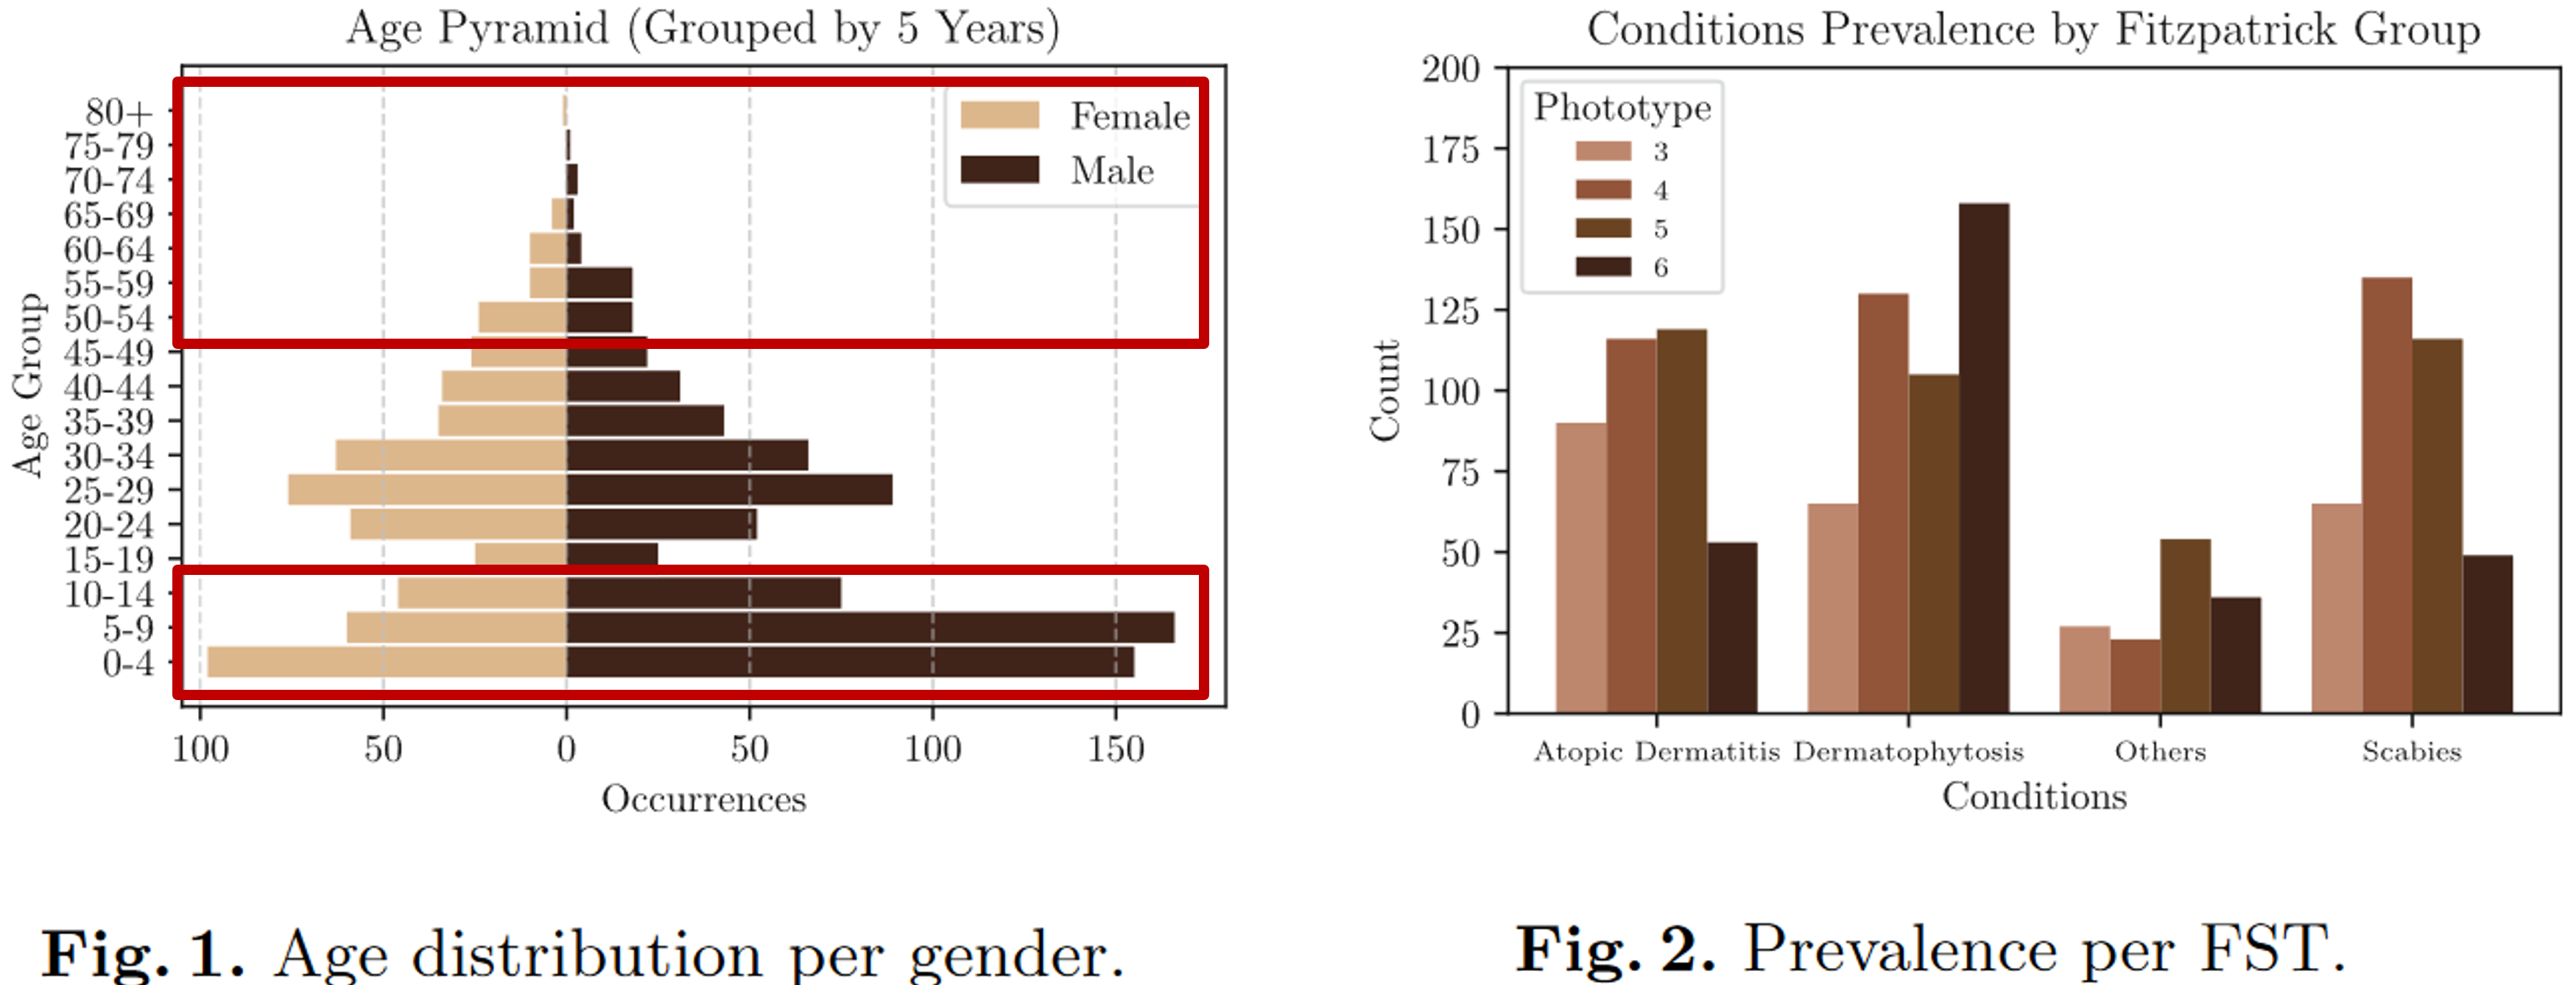
\includegraphics[width=0.9\textwidth]{figures/PASSIONDatasetDistributionPotentialImbalances.png}
			\caption{PASSION dataset distributions by \textcite{Gottfrois2024} - highlighting potential imbalances}
			\label{fig:PASSIONDistrImbalances}
		\end{figure}
		
		These findings highlight representation disparities across several demographic and clinical factors. Such disparities should be accounted for during training and fairness evaluation, especially when assessing subgroup-specific performance.
		
		It is important to note that the provided analysis only is a high-level overview at the group level. Detailed subgroup representation has not yet been assessed in details. Due to the time limits of this thesis, this was deferred in favor of executing the stratified split experiment.
		
		To enable subgroup-level representation analysis, group-level dataset representation script should be extended accordingly. As the script output will increase substantially, manual comparison may become impractical. Therefore, automating the comparison and generating summaries of the largest disparities is recommended.
		
		
		\section{Reproducing PASSION Results}
		The overall model performance was consistent with the results reported in the PASSION paper.
		
		However, the group-level performance results could not be reproduced. Multiple inference runs with the same model and dataset produced inconsistent results. Introducing metadata linkage via filenames resolved this issue and provided stable, reproducible results. This confirms a reliable association between predictions and metadata, which is critical for fairness analysis.
		
		Currently, the checkpoint handling supports only evaluation. Additional adjustments are needed to fully support resumed training, particularly to ensure correct and reproducible handling of epochs and cross-validation folds.
		
		
		While these extensive code improvements reduced the time available for fairness analysis, they are a critical enhancement to the robustness and usability of the PASSION evaluation.
		
		\section{PASSION Baseline Fairness Assessment} \label{sec:evaluation}
		
		The baseline fairness performance of \texttt{ResNet50} and \texttt{ResNet18} was assessed. This evaluation represents a reproducible baseline against which the impact of mitigation methods can be measured.
		
		\begin{itemize}
			\item \textbf{Baseline ResNet50:} \todo{[Insert Equalized Odds Difference/Ratio metrics here per subgroup and model level aggregation]}
			\item \textbf{Baseline ResNet18:} \todo{[Insert Equalized Odds Difference/Ratio metrics here per subgroup and model level aggregation]}
		\end{itemize}
		
		Although minor performance differences between the two model versions were found, the subgroup-level fairness trends proved largely consistent. Therefore, \texttt{ResNet18} was considered a valid substitution model for experimentation in this thesis.
		
		Further conclusions are summarized in the following subchapters.
		
		\subsection{Subgroup-Level Insights}
		Using the aggregation of class-level equalized odds metrics, the assessment revealed substantial variance across subgroups. Privileged and underprivileged subgroups are consistently identifiable.
		
		While some groups showed stable behavior across classes, others shifted category depending on the evaluated class, which underlines the importance of per-class fairness computation in multiclass settings.
		
		\subsection{Pipeline Challenges}
		
		Several technical limitations impacted the reliability and completeness of the fairness assessment:
		\begin{itemize}
			\item Fairlearn’s default multiclass handling is limited. To overcome this, a custom implementation was required, which introduces complexity and potential inconsistencies with the intended methodology of researchers.
			\item In the report part where subgroups are classified regarding privilege level, some subgroups were suppressed. This affects fairness analysis negatively. The comparison to the fairlearn output revealed this issue. This proves that it is preferable to use well-established, tested libraries for whenever possible.
			\item Manual aggregation of subgroup-level to model-level metrics is currently not automated, reducing reproducibility and increasing error risk.
		\end{itemize}
		
		Despite these challenges, the evaluation successfully surfaced subgroup disparities, supporting claims that fairness analysis on subgroups is important for reducing biases in dermatology models, including PASSION.
		
		\subsection{Aggregation Trade-offs}
		Aggregating fairness metrics at subgroup and model level provided helpful summaries but hide subgroup-specific effects. This must be considered when interpreting aggregated metrics.
		
		The proposed aggregation strategy was implemented due to the absence of ready-to-use multiclass equalized odds metrics in fairlearn or similar libraries. This illustrates the need for researchers to work together and implement suggested methodology improvements in the state of the art libraries.
		
		\subsection{Outlook on Evaluation Improvements}
		\todo{probably move to outlook}
		
		The current evaluation pipeline lays a solid groundwork but needs refinement:
		\begin{itemize}
			\item Replace confusion-matrix-based fairness calculations with direct \texttt{MetricFrame}-based computation to streamline and unify the process.
			\item Improve subgroup handling to include low-support groups more reliably, potentially via resampling or relaxed filtering.
			\item Automate the aggregation steps and document all assumptions clearly to enhance reproducibility.
		\end{itemize}
		
		In future work, incorporating multiple training seeds per setup will be essential for drawing statistically valid conclusions about fairness across model variations and mitigation methods.
		
		
	\chapter{Outlook}
		\baaCriteria{Reflexion der eigenen Arbeit, ungelöste Probleme, weitere Ideen.}
		\baaCriteria{Die Ergebnisse und Empfehlungen schaffen einen konkreten Mehrwert für die Auftraggebenden. Einschränkungen und Grenzen werden kritisch diskutiert und die nächsten Schritte im Ausblick festgehalten, so dass die Ergebnisse direkt in der Praxis weiterverwendet und/oder angewendet werden können.}
		
		This chapter summarizes the concrete recommendations to overcome the limitations of the current work. This includes e.g., revising the metadata used in PASSION, and extending the analytical tools used.
		
		It also provides ideas, such as adding more diverse data and combining PASSION with other dermatology datasets to improve bias detection and aim for a more complete dataset.
		
		These measures aim to enhance the practical applicability of the results and support the development of fair, generalizable \gls{ML} models in dermatology.
	
		
		\section{PASSION Dataset Improvements}
		To improve the fairness assessment capabilities of the PASSION dataset, the following dataset improvements are proposed:
		\begin{itemize}
			\item Include the missing metadata attributes identified in \autoref{chap:datasetAssessmentMetadataEvaluation} (e.g., socioeconomic status, clinic type, image quality) to enable a more comprehensive fairness evaluation. Ensure to assess the ethical implications before collecting such data.
			\begin{itemize}
				\item Investigate whether \textit{ethnicity} and \textit{disabilities} influence the presentation or prevalence of dermatological conditions before adding them to the dataset.
			\end{itemize}
						
			\item Clarify the intended purpose of the \textit{country} variable, and replace or supplement it with more precise alternatives, as discussed in \autoref{chap:datasetAssessmentMetadataEvaluation}.
			
			\item Refine the "other" condition category by breaking it down into more specific labels to improve diagnostic granularity and fairness assessment per condition.
			
			\item Incorporate healthy skin samples into the dataset to allow for a more balanced classification task and to mitigate potential bias.
			
			\item Explore whether combining PASSION with other dermatology datasets enhances generalization across the full \gls{FST} range. \todo{add point to consider to use other categorizations}
		\end{itemize}
		
		
		\section{Training Process Improvements}
		To enable full reproducibility and extensibility, further work should include:
		
		\begin{itemize}
			\item Finalizing checkpoint loading support for resumed training by correctly tracking and reloading epochs and folds.
			\item Incorporating automated tests to verify linkage integrity and model reproducibility.
		\end{itemize}
		
		
		\section{Fairness Assessment Process Improvements}
		The measures to improve the fairness assessment process further are:
		\begin{itemize}
			\item Extend the existing dataset representation script, as described in \autoref{chap:datasetAssessmentExecution}, to support subgroup-level analysis and automated comparison.
		\end{itemize}
		
		
		\section{Fairness Assessment Results Extension}
		\todo{@Proofreaders: habt ihr einen besseren Namen für dieses Kapitel? Es geht mir darum, dass weitere Analysen / Fairness assessments gemacht werden sollten}
		The existing fairness assessment results can be extended with those actions:
		\begin{itemize}
			\item Perform the representation analysis of relevant subgroups, as described in \autoref{chap:datasetAssessmentMethod} using the extended script, to determine whether observed unfairness stems from distribution imbalances at subgroup level.	
			
			\item Evaluate model performance across \gls{FST} types V and VI more closely and take measures if bias exist. \todo{check if this will still be needed}
		\end{itemize}
		
		
		Implementing these measures will enhance the dataset’s ability to support fair, robust, and generalizable \gls{ML} models in dermatology.
	
	
	\chapter{currently working on}
	
	\chapter{PASSION Baseline Fairness Assessment}
	
	
	
	
	
	\section{Outlook} \label{sec:outlook}
	
	
	In summary, the evaluation infrastructure and insights established in this thesis provide a meaningful first step toward robust fairness assessments in PASSION. With technical extensions and methodological refinements, it can evolve into a comprehensive toolset for bias detection and mitigation in dermatology and beyond.
	
	The fairness evaluation presented in this thesis revealed critical insights into subgroup disparities and pipeline limitations within the PASSION project setup. While the implemented approach provided a reproducible and structured baseline, several directions for future work have emerged to improve the robustness, generalisability, and reproducibility of fairness assessments.
	
	\subsection{Metric Implementation and Evaluation Consistency}
	
	As discussed, the current fairness evaluation relies in part on confusion-matrix-based metric computations. Replacing these with direct use of Fairlearn’s \texttt{MetricFrame} functionality across all fairness metrics would ensure a unified calculation standard and reduce implementation complexity. This would also increase consistency with other fairness research and future-proof the pipeline against methodological updates in fairness literature.
	
	\subsection{Improved Subgroup Handling}
	
	The suppression of low-support subgroups due to Fairlearn’s internal handling and manual filtering mechanisms may bias the evaluation. This highlights the need for a more sophisticated strategy to include or resample underrepresented subgroups without compromising statistical reliability. Future efforts should aim to ensure that all relevant subgroups are fairly assessed, particularly in the context of medical datasets where representation imbalances are common.
	
	\subsection{Automation and Documentation of Aggregation}
	
	Currently, the aggregation of fairness metrics from class to subgroup to model level involves manual steps. These introduce the risk of inconsistency and reduce reproducibility. Automating these aggregation procedures with fully transparent logic and clearly documented assumptions would significantly improve the interpretability and replicability of fairness assessments. Where applicable, sensitivity analyses of aggregation strategies should be added to evaluate their impact.
	
	\subsection{Statistical Robustness through Multiple Seeds}
	
	One key limitation of this work is the single-seed evaluation due to time and computational constraints. In fairness research, especially with deep learning models, results can be sensitive to random initialization and data splits. As recommended in \textcite{Valentim_2019}, future assessments should include multiple training and evaluation runs with different seeds to draw statistically significant conclusions about model fairness and mitigation impact. The current pipeline provides a foundation for such extensions.
	
	\subsection{Library and Methodology Development}
	
	The absence of well-established multiclass fairness implementations, particularly for metrics like equalized odds, required custom adaptations. This points to a broader need within the research community to extend existing libraries like Fairlearn to better support multiclass and subgroup-level analyses. Contributing the implemented methods and findings back to these open-source tools would benefit both the PASSION project and the wider fairness research community.
	
	\subsection{Broader Context and Integration}
	
	While this thesis focused on subgroup-level fairness analysis, future work could integrate fairness metrics into clinical utility assessments and decision-making contexts. This would enable a more holistic evaluation of trade-offs between fairness and clinical performance, which is essential for practical deployment in medical settings.
	

	
	
	

	\chapter{writing ongoing TODO REMOVE THIS CHAPTER}\todo{remove this chapter}
	\todo{put this somewhere in the outlook} Checkout this paper which suggest further methods and a flowchart to select the right fairness metric \textcite{Barr_2025}
	
	
	\todo{add to the stratified split experiment }: Cross-validation folds were removed to reduce evaluation time, it did not help that the gpuhub shut down your virtual machine after a while (2-3 days?), interrupting long (chained) experiment runs. Bc the checkpoint handling is not working yet for continuing training (only fixed that I can reload checkpoints for evaluating on the model again), this meant that some parts of the experiment had to be executed multiple times. Strongly suggest that the checkpoint handling is improved further by the passion team.
	
	
		\begin{itemize}
			\item \textbf{Tooling Support.}
			While the provided scripts enable basic demographic visualization, they lack functionality for intersectional subgroup analysis or fairness metric evaluation (e.g., \textit{equalized odds}).
		\end{itemize}
	
		\subsection{Bias Evaluation in PASSION}
		\todo{fix this writing}
		\paragraph{Methodology}
		In order to evaluate which biases are there in PASSION dataset, I need to
		\begin{itemize}
			\item reproduce the results of the paper using the PASSION evaluation project with the PASSION data to see a) verify the paper results, b) check what analysis data is available for the evaluation (the paper provides probably a summary), c) check what code can be reused and what needs to be adapted
			\item evaluate what data is missing to do evaluate the fairness and biases
			\item adapt code so that the relevant data is generated to be able to compute the relevant information
			\item GPUHub from HSLU is used, \todo{maybe add some machine information}
		\end{itemize}
		
		
		\rawcitationusedstart
		https://www.mdpi.com/2227-7102/14/2/136
		Equalized Odds (EO)	 𝑃(𝑌̂ =1|𝑌=𝑦,𝑆=1)−𝑃(𝑌̂ =1|𝑌=𝑦,𝑆=0),∀𝑦∈{0,1}
		We extend the fairness metrics, as described in Table 2, for non-binary sensitive attributes by considering a one-versus-rest approach for unfairness calculation. More specifically, to calculate the unfairness gaps, we consider each subgroup as 𝑆=1
		and compare it against the rest 𝑆=0
		(i.e., all other subgroups), one at a time. We mainly focus on racial disparities; however, our proposed approach for auditing fairness and investigating the imputation impact can be extended to use other sensitive attributes. For example, the decision-maker can use “gender” as a sensitive attribute.
		
		
		
		Missing data: Ignoring missing data is not an effective approach to handling missing values, and more importantly, it can result in predictive disparity for minority groups. While many education-related studies have addressed the challenges of missing data, as discussed, little is known about the impact of different imputation techniques on fairness outcomes in the final model. This project aims to address this gap by considering the three aforementioned imputation strategies.
		
		https://proceedings.mlr.press/v108/awasthi20a.html
		BiasY =y(Yb) =Pr h		Yb = 1	Y = y, A = 0i −Pr h	Yb = 1 		Y = y, A = 1i				.
		\rawcitationusedend
		
				
		
		
		\paragraph{Execution}
			In order to run the reproduction of the PASSION results on GPUHub, some minor changes in the loading process for the metadata had to be done. The required changes will be contributed to the code base to make the reproduction easier for others. \todo{do that then ;)}
			All 4 experiments where ran to get a broad overview of the results. The results of the 4 experiments contained the same scores as the ones mentioned in the paper. The scores are given separately for each demographic groups, either based on skin type or gender. There is no data for subgroups available. \todo{add results from age and center experiments}
			For the conditions classification, the provided scores per demographic group in the paper are the average scores over all classes. The variance/deviation of the averages in the scores based on the condition varies between the groups. E.g., the F1 score for \gls{FST} VI is 0.71$\pm$0.11 (total support 87) while for \gls{FST} it is 0.73$\pm$0.04 (total support 254). 
			The detailed information can be found in the attached logs
			% \todo{add logs from the file C:\\Users\\nadja\\OneDrive\\HSLU\_Nadja\\BAA\\baa\_on\_git\\results\\reproducing\_PASSION\_results}.
			
			The available data allows to compute the equalized odds fairness. \todo{describe which fairness methods to use why}
			In order to be able compute the subgroup fairness, the test results need to be split further into the subgroups. \todo{check exactly how to calculate subgroup fairness and whether there is already an algorithm for it, same for equalized odds}
			
					
			To reproduce all 4 experiments, the training ran took roughly \todo{add: it started on 24.4. roughly at 7 o clock, took until ca. 16.4., 13:00, the two other experiments started on 26.4. 17:30} hours since there where no model checkpoints available. This runtime is not feasible for each new training using a mitigation method, especially because the GPUHub seems to cancel the script after roughly 2 days, which means that each experiment needs to be started independently.
			Since this runtime it is not feasible to use for every mitigation run, the following adaptations where made \todo{add improvements described in protokol week 9}
			
			
			checkpoint handling was a bit broken
			runs x and x1 showed, that my code was reproducible while theirs was wrong
			--> running on passion model checkpoint without loading the rest of the infos in the checkpoint
			----> confirmed, that my calculations are reproducible while theirs are not; see commented out file names for comparison
			% experiment_standard_split_conditions_passion__bias_test_BIG_MODEL_reloaded_from_checkpoint.circ vs 		
			% experiment_standard_split_conditions_passion__bias_test_BIG_MODEL.circ
			also tested on another checkpoint, same behaviour, not cached results though
			
			
			no implementation of subgroup fairness found --> calc eq odds for subgroups
			
			
			The results in the PASSION results where reproducable only on the whole model level, but not for the groups. There was no subgroup analysis availbale.
			After adapting the data linkage in the PASSION evaluation code, the results where available when in the PASSION evaluation code. 
			
			
			The smaller model performance was used for the baseline. The Fairness results differ a bit from the bigger model, but it can still serve as a baseline.
			\todo{add somewhere that only the conditions classifier is used in this thesis, the impetig classifier should also be checked. (code is generalized, but must be tested)}
		\paragraph{Evaluation and Validation}
			A first analysis shows issues regarding xy in the big model and y in the small model.
			
			There are some differences in the metrics per class based on the model size. To investigate each class individually would require more effort which should be done later. The provided scripts can be used to generate the required data. \todo{add specific info in the attachement}
			Overall, the balanced accuracy for the small model = 0.69, big model = 0.7
			
							small	big
			Macro F1-Score: 0.69	0.71
			Precision: 		0.68	0.71
			Sensitivity:	0.69	0.71
			
			FST - 5 privileged in both
			6 underprivileged in both
			4,3 priviledged in big, avg or slightly underpriviledged in small
			
			Sex - no bias in small model, big model biased towards women; TPR ↑ (0.73), FPR ~ (0.09), m TPR ↓ (0.69), FPR ~ (0.10)
			
			Age - only slight differences between the models
			0-14; 25-29 priviledged
			20-24; 30-69 underpriviledged
			70+ not represented in test data	
			
			FP and sex - big model: FST 3 only men avg, f priviledged; FST 6 - men and women underprivileged
			small model: 3m priviledged, 3f underprivileged, 4 and 6 m underprivileged, f privileged
			
			
			
			here only the big model analyzed
			FP and age - more or less the same as age alone indipendent of skin type, besides skin type 6 which more often drags them down
			35-54 is more often well of with Skin type 3-5 though
			
			
			Age and Gender - f00-34 privileged! others avg / slightly higher FPR (small model privileged f00-34, m00-15;m25-29, m35-39)
			m 15-59 clearly underprivileged (same in small model)
			
			
			FP, age, gender, often only low support found, which puts more record in the unclear section.  
			
			
			country: Guniea much better on small model
			bacc 0.64, macro prec 0.63, sensivity: 0.65, F1 0.64
			big:
			bacc 0.58, macro prec 0.56, sensivity: 0.58, F1 0.56
						
			madagascar, bigger slightly better
			malawi bigger better
			tanzania exactly the same
			
			Tanzania in both majorly underprivileged
			Malawi majorly privileged
			
			FP and country: small model: Madagascar underprivileged in 4,6; 5 overprivileged;  
			Tanzania, only 4 and 5 FSTs, but both perform badly
			Malawi performs better as there are no records darker skin types
			Guinea and Skin Type 6 perform better than others
			
			big model: Madagascar FST 6 performs badly as well as tanzania; Guinea 6 is a bit worse than in the small model, but still quite good
						
			
			country and age: malawi is always privileged, tanzania under privileged
			madagascar and guinea more or less show the same results as gender alone
			
			
			compare from === Grouping: fitzpatrick, sex, country ===
			
			
			for certain subgroups, also malawi was underperforming.
			
			--> conclusion: sex, skin type and country hold the most clear biases. Since the aim of the dataset is to reduce bias on darker FSTs, especially the skin type issues are crucial - but they could also be linked to the country.
			Limitations: not all subgroup could be investigated in depht, especially the cross categories regarding age.
			
			
			% C:\Users\nadja\OneDrive\HSLU_Nadja\BAA\baa_on_git\results\reproducing_PASSION_results\small_model
			% C:\Users\nadja\OneDrive\HSLU_Nadja\BAA\baa_on_git\results\reproducing_PASSION_results\big_model
			
			
			
			
			
	\subsection{Stratified Split}
		\paragraph{Methodology}
		
		\rawcitationstart
		Furthermore, another version of each dataset was created with all features using a one-hot (or 1-of-K) encoding scheme [5] after being discretised, meaning that they are represented by binary dummy variables. We refer to this as the one-hot encoded version of a dataset.
		\autocite{Valentim_2019}
		The age attribute was discretised into two bins defined by a value greater than or equal to 25, a threshold that was set based on the findings reported by [26]. \autocite{Valentim_2019}
		
		Model Assessment
		We performed five-fold cross-validation with the help of the methods provided by Scikit-learn [8]. In addition to the standard version of cross-validation (normal-cv), the experiments were repeated with stratification (stratified-cv) so as to maintain the class distributions of the original data. Furthermore, each configuration was run with 30 different seeds for the random generators.
		
		We selected fairness metrics which can be applied to the datasets and to the predictions made by the models, so as to be able to compare the unfairness in the predictions to that originally found in the training data. The selected set of metrics includes statistical parity difference (CVS), disparate impact (DI), and the normalised prejudice index (NPI).
		
		The F1-score is more suitable when dealing with imbalanced datasets. However, we also include accuracy in our analysis to facilitate the comparison with previous work. \autocite{Valentim_2019}
		
		Fairness Comparison Between Data and Predictions
		Besides performing our analysis based on the fairness metrics mentioned in III-E, we computed the ratio between the CVS in the predictions and the CVS found in the data subset used to train the models (CVS Ratio), as well as a similar ratio regarding the NPI (NPI Ratio). These ratios give an indication of whether the unfairness in the training data was increased or reduced under each configuration. A value of 1 indicates that the unfairness in the predictions is the same as in the training data, an absolute value greater than 1 means that the unfairness in the predictions is greater, and an absolute value lower than 1 means that the model makes fairer predictions than the procedure which produced the true labels of the training data. A DI Ratio was not computed since it would be difficult to interpret the results. \autocite{Valentim}
		Comparison
		-->  How to compute the ratios between models:
		Let’s say you have two or more models: Model A, Model B, ..., Model N.
		
		And you compute the fairness metric (e.g., CVS) on each model’s predictions over the same dataset.
		
		Then, define a relative fairness ratio as follows:
		
		Model-vs-Baseline Fairness Ratio
		Choose one model as a baseline (e.g., the best, worst, or most standard one), and compare each other model to it:
		CSV / NPI = fairness metrics
		CVS RatioModel𝑋 = CVS (Model X) / CVS(Baseline Model)
​		NPI RatioModel𝑋 = NPI (Model 𝑋) / NPI(Baseline Model)
		
		Interpretation:
		Ratio = 1: Model X has the same fairness as the baseline.
		Ratio > 1: Model X is less fair (greater disparity or bias) than the baseline.
		Ratio < 1: Model X is fairer than the baseline.
		
		This approach is fully compatible with comparisons across models, even if you don’t consider the training data's fairness.
		
		\rawcitationend
		
		
		
		\paragraph{Execution}
		1. evaluating predifined dataset split regarding stratification
		
		
			
		since country, fitzpatrick and sex has been identified to have biased outcomes, they have to be checked most thoroughly 
		
		2. 
		
		\paragraph{Evaluation and Validation}
		1. from the data analysis, \todo{add to appendix} the data is pretty well distributed for most attributes. %C:\Users\nadja\OneDrive\HSLU_Nadja\BAA\baa_on_git\results\reproducing_PASSION_results\analyzing_dataset_split	
		Basically equal: Country, conditions\_PASSION
		Almost equal: most ageGroup and impedig are 
		Bigger differences: fitzpatrick, sex, some ageGroups
		sex: contradictory to the bias towards female, the dataset is skewed to male, with even more males which was trained on. Therefore, this data skew might not be the source of the bias in the model.. 
		
		train: f: 539 (40.74\%) m: 784 (59.26\%)
		test: f: 152 (46.06\%) m: 178 (53.94\%)
		overall: f: 691 (41.8\%) m: 962 (58.2\%)
		
		
		FST types 4 and 5 are overrepresented in training, which could cause the biases on the big model.
		
		
		What I should do:
		1 random split, 1 stratified on condition and country (what probably was the split from passion), 1 stratified with FST condition country, 1 stratified with FST condition country sex 
		
		
		1. change dataset, so that those splits are reflected in validation data
		2. train models with no folds on the train and validation (simply use other split file in the begining)
		3. while training is running investigate how fold splits the data
		
		
		
	
		for the country, the distribution is already almost the same for all splits, with Tanzania clearly underrepresented. On this variable, stratified splitting should be kept for sure. More data should be captured from Tanzania - it could be differences with the data quality which lead to different results.
		
			
			

		% Lists and References
		\newpage




	\todo{probably remove this}
	%\chapter{\glossaryname \todo{probably remove this}}
		%\printglossary[title={}]
	%\todo{Add to ToC of content somehow and fix chapter numbers}
	%\listoffigures
	%\listoftables
	\todo{Add List of Formulas if necessary}
	\todo{add \gls{AI} declarations somewhere}
	
	
	\chapter{\bibname}
		\printbibliography[heading=none]
		
		%\bibliographystyle{ieeetr}
		%\footnotesize\bibliography{references}
		
		
		%----------------------------------------------------------------------------------------
		%	APPENDIX
		%----------------------------------------------------------------------------------------
		\newpage
		\appendix
		\begin{appendices}
			\baaCriteria{Projektspezifisch können weitere Dokumentationsteile angefügt werden wie: Aufgabenstellung, Projektmanagement-Plan/Bericht, Testplan/Testbericht, Bedienungsanleitungen, Details zu Umfragen, detaillierte Anforderungslisten, Referenzen auf projektspezifische Daten in externen Entwicklungs- und Datenverwaltungstools etc.}
			
			\todo{fix appendices chapters, wtf}
			\todo{also move the bibliography potentially after the appendices, idk}
			%\renewcommand{\thechapter}{Appendix \Alph{chapter}}
		
	
			\chapter{PASSION Data Analysis Scripts}\label{app:PASSIONdataAnalysisScripts}
			The PASSION team provides a \gls{JupyterNotebook} with code examples and analysis scripts. They are listed in \autoref{tab:PASSION_scripts} together with their relevance to this thesis. The most relevant scripts are those related to demographic distributions of the chosen attributes, since they help identifying potential data imbalances. Scripts that lay the foundation for further analysis are somewhat relevant, while all other scripts are irrelevant for this thesis.
			
			\begin{table}[H]
				\centering
				\begin{threeparttable}
					\begin{tabularx}{\textwidth}{>{\hsize=.25\hsize\raggedright}X>{\hsize=.41\hsize}X>{\hsize=.34\hsize}X}
						\toprule
						\textbf{Script Title}       & \textbf{Description} & \textbf{Relevance - Reasoning}       \\ \midrule
						Distribution of \glspl{FST} &
						Counts and visualizes the skin type distribution  &
						\textbf{High} - Insight into demographic distributions \\
						\hline
						Regrouping Malawi and Tanzania to EAS &
						Data aggregation due to dataset size and geographical proximity &
						\textbf{Medium} - Might impact interpretation of the results of the following scripts \\
						\hline
						Linking CSV Data with Image Files & 
						Mapping between data records and images. &
						\textbf{Medium} - Basis for other analyses \\
						\hline
						Extracting and Comparing Subject IDs &
						Dataset verification regarding completeness &
						\textbf{Low} - No insight in regards of demographic distribution \\
						\hline
						Conditions by Country &
						Correlation between clinical conditions and country &
						\textbf{Low} - The attribute \textit{country} is out of scope of this thesis \\
						\hline
						Body Localizations by Conditions &
						Correlation between the condition and primarily affected body parts &
						\textbf{Low} - No insight in regards of demographic distribution \\
						\hline
						Impetigo Cases &
						Total count of impetigo cases and proportion to all cases &
						\textbf{Low} - No insight in regards of demographic distribution\tnote{*} \\
						\bottomrule
					\end{tabularx}
					\begin{tablenotes}
						\footnotesize
						\item[*] Research is divided on which demographic factors influence the prevalence of impetigo \autocites{Romani_2017}{Aleid_2024}.
					\end{tablenotes}
				\end{threeparttable}
				
				\caption{PASSION dataset - existing analysis scripts \autocite{Gottfrois2024}}
				\label{tab:PASSION_scripts}
			\end{table}
			
			%%\iftrue
%\iffalse
%
%\documentclass[12pt, a4paper, oneside]{book}
%% todo: fix appearances
%\usepackage[backend=biber]{biblatex}
%\addbibresource{references.bib}
%
%\usepackage{comment}                            % having comment sections \begin{comment} \end{comment}
%\usepackage[utf8]{inputenc}						% charactere interpretation
%\usepackage{amsmath}							% math package
%\usepackage{amsfonts}							% font package for math symbols
%\usepackage{amssymb}							% symbols package - definition of math symbols
%\usepackage{listings}							% package for code representation
%\usepackage{csquotes}       % Quotation support
%\usepackage{graphicx}							% for inclusion of image
%\setlength {\marginparwidth }{2cm}
%\usepackage{todonotes}
%\usepackage{booktabs}       % Better tables
%\usepackage{caption}        % Better captions
%\usepackage{subfig}								% to arrange figures next to each other
%\usepackage{float}								% text style surrounding images
%\usepackage{threeparttable}
%\usepackage{tikz}								% used to place logos on title page
%% \usepackage{gensymb}							% for special characters such as °
%\usepackage{titlesec}
%\usepackage{multirow}
%\usepackage{siunitx}
%\usepackage{tabularx}
%\usepackage{tikzscale}
%% Format chapter titles without "Chapter X" prefix
%\titleformat{\chapter}[hang]
%{\normalfont\LARGE\bfseries}  % Style: Large bold text
%{\thechapter}                 % Number format: Just the number
%{1em}                         % Space between number and title
%{}                            % Code before the title (empty)
%\usepackage{hyperref}
%\hypersetup{hidelinks}
%\usepackage[acronym]{glossaries}         				% package for glossary
%\makenoidxglossaries
%\newacronym{HSLU}{HSLU}{Lucerne University of Applied Sciences and Arts}
\newacronym[see={[Glossary:]{fitzpatrick-skin-type}}]{FST}{FST}{Fitzpatrick skin type\glsadd{fitzpatrick-skin-type}}
\newacronym{ML}{ML}{Machine Learning}
\newacronym{AI}{AI}{Artificial Intelligence}
\newacronym{FPR}{FPR}{false positive rate}
\newacronym{TPR}{TPR}{true positive rate}
                                % include acronyms.txt file
%\newglossaryentry{fitzpatrick-skin-type}{
	name={Fitzpatrick skin type},
	plural={Fitzpatrick skin types},
	description={A skin classifier based on the skins' reaction to ultraviolet light, developed by dermatologist Dr. Thomas Fitzpatrick \autocite{Gottfrois2024}}
}
\newglossaryentry{JupyterNotebook}{
	name={Jupyter Notebook},
	description={Executable files, often used in ML to write Python code and add explanations in text form}
}
\newglossaryentry{gpuhub}{
	name={GPUhub},
	description={\gls{HSLU}’s server infrastructure for GPU-related computing. It provides isolated environments with JupyterLab access for developing and running \gls{ML} workflows}
}
\newglossaryentry{pediatric}{
	name={pediatric},
	description={A medical term for infants, children and adolescents \autocite{Farlex_nodate}}
}
\newglossaryentry{proxyVar}{
	name={proxy variable},
	plural={proxy variables},
	description={"one or more variables that encode the protected attribute with a substantial degree of accuracy" \autocite{Wang_2021}}
}
\newglossaryentry{teledermatology}{
	name={teledermatology},
	description={dermatological care from a distance, supported by modern technology \autocite{Pala_2020}}
}
\newglossaryentry{Fairlearn}{
	name=Fairlearn,
	description={A Python library for assessing and improving fairness in machine learning models. It supports various fairness metrics and mitigation techniques, especially for binary classification tasks \autocite{Fairlearn_nodate}}
}
\newglossaryentry{Equalized-Odds-Difference}{
	name={equalized odds difference},
	description={The absolute difference in true positive and false positive rates between subgroups, used as a group fairness metric \autocite{Fairlearn_nodate}}
}
\newglossaryentry{Equalized-Odds-Ratio}{
	name={equalized odds ratio},
	description={The ratio of true positive and false positive rates between subgroups, used as a group fairness metric \autocite{Fairlearn_nodate}}
}                                % include glossary.txt file
%\graphicspath{{figures/}}						    % set path of graphics folder
%% mentioned in header
%\newcommand{\tblWidthDescription}{\hsize=0.6\hsize\raggedright}
%\newcommand{\tblWidthContext}{\hsize=0.2\hsize}
%%improved basic functionality
%\newcommand{\bolditalic}[1]{\textbf{\textit{{#1}}}}
%%indicate citations
%% Define a flag to track whether we're inside a raw citation block
%\newif\ifrawcitationactive
%\rawcitationactivefalse % Default: Not inside a raw citation block
%% Define color commands with conditional checking
%\newcommand{\rawcitationstart}{
%	\color{purple}\rawcitationactivetrue
%}
%\newcommand{\rawcitationend}{
%	\color{black}\rawcitationactivefalse
%}
%\newcommand{\rawcitationusedstart}{\color{violet}}
%\newcommand{\rawcitationusedend}{%
%	\ifrawcitationactive
%	\color{purple}  % If inside rawcitation, reset to purple
%	\else
%	\color{black}  % Otherwise, reset to black
%	\fi
%}
%\begin{document}
%\fi
	
	\begin{refsection}
		\chapter{List of Biases}\label{app:listOfBiases}
		The biases are categorized and the relevance for PASSION is added to their chapter title in italic, e.g. \textit{high}.
		
		\section{\textbf{Category:} Sampling Bias}
		Sampling biases occur when the process of collecting data results in samples that are not representative of the broader population. These biases affect the generalisability of machine learning models, especially in medical applications, where population diversity is crucial. According to \textcite{Mehrabi_2021}, non-random or selective sampling can lead to serious consequences in terms of fairness and effectiveness of AI systems.
		
		\subsection{Sampling Bias, \textit{high}}
		\begin{itemize}
			\item \textbf{Definition:} Bias introduced through non-random sampling of subgroups, leading to poor generalisation.
			\item \textbf{Example:} An ML model trained predominantly on patients from urban hospitals may underperform for rural patients.
			\item \textbf{PASSION Relevance:} PASSION aims to address dermatologic sampling bias against highly pigmented skin, but if the included data is not truly representative across populations (e.g., over-representation of certain regions), this could still result in sampling bias \autocite{Mehrabi_2021}.
			\item \textbf{Mitigation Strategy:} Ensure a truly random and inclusive sampling strategy across geography, socioeconomic status, and skin types.
		\end{itemize}
		
		\subsection{Selection Bias, \textit{high}}
		\begin{itemize}
			\item \textbf{Definition:} Bias arising when only a specific subset of the population is used, which is not representative.
			\item \textbf{Example:} Training a model only on adult data, when the target population includes children.
			\item \textbf{PASSION Relevance:} PASSION may suffer from selection bias if only data from severe dermatology cases in hospitals is used \autocites{Mester_2022}{Chakraborty_2024}.
			\item \textbf{Mitigation Strategy:} Include a broad variety of case severities and healthcare settings in the dataset.
		\end{itemize}
		
		\subsection{Systematic Selection Bias, \textit{high}}
		\begin{itemize}
			\item \textbf{Definition:} A form of selection bias where chosen samples differ systematically from the general population.
			\item \textbf{Example:} Including only hospitalized patients in a dataset, while most cases are treated in outpatient settings.
			\item \textbf{PASSION Relevance:} If PASSION uses data only from dermatology centers treating severe cases, it introduces systematic selection bias \autocite{Chakraborty_2024, c5,c6,c33}.
			\item \textbf{Mitigation Strategy:} Include mild, moderate, and severe cases from various clinical settings.
		\end{itemize}
		
		\subsection{Ascertainment Bias, \textit{high}}
		\begin{itemize}
			\item \textbf{Definition:} A systematic distortion arising from the method by which participants or data are selected for inclusion.
			\item \textbf{Example:} Studies on STD prevalence conducted only in public clinics may overlook patients from higher-income backgrounds who go to private practitioners.
			\item \textbf{PASSION Relevance:} If PASSION’s dataset is composed mostly of patients from certain types of clinics, it may not generalise well to other socioeconomic groups \autocite{Chakraborty_2024, c5}.
			\item \textbf{Mitigation Strategy:} Ensure that data is collected from a diverse range of sources, including both public and private healthcare facilities.
		\end{itemize}
		
		\subsection{Availability Bias, \textit{high}}
		\begin{itemize}
			\item \textbf{Definition:} Overreliance on easily accessible data rather than the most representative data.
			\item \textbf{Example:} Using only online available datasets for skin conditions may underrepresent rare diseases.
			\item \textbf{PASSION Relevance:} PASSION inherits availability bias by relying on FST scale–labelled datasets, which may not fully reflect global skin tone diversity \autocites{Chakraborty_2024, c9, c10}.
			\item \textbf{Mitigation Strategy:} Actively seek underrepresented data sources, especially for less common or less documented skin types.
		\end{itemize}
		
		\subsection{Survivorship Bias, \textit{medium}}
		\begin{itemize}
			\item \textbf{Definition:} Only using data from "survivors", i.e., subjects that make it through a certain threshold or are retained in the dataset, ignoring those who were lost earlier.
			\item \textbf{Example:} Evaluating the success of a treatment based only on patients who completed it, ignoring those who dropped out due to side effects.
			\item \textbf{PASSION Relevance:} If certain dermatology diseases are lethal or if the dataset excludes patients unable to attend the centers involved in PASSION, survivorship bias may be present \autocite{Mester_2022}.
			\item \textbf{Mitigation Strategy:} Account for dropout rates and include cases from a wide range of medical access points.
		\end{itemize}
		
		
		\section{\textbf{Category:} Representation Biases}
		Representation biases occur when a sample used to train or evaluate a machine learning model fails to adequately reflect the diversity of the target population. These biases can lead to underperformance for certain subgroups and may negatively impact the fairness and accuracy of a model in real-world applications. In the context of dermatology, these biases could result in skin diseases being underrepresented or misclassified in specific demographic groups, leading to poorer diagnostic outcomes for those populations.
		
		\subsection{Representation Bias, \textit{high}}
		\begin{itemize}
			\item \textbf{Definition:} Representation bias arises when the sample used to train a model does not adequately represent all subgroups of the target population, leading to missing or misrepresented characteristics in the data.
			\item \textbf{Example:} If a skin disease detection model is trained predominantly on skin types I-IV, it may struggle to accurately diagnose conditions in individuals with darker skin tones (FST skin types V-VI).
			\item \textbf{PASSION Relevance:} PASSION attempts to mitigate representation bias by including more FST skin types, but challenges may still exist. The dataset could still lack full representation of all diverse skin conditions and demographic factors, leading to potential misdiagnoses or underperformance for specific subgroups.
			\item \textbf{Mitigation Strategy:} A potential mitigation strategy could involve ensuring a more balanced representation of FST skin types, including rare and diverse skin conditions, and periodically reassessing the dataset to ensure comprehensive inclusion of all skin types across various demographics.
		\end{itemize}
		
		\subsection{Population Bias, \textit{medium}}
		\begin{itemize}
			\item \textbf{Definition:} Population bias occurs when the sample's demographic characteristics (such as age, gender, or ethnicity) do not align with the target population, leading to non-representative data.
			\item \textbf{Example:} If a dataset is predominantly comprised of one ethnic group, a model trained on this data may not generalize well to other ethnic groups, especially if the manifestation of skin diseases varies across ethnicities.
			\item \textbf{PASSION Relevance:} PASSION might be impacted by population bias if it is insufficiently diverse in terms of patient demographics (e.g., ethnicity, age). The dataset needs to ensure that skin diseases are accurately represented across different population groups to avoid skewing results and compromising diagnostic accuracy.
			\item \textbf{Mitigation Strategy:} A mitigation strategy could involve collecting data from diverse populations and ensuring the dataset reflects the target population’s demographic diversity, particularly for ethnicities and age groups that may exhibit different disease manifestations.
		\end{itemize}
		
		\subsection{Aggregation Bias, \textit{high}}
		\begin{itemize}
			\item \textbf{Definition:} Aggregation bias occurs when conclusions drawn from the entire population do not apply to individual subgroups, leading to incorrect or generalized assumptions. This bias arises when significant differences between subgroups (such as gender or ethnicity) are not properly accounted for.
			\item \textbf{Example:} A diagnostic model trained on a heterogeneous dataset might fail to capture how skin diseases manifest differently across genders or ethnic groups, potentially leading to misdiagnosis or unequal treatment recommendations.
			\item \textbf{PASSION Relevance:} Aggregation bias is a significant concern in PASSION, particularly since skin diseases can manifest differently across ethnicities, genders, or genetic backgrounds. The model needs to account for these variations to avoid generalized conclusions that might harm certain subgroups.
			\item \textbf{Mitigation Strategy:} To mitigate aggregation bias, the model should incorporate subgroup-specific data and analysis, ensuring that disease manifestations are correctly accounted for and tailored to different demographic characteristics.
		\end{itemize}
		
		\subsection{Simpson's Paradox, \textit{medium}}
		\begin{itemize}
			\item \textbf{Definition:} Simpson's Paradox is a form of aggregation bias where trends that appear in aggregated data may reverse when the data is disaggregated into subgroups. This paradox can lead to misleading conclusions if not properly addressed.
			\item \textbf{Example:} A dataset may show that skin disease detection is more accurate overall for a specific demographic group, but when the data is broken down by age or skin type, the trend reverses for certain subgroups.
			\item \textbf{PASSION Relevance:} Simpson’s Paradox could be an issue in PASSION if aggregated data from different subgroups results in misleading conclusions. For example, overall accuracy may appear high, but specific skin conditions in certain ethnicities or age groups could have lower accuracy when analyzed separately.
			\item \textbf{Mitigation Strategy:} A mitigation strategy would involve analyzing data at both the aggregated and disaggregated levels, ensuring that subgroup-specific trends are considered to avoid false conclusions or the reversal of apparent associations.
		\end{itemize}
		
		
		
		
		
		\section{\textbf{Category:} Measurement Biases}
		Measurement biases occur when the process of choosing, using, or measuring features leads to inaccurate or misleading results. These biases can emerge from various sources such as mismeasured variables, subconscious expectations of researchers, or inconsistencies in human annotation, and they can significantly affect the reliability of the dataset.
		
		\subsection{Measurement Bias, \textit{high}}
		\begin{itemize}
			\item \textbf{Definition:} Measurement bias occurs when features or variables are inaccurately measured or selected, leading to incorrect interpretations of the outcome.
			\item \textbf{Example:} If a proxy variable, such as country of origin, is used to infer ethnicity or genetic background, it could lead to misinterpretation of the data. For instance, the country of origin may not directly correlate with ethnic background, potentially skewing results in genetic or disease research \autocite{Mehrabi_2021}.
			\item \textbf{PASSION Relevance:} In the context of the PASSION dataset, measurement bias could arise if country of origin is misused as a proxy for ethnicity, which is not directly related to genetic predispositions or skin conditions. This could result in misleading conclusions about skin diseases across different demographic groups, potentially amplifying health disparities.
			\item \textbf{Mitigation Strategy:} To mitigate measurement bias in PASSION, careful consideration should be given to the choice of features used in the dataset. Avoiding proxy variables such as country of origin to infer ethnicity and instead focusing on genetically relevant factors could improve the accuracy of the data and its interpretation.
		\end{itemize}
		
		\subsection{Observer Bias, \textit{medium}}
		\begin{itemize}
			\item \textbf{Definition:} Observer bias occurs when researchers or testers influence the results by projecting their expectations or perceptions onto the data collection process, or when different observers report the same observation differently.
			\item \textbf{Example:} A researcher may subconsciously interpret certain skin disease symptoms differently based on their own expectations or biases, leading to inconsistent data collection or interpretation \autocite{Mester_2022}.
			\item \textbf{PASSION Relevance:} In PASSION, observer bias could affect the consistency and reliability of skin disease annotations. For example, a researcher might influence how they categorize or diagnose certain skin diseases based on their personal biases or experience. This could lead to inaccurate classifications, particularly for diseases that are subjective in appearance.
			\item \textbf{Mitigation Strategy:} To address observer bias in PASSION, standardized training for annotators and a clear, objective set of criteria for diagnosis should be implemented. Additionally, using multiple annotators and cross-checking results can help reduce the impact of individual biases.
		\end{itemize}
		
		\subsection{Annotator Bias, \textit{high}}
		\begin{itemize}
			\item \textbf{Definition:} Annotator bias is a form of observer bias where human annotators are influenced by personal background, expectations, or external factors, which can lead to inconsistent or skewed labeling of data \autocite{Montoya_2025}.
			\item \textbf{Example:} If an annotator is more likely to label a darker skin tone as "severe" or "critical" due to personal or cultural biases, this can introduce inaccuracies in the dataset, which may not be representative of the actual severity of the condition.
			\item \textbf{PASSION Relevance:} In PASSION, annotator bias could particularly affect the labeling of skin tones, which are highly subjective and dependent on individual perception. This bias could lead to inconsistent classifications of skin conditions across different demographic groups, which is critical when assessing dermatological diseases in a diverse population.
			\item \textbf{Mitigation Strategy:} To reduce annotator bias in PASSION, a diverse team of annotators should be trained to recognize and overcome their personal biases. Additionally, the annotation process should be regularly audited to ensure consistency, and the use of automated tools for initial labeling could provide more objectivity in the process.
		\end{itemize}
		
		\subsection{Recall Bias, \textit{medium}}
		\begin{itemize}
			\item \textbf{Definition:} Recall bias occurs when individuals do not accurately remember or report information due to selective memory, which can lead to misinterpretations or inaccurate conclusions in data analysis \autocites{Mester_2022}{Chakraborty_2024}.
			\item \textbf{Example:} If patients are asked to recall past skin conditions or treatments, they may forget important details, leading to inaccurate reporting in the dataset. This could affect the analysis of how different skin diseases develop or respond to treatments.
			\item \textbf{PASSION Relevance:} Recall bias may not be directly relevant in the context of PASSION since the dataset appears to rely on clinical observations and annotations rather than patient-reported data. However, if there is any patient input, such as in follow-up surveys or self-reported symptoms, recall bias could still influence the dataset.
			\item \textbf{Mitigation Strategy:} To mitigate recall bias, it would be important to gather more objective data through clinical observations or imaging, and ensure that patient self-reports are validated through corroborating medical records or consistent follow-ups.
		\end{itemize}
		
		\subparagraph{Potential Biases in PASSION}
		Measurement Bias: Country of origin should not be used as a proxy for ethnicity in the PASSION dataset, as it may not be directly related to genetic or disease factors. Additionally, annotator bias regarding skin tone labeling has been investigated in recent studies and should be addressed in PASSION's annotation process \autocite{Montoya_2025}.
		
		
		\section{\textbf{Category:} Research Biases}
		Research biases refer to the ways in which researchers' decisions, intentions, and contexts influence the outcomes of their studies, potentially introducing systematic errors that may affect the validity or generalizability of the findings.
		
		\subsection{Funding / Sponsorship bias, \textit{medium}}
		\begin{itemize}
			\item \textbf{Definition:} Funding or sponsorship bias occurs when research findings are consciously or unconsciously influenced by the expectations or interests of the study’s financial backers. This can lead to findings that favor the sponsor’s interests.
			\item \textbf{Example:} A dermatology study funded by a pharmaceutical company that produces skin disease treatment medications may emphasize the effectiveness of the company's products, even if there is no strong evidence supporting their superiority.
			\item \textbf{PASSION Relevance:} Funding bias could affect the PASSION dataset if the research or data collection process were influenced by sponsors or stakeholders with vested interests in certain outcomes. While this bias is not explicitly mentioned in PASSION, it is important for future studies to ensure that funding sources do not shape data interpretation or collection in a way that would lead to skewed or misleading results.
			\item \textbf{Mitigation Strategy:} To mitigate this, independent funding sources or transparent funding disclosure practices should be implemented. Additionally, external audits or independent validation of the findings can help prevent undue influence from sponsors.
		\end{itemize}
		
		\subsection{Data dredging bias, \textit{low}}
		\begin{itemize}
			\item \textbf{Definition:} Data dredging bias arises when researchers deliberately select statistical methods or models that lead to specific p-values or results, potentially making their hypothesis appear more likely to be true than it actually is.
			\item \textbf{Example:} A researcher testing multiple variables in a dataset might select those combinations that yield the most statistically significant results, even if the relationships between the variables were not hypothesized initially.
			\item \textbf{PASSION Relevance:} Given that PASSION is a large dermatology dataset, it could be vulnerable to data dredging if analysts test many variables or relationships without pre-specified hypotheses. This could lead to spurious findings or models that do not generalize well to new data.
			\item \textbf{Mitigation Strategy:} To avoid data dredging, a clear and well-defined hypothesis should be established before conducting any statistical tests. Additionally, cross-validation techniques and reporting of all tested models can ensure transparency in the research process.
		\end{itemize}
		
		\subsection{Hypothetical bias, \textit{not applicable}}
		\begin{itemize}
			\item \textbf{Definition:} Hypothetical bias occurs when responses to hypothetical questions do not reflect real-world behavior or preferences.
			\item \textbf{Example:} Asking participants how likely they would be to adopt a particular skincare treatment, without actually testing their behavior in real-world settings.
			\item \textbf{PASSION Relevance:} This bias is not applicable to the PASSION dataset, as the dataset does not involve hypothetical scenarios or self-reported intentions. The dataset primarily contains real-world medical data related to dermatology, which does not rely on participant speculation or hypothetical responses.
			\item \textbf{Mitigation Strategy:} Since this bias is not relevant to PASSION, no specific mitigation strategy is necessary.
		\end{itemize}
		
		\paragraph{Potential Biases in PASSION}
		Since the PASSION dataset is already published, the research biases might already be introduced. It is not feasible during the duration of this thesis to make an evaluation on those biases. Instead, I would recommend the PASSION team and researchers in general to check the list above carefully and take measures against them. Maybe, an external evaluation could help to detect and prevent those biases even better.
		
		
		\section{\textbf{Category:} Feature Representation Biases}
		Feature representation biases occur when the features or variables used in a model do not adequately capture the complexity of the problem or reflect all relevant aspects of the data, potentially leading to biased or incomplete predictions.
		
		\subsection{Omitted Variable Bias, \textit{high}}
		\begin{itemize}
			\item \textbf{Definition:} Omitted variable bias arises when key variables are left out of a model, causing the model to be unprepared to account for certain aspects of the data and potentially leading to biased or inaccurate predictions.
			\item \textbf{Example:} If a dermatology model only includes skin condition data but omits important demographic information such as ethnicity or age, it may fail to identify or misinterpret certain patterns in the data.
			\item \textbf{PASSION Relevance:} The PASSION dataset has an omission of ethnicity as a feature, which could lead to biased results. Certain skin diseases and their manifestation can vary significantly across different ethnic groups. Without this variable, the model may fail to capture important differences in the data, leading to inaccurate predictions or generalizations.
			\item \textbf{Mitigation Strategy:} To address this bias, it is important to include a comprehensive set of features, such as ethnicity, age, gender, and other demographic factors, which could help the model better account for variations in skin conditions across different populations.
		\end{itemize}
		
		\subsection{Collider Bias, \textit{medium}}
		\begin{itemize}
			\item \textbf{Definition:} Collider bias occurs when two variables influence a common third variable (the collider variable), and the analysis restricts sampling based on this collider, leading to a distorted or biased relationship between the variables.
			\item \textbf{Example:} In the case of skin disease models, if researchers only include patients who seek treatment for a specific skin condition (the collider), this may limit the analysis to a non-representative sample, potentially distorting the relationship between disease characteristics and other factors.
			\item \textbf{PASSION Relevance:} Although no specific collider bias has been identified in PASSION, it is important to consider that factors like patient willingness to seek treatment or the specific type of skin disease could act as collider variables. Restricting the dataset based on these factors might create a biased representation of the population.
			\item \textbf{Mitigation Strategy:} To reduce collider bias, it is important to ensure that the sample is as representative as possible of the broader population. Researchers should avoid restrictions that could inadvertently create a non-representative dataset and be mindful of how their sampling methods may introduce bias.
		\end{itemize}
		
		\subparagraph{Potential Biases in PASSION}
		The PASSION dataset may suffer from omitted variable bias, particularly with the lack of ethnicity data, which can affect the fairness and accuracy of dermatology models. Collider bias could also emerge depending on how the dataset is sampled or restricted based on treatment-seeking behavior or disease severity. It is important for researchers to monitor for these biases and take steps to mitigate them by ensuring that data collection and sampling strategies are inclusive and comprehensive.
		
		
		
		\section{\textbf{Category:} Imaging Biases}
		Imaging biases refer to the influence that technical variations, environmental factors, and other visual elements have on image-based classification systems. These biases can arise from issues such as the quality of the image, artifacts present in the image, or the field of view captured, which can all influence the performance of machine learning models.
		
		\subsection{Image Quality Bias, \textit{high}}
		\begin{itemize}
			\item \textbf{Definition:} Image quality bias occurs when the quality of an image—such as the zoom level, focus, or lighting—affects how a machine learning model classifies or diagnoses the image. Poor image quality can lead to misclassification or lower prediction accuracy.
			\item \textbf{Example:} If a dermatologist captures an image with insufficient lighting or poor focus, the model may struggle to identify skin conditions like melanomas, potentially leading to a misdiagnosis.
			\item \textbf{PASSION Relevance:} In the PASSION dataset, variations in image quality could lead to biased predictions. For instance, images captured under different lighting conditions or at varying zoom levels might cause the model to overfit to certain image qualities, mistaking them for certain conditions. This could reduce the model’s generalizability to diverse real-world conditions.
			\item \textbf{Mitigation Strategy:} To mitigate image quality bias, it is essential to standardize image acquisition protocols and pre-process images to normalize variations in quality. Implementing techniques like image enhancement and quality control during data collection could help improve model performance.
		\end{itemize}
		
		\subsection{Visual Artifact Bias, \textit{high}}
		\begin{itemize}
			\item \textbf{Definition:} Visual artifact bias arises from artifacts in dermatology images, such as hair, surgical ink markings, or other extraneous elements that could interfere with accurate classification of skin diseases.
			\item \textbf{Example:} A photograph of a skin lesion may contain hair or tattoos from previous medical procedures, making it more difficult for the model to identify the skin condition correctly.
			\item \textbf{PASSION Relevance:} The PASSION dataset may include dermatology images with artifacts like surgical markings or hair, which could confuse the model into associating these artifacts with the presence of a skin disease. This could lead to incorrect predictions, especially if the model cannot differentiate between the artifact and the actual lesion.
			\item \textbf{Mitigation Strategy:} To reduce visual artifact bias, it is important to implement preprocessing steps that remove or mask artifacts in images. This could involve techniques such as hair removal or the use of clean, artifact-free image samples for training.
		\end{itemize}
		
		\subsection{Field of View Bias, \textit{high}}
		\begin{itemize}
			\item \textbf{Definition:} Field of view bias occurs when the portion of the body or skin that is captured in an image is limited, affecting how well a model can classify a skin condition. Different angles, distances, or body parts in the view may lead to different prediction results.
			\item \textbf{Example:} If only a small portion of a skin lesion is captured in the image (e.g., just the edge of a mole), the model may miss critical features needed to correctly identify melanoma or other conditions.
			\item \textbf{PASSION Relevance:} In the PASSION dataset, field of view bias could emerge if certain lesions are captured from angles or in parts of the body that limit the information available for accurate classification. This could result in the model underperforming on images that are not representative of common views of skin conditions.
			\item \textbf{Mitigation Strategy:} To address field of view bias, the dataset should ensure that images are captured from standardized and consistent angles or distances. Augmenting the dataset with a variety of views from multiple angles could help improve the model's ability to generalize to unseen cases.
		\end{itemize}
		
		\subparagraph{Potential Biases in PASSION}
		The PASSION model could learn to associate unrelated visual effects, hair, body parts, or image quality with a disease, which could impact its performance. Ensuring standardized image acquisition methods and removing artifacts could mitigate some of these biases.
		
		\section{\textbf{Category:} Medical Biases}
		Medical biases are specific to healthcare-related machine learning applications and can have direct implications for diagnosis, treatment, and patient outcomes. These biases often arise from the healthcare system’s structure and can lead to distorted or inaccurate predictions based on incomplete or unrepresentative data.
		
		\subsection{Berkesonian Bias, \textit{medium}}
		\begin{itemize}
			\item \textbf{Definition:} Berkesonian bias occurs in hospital-based studies when certain factors (such as disease severity or risk factors) influence whether patients seek treatment or are hospitalized. This can distort the relationship between variables due to the study population being unrepresentative of the general population.
			\item \textbf{Example:} In a study focusing on skin diseases, if only patients who sought care for severe conditions are included, the relationship between disease severity and other factors could be overstated, leading to inaccurate conclusions.
			\item \textbf{PASSION Relevance:} The PASSION dataset could be influenced by Berkesonian bias if the images are sourced only from patients who visited certain hospitals or dermatologists, potentially skewing the representation of less severe or untreated conditions. This could limit the model's generalization to populations with different healthcare access.
			\item \textbf{Mitigation Strategy:} To mitigate Berkesonian bias, it is important to include a diverse set of patients from multiple sources, including both hospital and non-hospital populations, ensuring a more representative dataset.
		\end{itemize}
		
		\subsection{Informed Presence Bias, \textit{medium}}
		\begin{itemize}
			\item \textbf{Definition:} Informed presence bias occurs when individuals who seek medical care are more likely to be screened for other diseases. This bias can result in misleading interpretations of the relationships between diseases.
			\item \textbf{Example:} A person who is already being treated for one skin condition might also be screened for other conditions, leading to a misinterpretation of comorbidities or a false relationship between conditions.
			\item \textbf{PASSION Relevance:} In the PASSION context, informed presence bias could affect correlations between different skin diseases. If patients with certain conditions are more likely to seek treatment, the model might overestimate the likelihood of co-occurrence between those conditions.
			\item \textbf{Mitigation Strategy:} To reduce informed presence bias, the model should account for patients with varying levels of care-seeking behavior and ensure that both treated and untreated conditions are represented in the dataset.
		\end{itemize}
		
		\subsection{Diagnostic Access Bias, \textit{medium}}
		\begin{itemize}
			\item \textbf{Definition:} Diagnostic access bias occurs when individuals in certain geographical locations have better access to medical care, leading to earlier diagnosis and potentially higher disease prevalence in those regions.
			\item \textbf{Example:} Patients in urban areas with better healthcare access may receive earlier diagnoses of skin conditions like melanoma, while those in rural or underserved areas may have their conditions diagnosed at a later stage.
			\item \textbf{PASSION Relevance:} PASSION attempts to address diagnostic access bias by including samples from later stages of diseases. However, it could still be relevant if the dataset over-represents well-diagnosed cases from areas with better healthcare access, skewing the distribution of disease stages.
			\item \textbf{Mitigation Strategy:} To address diagnostic access bias, it is important to ensure that the dataset includes a diverse range of geographical locations and healthcare access levels, including both early and late-stage conditions.
		\end{itemize}
		
		\subsection{Diagnostic Reference Test Bias, \textit{medium}}
		\begin{itemize}
			\item \textbf{Definition:} Diagnostic reference test bias occurs when not all individuals in a study receive the same reference test, leading to discrepancies in diagnoses.
			\item \textbf{Example:} Inconsistent use of reference tests across different hospitals or dermatologists may result in different diagnoses for the same patient, causing confusion and inconsistency in the results.
			\item \textbf{PASSION Relevance:} Depending on how dermatologists work in the PASSION dataset, diagnostic reference test bias could be present. If different diagnostic methods or reference tests are used, the model may learn to associate certain diagnostic practices with specific diseases, rather than the diseases themselves.
			\item \textbf{Mitigation Strategy:} To mitigate diagnostic reference test bias, it is important to standardize the diagnostic processes across different healthcare settings and ensure consistent use of reference tests when collecting data.
		\end{itemize}
		
		\subparagraph{Potential Biases in PASSION}
		Some of the medical biases that could impact PASSION include Berkesonian bias, informed presence bias, diagnostic access bias, and diagnostic reference test bias. Each of these could influence how the model generalizes to real-world populations. Addressing these biases requires careful consideration of the dataset’s diversity and the standardization of diagnostic practices across different settings.
		
		
		\section{\textbf{Category:} Temporal Biases}
		Temporal biases arise due to differences in populations and their behavior over time. These biases can manifest when studying the progression of diseases or tracking changes in populations over time. In studies where data are collected over extended periods, temporal biases can affect the accuracy and generalizability of the results.
		
		\subsection{Longitudinal Data Fallacy, \textit{not applicable}}
		\begin{itemize}
			\item \textbf{Definition:} Longitudinal data fallacy refers to the misinterpretation or improper use of data collected over time, often caused by overlooking important variables or assuming temporal relationships without proper evidence.
			\item \textbf{Example:} A study might incorrectly assume that a disease progression observed over a period directly results from the treatment being applied, while other confounding factors may also play a role.
			\item \textbf{PASSION Relevance:} Temporal biases such as longitudinal data fallacy do not apply to the PASSION dataset, as it does not track disease progression over time but instead consists of static images that are not connected to temporal data.
			\item \textbf{Mitigation Strategy:} Since the PASSION dataset does not involve longitudinal data, no mitigation strategy is necessary for this particular bias.
		\end{itemize}
		\subsection{Chronological Bias, \textit{not applicable}}
		\begin{itemize}
			\item \textbf{Definition:} Chronological bias occurs when the timing of data collection influences the results or introduces errors, often due to the use of data collected at different time points that may not be representative of the population or phenomenon being studied.
			\item \textbf{Example:} If a medical dataset includes only images collected from patients in a certain time period where a specific treatment was more commonly used, the findings might be skewed to reflect outcomes that are not generalizable to other time periods.
			\item \textbf{PASSION Relevance:} Chronological bias is irrelevant to the PASSION dataset as it consists of static images of skin diseases, without any temporal association or tracking of disease progression.
			\item \textbf{Mitigation Strategy:} Since PASSION does not contain temporal data, no mitigation strategy is needed for chronological bias in this case.
		\end{itemize}
		\subsection{Immortal Time Bias, \textit{not applicable}}
		\begin{itemize}
			\item \textbf{Definition:} Immortal time bias refers to a situation where the period of time during which an event could have occurred is misclassified, leading to incorrect conclusions, typically when patients are erroneously considered "at risk" for an event for a period in which the event could not have occurred.
			\item \textbf{Example:} A study that tracks patients who have received a specific treatment might misclassify the time between treatment and disease progression as time "at risk," even though the patients were not at risk during the follow-up period.
			\item \textbf{PASSION Relevance:} Immortal time bias does not apply to PASSION, as the dataset does not track time or disease progression and focuses on static images of skin diseases, eliminating the possibility of immortal time bias.
			\item \textbf{Mitigation Strategy:} No mitigation strategy is necessary for immortal time bias in PASSION, as it is not a relevant concern for the dataset.
		\end{itemize}
		
		\section{\textbf{Category:} Algorithmic Biases}
		When an algorithm adds biases to unbiased input data, it is referred to as \textbf{Algorithmic Bias} \autocite{M9_Baeza-Yates_2018}. This can arise due to various algorithmic design choices such as optimization functions, regularizations, and statistically biased estimators \autocite{M44_Danks_2017}.
		
		\subsection{User Algorithm Interaction Biases, \textit{high}}
		\begin{itemize}
			\item \textbf{Definition:} User interaction biases arise when the user interface or user behavior influences the way an algorithm behaves, potentially introducing bias. This can occur when the user interface encourages specific actions or when users impose their own biases during interaction. \autocite{M9_Baeza-Yates_2018}
			\item \textbf{Example:} A user interacting with a teledermatology system might over-rely on certain image features, skewing the algorithm's assessment or recommendation of treatment. For instance, if a teledermatology app visually emphasizes certain markers that are less important clinically, users may begin to prioritize those markers, which could distort the results the algorithm provides. \textcites{M93_Lerman_2014}{Mehrabi_2021}
			\item \textbf{PASSION Relevance:} In the PASSION project, user interaction biases could emerge as teledermatology platforms become more publicly available. As users interact with the system, they may unintentionally influence the algorithm's output, leading to biased diagnosis or treatment recommendations, particularly if the user interface highlights or prioritizes certain image features over others.
			\item \textbf{Mitigation Strategy:} To mitigate this bias, a careful evaluation of the user interface design is crucial. Ensuring that no unintended prioritization of image features occurs and that the interface does not suggest biases in how users should interact with the system would help. Additionally, the algorithm should be tested with diverse user interactions to ensure its robustness.
		\end{itemize}
		
		\subsection{Emergent Bias, \textit{high}}
		\begin{itemize}
			\item \textbf{Definition:} Emergent bias occurs when changes in the population interacting with an algorithm cause shifts in how the algorithm behaves over time. These changes are not anticipated during the design phase and may appear after the algorithm is deployed. Emergent bias is especially common in user interfaces as they evolve with user behavior \autocite{M53_Friedman_1996}.
			\item \textbf{Example:} If a teledermatology system starts with a limited dataset and is deployed for a specific demographic group, users from other demographics may cause the system to make inaccurate or biased decisions, as the system was not trained to account for their skin types or conditions.
			\item \textbf{PASSION Relevance:} Emergent bias could be a significant concern in PASSION, especially as the system expands to a larger, more diverse user base. If the platform's initial training data predominantly comes from one demographic, the system may perform less effectively for other skin types or conditions, leading to biased diagnosis or treatment recommendations.
			\item \textbf{Mitigation Strategy:} Continuous monitoring of how the system interacts with different demographic groups is essential. Ensuring that new data from diverse populations is incorporated into the training set periodically can help counteract emergent biases.
		\end{itemize}
		
		\section{\textbf{Category:} External Influence Biases}
		External influence biases are introduced by external factors such as inappropriate benchmarks, reference tests, or popularity metrics. These factors can distort model predictions or evaluations, leading to biases in the system's decision-making process.
		
		\subsection{Evaluation Bias, \textit{medium}}
		\begin{itemize}
			\item \textbf{Definition:} Evaluation bias occurs when inappropriate or disproportionate benchmarks are used to assess the performance of a model. This can introduce external biases into the system by measuring it against benchmarks that don't fully represent the target data or user population \autocites{M144_Suresh_2021}{M24_Buolamwini_2018}.
			\item \textbf{Example:} If PASSION's dermatological model is evaluated using a benchmark set that overrepresents certain types of skin diseases, it may lead to the underperformance of the model for conditions that are less frequently represented in the benchmark.
			\item \textbf{PASSION Relevance:} This bias is relevant to PASSION because the dermatological datasets used to train and evaluate the model must be diverse and representative of the broader population. An evaluation benchmark skewed toward common conditions could impair the model's ability to accurately diagnose rare or underrepresented skin diseases.
			\item \textbf{Mitigation Strategy:} PASSION should implement diverse and representative benchmarks to evaluate model performance, ensuring that rare or less common conditions are also included in the evaluation dataset. Regular updates to the evaluation set as the dataset grows will help mitigate evaluation bias.
		\end{itemize}
		
		\subsection{Incorporation Bias, \textit{low}}
		\begin{itemize}
			\item \textbf{Definition:} Incorporation bias arises when index tests in diagnostic accuracy studies are part of the reference tests, leading to artificially elevated sensitivity for the index tests \autocites{Chakraborty_2024, c21, c25, c26}{Young_2020}.
			\item \textbf{Example:} If PASSION uses diagnostic tests that are part of its reference set for evaluating accuracy, this could result in an overestimation of the model's sensitivity because the model is essentially being compared to itself, skewing results.
			\item \textbf{PASSION Relevance:} Incorporation bias is less relevant for PASSION since the platform likely relies on independent diagnostic benchmarks and tests to validate its dermatological models, reducing the chance of this type of bias affecting its evaluations.
			\item \textbf{Mitigation Strategy:} Ensuring that the reference tests used for validation are distinct and independent from the model's diagnostic tests can mitigate incorporation bias.
		\end{itemize}
		
		\subsection{Popularity Bias, \textit{low}}
		\begin{itemize}
			\item \textbf{Definition:} Popularity bias occurs when more popular items or data points are exposed more often in the training dataset or evaluation process. This can lead to a model that overemphasizes popular features or outcomes, disregarding less common but potentially important cases \autocites{M117_Ciampaglia_2018}{Mehrabi_2021}.
			\item \textbf{Example:} In the context of PASSION, if the training data is overly focused on commonly encountered dermatological conditions or frequently observed features, the model may struggle to correctly diagnose rarer skin diseases that are underrepresented.
			\item \textbf{PASSION Relevance:} Popularity bias is relevant for PASSION, particularly if the training dataset includes a disproportionate number of common skin conditions, thereby reducing the effectiveness of the model for rarer conditions.
			\item \textbf{Mitigation Strategy:} To mitigate popularity bias, it is important for PASSION to ensure that the training dataset includes a balance of both common and rare skin conditions, offering a comprehensive representation of dermatological diseases.
		\end{itemize}
		
		
		
		% start user biases
		\section{\textbf{Category:} Cognitive Biases}
		Cognitive biases refer to systematic patterns of deviation from norm or rationality in judgment, whereby inferences about other people and situations may be drawn in an illogical fashion. These biases can impact how data is presented and interpreted \autocite{Mester_2017}.
		
		\subsection{Confirmation Bias, \textit{high}}
		\begin{itemize}
			\item \textbf{Definition:} Confirmation bias occurs when individuals favor information that confirms their preconceptions, leading them to ignore or dismiss evidence that contradicts their beliefs \autocite{Mester_2017}.
			\item \textbf{Example:} In healthcare, patients may interpret their symptoms based on information they find on the internet, confirming their own beliefs about a condition, even if this information is not medically accurate \autocite{Chakraborty_2024, c15, c14}.
			\item \textbf{PASSION Relevance:} For PASSION, confirmation bias could affect the initial diagnoses of dermatological conditions, resulting in biased labeling of skin diseases. If a medical professional has preconceived notions about a condition, they may incorrectly diagnose or label skin diseases, influencing the quality and accuracy of data.
			\item \textbf{Mitigation Strategy:} To reduce confirmation bias, diagnostic labels in PASSION could be cross-checked by multiple independent experts, ensuring diverse viewpoints and reducing the impact of pre-existing biases on data labeling.
		\end{itemize}
		
		\subsection{Belief Bias, \textit{high}}
		\begin{itemize}
			\item \textbf{Definition:} Belief bias occurs when an individual's judgment is unduly influenced by their pre-existing beliefs or intuitions, leading them to accept conclusions that fit those beliefs without critically evaluating the evidence \autocite{Mester_2017}.
			\item \textbf{Example:} A researcher may ignore contradictory data in favor of results that support their hypothesis, even when the data doesn't robustly support their claim \autocite{Mester_2017}.
			\item \textbf{PASSION Relevance:} In the context of PASSION, belief bias could lead to inaccurate diagnosis and labeling if experts rely too heavily on their subjective interpretation of the data rather than objectively evaluating it. This could skew the dataset, impacting model training and accuracy.
			\item \textbf{Mitigation Strategy:} Implementing blind labeling processes, where experts are unaware of previous diagnoses, could help reduce belief bias. Additionally, training experts to focus on evidence-based diagnostic criteria would help mitigate the impact of this bias.
		\end{itemize}
		
		\subsection{Previous Opinion Bias, \textit{medium}}
		\begin{itemize}
			\item \textbf{Definition:} Previous opinion bias occurs when the knowledge of prior results or diagnoses influences the interpretation of new data, leading to biased conclusions \autocite{Chakraborty_2024}.
			\item \textbf{Example:} A dermatology expert who knows the result of a previous diagnosis might let this knowledge influence their interpretation of subsequent test results, leading to potential bias in the diagnosis process \autocite{Chakraborty_2024}.
			\item \textbf{PASSION Relevance:} In PASSION, this bias could affect the consistency and accuracy of dermatological diagnoses. If experts are aware of previous diagnoses, they might be influenced by them, which could compromise the reliability of data in the system.
			\item \textbf{Mitigation Strategy:} To reduce this bias, PASSION could ensure that labeling experts independently diagnose cases without access to previous diagnoses, promoting impartiality in each evaluation.
		\end{itemize}
		
		\subsection{Cause-Effect Bias, \textit{low}}
		\begin{itemize}
			\item \textbf{Definition:} Cause-effect bias arises when correlations between two variables are incorrectly interpreted as indicating a causal relationship, even when no such relationship exists \autocite{Mester_2017}.
			\item \textbf{Example:} An increase in the occurrence of skin rashes may be correlated with a particular season, but mistakenly concluding that the season is the cause of the rashes, rather than other factors, would be an example of cause-effect bias \autocite{Mester_2017}.
			\item \textbf{PASSION Relevance:} Cause-effect bias is less of an issue in PASSION, since the dataset primarily deals with diagnoses and symptoms without analyzing the underlying causes of diseases. However, if the algorithm were to be trained to predict causes, there could be a risk of misinterpreting correlations as causal relationships.
			\item \textbf{Mitigation Strategy:} To prevent cause-effect bias, any future development in PASSION's algorithm should focus on clear differentiations between correlation and causation, ensuring that predictions are based on robust, validated data.
		\end{itemize}
		
		\subsection{Historical Bias, \textit{high}}
		\begin{itemize}
			\item \textbf{Definition:} Historical bias refers to biases that exist in the world or society, which can influence data collection and generation processes. These biases are often a reflection of past societal inequities \autocite{M144_Suresh_2021}.
			\item \textbf{Example:} A dataset that primarily includes images of skin conditions from a specific demographic (e.g., primarily white individuals) may not accurately represent skin diseases in other populations \autocite{Mehrabi_2021}.
			\item \textbf{PASSION Relevance:} Historical biases in the dermatology field, such as underrepresentation of certain skin types in clinical studies, could affect the quality of the PASSION dataset. This could lead to algorithms that perform poorly for underrepresented groups.
			\item \textbf{Mitigation Strategy:} Ensuring diversity in the dataset by collecting data from a wide range of demographic groups (age, gender, race, etc.) is essential to reduce historical bias in PASSION's dataset. Efforts should be made to balance the dataset and account for historically marginalized groups.
		\end{itemize}
		
		\subsection{Content Production Bias, \textit{medium}}
		\begin{itemize}
			\item \textbf{Definition:} Content production bias occurs when biases are introduced during the creation of user-generated content, influenced by the creators' backgrounds, contexts, or perspectives \autocite{M120_Olteanu_2019}.
			\item \textbf{Example:} In a study, images of skin diseases may be taken by healthcare professionals in settings that differ from those where the disease is most prevalent, leading to a potential misrepresentation of the condition's typical appearance \autocite{M120_Olteanu_2019}.
			\item \textbf{PASSION Relevance:} In the context of PASSION, content production bias could arise in how images of skin diseases are taken. Variations in lighting, angle, or the quality of images could lead to inconsistencies, which may affect the training and performance of machine learning models.
			\item \textbf{Mitigation Strategy:} To reduce content production bias, standardization of image collection protocols could be implemented, ensuring consistent lighting, angles, and image quality. Additionally, training experts to adhere to these standards would help minimize bias in the data collection process.
		\end{itemize}
		
		\section{\textbf{Category:} Behavioral Biases}
		Behavioral biases occur due to the actions and judgments of individuals, which are influenced by cultural, contextual, and platform-related factors. These biases can affect data collection, interpretation, and conclusions \autocite{M120_Olteanu_2019}.
		
		\subsection{Behavioral Bias, \textit{medium}}
		\begin{itemize}
			\item \textbf{Definition:} Behavioral bias refers to how individuals' behavior can be influenced by the platforms they interact with, their cultural background, or their personal context \autocite{M120_Olteanu_2019}.
			\item \textbf{Example:} Patients from different countries may present different behaviors when seeking medical advice for skin conditions, influenced by their cultural background and understanding of healthcare \autocite{M120_Olteanu_2019}.
			\item \textbf{PASSION Relevance:} For PASSION, behavioral biases could influence who seeks dermatological care and why. Differences in healthcare-seeking behavior across cultures or countries may lead to an unrepresentative sample in the dataset. Therefore, including data from various countries could help account for these differences and improve the generalizability of the model.
			\item \textbf{Mitigation Strategy:} To mitigate behavioral bias, PASSION should aim to include a diverse set of data points from various geographical and cultural backgrounds. This would help ensure that the model is representative of different healthcare-seeking behaviors.
		\end{itemize}
		
		\subsection{Self-Selection Bias, \textit{high}}
		\begin{itemize}
			\item \textbf{Definition:} Self-selection bias occurs when participants in a study are allowed to choose whether to participate, leading to an unrepresentative sample where certain groups are over- or underrepresented \autocites{Mester_2022}{Mehrabi_2021}.
			\item \textbf{Example:} In PASSION, only patients who seek dermatological care at hospitals would be included, which could exclude individuals with skin conditions who do not seek medical help, leading to skewed data \autocites{Mester_2022}{Mehrabi_2021}.
			\item \textbf{PASSION Relevance:} Self-selection bias is a significant issue for PASSION since the dataset relies on patients who visit hospitals, meaning those who do not seek treatment or who do not have access to healthcare will be underrepresented in the dataset.
			\item \textbf{Mitigation Strategy:} To mitigate self-selection bias, PASSION could look into alternative data sources, such as surveys or community outreach programs, to gather information from individuals who may not seek formal dermatological care.
		\end{itemize}
		
	\section{\textbf{Category:} Publication Biases}
	Publication biases are introduced when research outcomes are selectively reported or published based on certain characteristics such as positive results or trending topics. These biases can distort the scientific record and lead to misinterpretation or overemphasis on particular findings.
	
	\subsection{Publication Bias, \textit{high}}
	\begin{itemize}
		\item \textbf{Definition:} Publication bias occurs when studies with significant or positive results are more likely to be published than studies with non-significant or negative results. This leads to a skewed representation of the effectiveness of an intervention or treatment.
		\item \textbf{Example:} If studies showing positive results of a dermatological treatment for skin diseases are more likely to be published than studies with neutral or negative findings, this creates a publication bias in the medical literature.
		\item \textbf{PASSION Relevance:} In the context of the PASSION dermatology dataset, publication bias may manifest if studies based on the dataset predominantly focus on successful diagnoses or treatments, leaving out less effective or inconclusive results. This can lead to an overestimation of the dataset’s utility and effectiveness in detecting skin diseases.
		\item \textbf{Mitigation Strategy:} A strategy to mitigate publication bias is the promotion of open access to all research outcomes, including negative or neutral results. Encouraging the publication of replication studies and meta-analyses that incorporate a wide range of findings, not just the most positive ones, can help counteract this bias.
	\end{itemize}
	
	\subsection{Hot Stuff Bias, \textit{medium}}
	\begin{itemize}
		\item \textbf{Definition:} Hot stuff bias refers to the tendency for journals to be less critical of research related to trending or highly popular topics, leading to the disproportionate publication of these studies.
		\item \textbf{Example:} In dermatology, if there is a sudden interest in a new skin disease detection technology, studies related to this technology may be published more frequently, regardless of their quality, because they align with the current hot topic.
		\item \textbf{PASSION Relevance:} In the context of PASSION, if a certain skin disease detection method is trending, there could be a tendency for studies utilizing the PASSION dataset to be published more often, potentially overshadowing other important findings or datasets that may also contribute valuable insights.
		\item \textbf{Mitigation Strategy:} To mitigate hot stuff bias, it is important to prioritize the quality and robustness of the research rather than focusing on its alignment with current trends. Peer reviewers should be vigilant and ensure that the novelty of a topic does not overshadow the scientific rigor of the study.
	\end{itemize}
	
	\subsection{All is Well Bias, \textit{low}}
	\begin{itemize}
		\item \textbf{Definition:} All is well bias occurs when theories that align with the majority or dominant views are more likely to be published than those that challenge the consensus.
		\item \textbf{Example:} In the field of dermatology, if the majority of researchers agree on a specific method for diagnosing skin diseases, studies questioning the effectiveness of this method may be less likely to be published, even if they provide valid and critical insights.
		\item \textbf{PASSION Relevance:} This bias is less directly relevant to PASSION as the dataset itself is focused on real-world data collection, which may be less influenced by theoretical debates. However, if there is widespread consensus on a particular model or diagnostic approach using PASSION data, studies presenting opposing findings could be underrepresented.
		\item \textbf{Mitigation Strategy:} Encouraging diversity in research perspectives and methodologies can help counteract the all is well bias. Peer reviewers should actively look for and support research that challenges the majority view, ensuring that minority perspectives are also given a platform.
	\end{itemize}
	
	\subsection{Rhetoric Bias, \textit{medium}}
	\begin{itemize}
		\item \textbf{Definition:} Rhetoric bias occurs when the way in which research findings are presented, such as through charismatic writing or media coverage, influences the perception of those findings more than the actual data.
		\item \textbf{Example:} If a particular dermatology treatment is presented with highly persuasive language and strong media support, it may be perceived as more effective than it truly is, regardless of the underlying data.
		\item \textbf{PASSION Relevance:} In the context of PASSION, if studies using the dataset are written in a particularly persuasive or charismatic manner, they may attract more attention, regardless of their scientific rigor. This could lead to an overemphasis on certain findings, overshadowing others that may be equally valuable but presented less dramatically.
		\item \textbf{Mitigation Strategy:} Researchers should focus on presenting data clearly and objectively, avoiding exaggerated claims or overly persuasive language. Journals and reviewers should also ensure that rhetoric does not overshadow the actual scientific contribution of a paper.
	\end{itemize}
	
	\subsection{Novelty Bias, \textit{high}}
	\begin{itemize}
		\item \textbf{Definition:} Novelty bias refers to the tendency to favor new interventions, treatments, or findings over established ones, often because newer approaches are perceived as being better, even if the evidence does not support this.
		\item \textbf{Example:} A new method for detecting skin diseases, such as a machine learning model, may be hailed as a breakthrough, even if it has not been proven to be more effective than traditional diagnostic methods.
		\item \textbf{PASSION Relevance:} Novelty bias can be particularly relevant for PASSION as researchers may place disproportionate emphasis on the latest machine learning techniques or models, potentially overlooking more established methods that are still effective in skin disease detection. This bias can lead to a focus on novelty at the cost of reliability.
		\item \textbf{Mitigation Strategy:} To mitigate novelty bias, researchers should compare new approaches to established methods in rigorous, controlled studies. Peer reviewers should ensure that novelty does not overshadow the importance of replicability and robustness in research findings.
	\end{itemize}
	
	\subparagraph{Potential Biases in PASSION}
	These biases are relevant for all researchers working with datasets like PASSION. They should be kept in mind when interpreting, publishing, and peer-reviewing papers. Ensuring that these biases are recognized and addressed will help maintain the integrity and utility of the PASSION dermatology dataset in advancing skin disease detection and treatment.
		
		
		\section{\textbf{Category:} Medical Biases}
		Medical biases refer to distortions in healthcare and diagnostic practices that can arise due to various external factors, leading to an inaccurate representation of diseases or patient conditions. These biases can affect both clinical assessments and datasets, potentially skewing the analysis and treatment approaches.
		
		\subsection{Popularity Bias, \textit{high}}
		\begin{itemize}
			\item \textbf{Definition:} Popularity bias occurs when more well-known or stigmatized diseases are over-represented in healthcare settings compared to less common diseases. This can result in a distorted view of the prevalence and severity of different conditions.
			\item \textbf{Example:} A hospital may see more cases of diseases that are widely known or stigmatized, such as skin cancers, leading to an overemphasis on these conditions in research and treatment, while conditions like rare dermatological disorders are underrepresented.
			\item \textbf{PASSION Relevance:} Popularity bias is highly relevant to the PASSION dataset, as it may include more common or well-known skin diseases due to hospital reporting trends. This could lead to an over-representation of these conditions in the dataset, skewing the model's ability to detect less prevalent dermatological diseases accurately.
			\item \textbf{Mitigation Strategy:} To mitigate popularity bias, PASSION should ensure a balanced representation of diseases in the dataset. This could involve actively seeking data from hospitals or clinics that treat a wider variety of dermatological conditions, including rare ones.
		\end{itemize}
		
		\subsection{Apprehension Bias, \textit{low}}
		\begin{itemize}
			\item \textbf{Definition:} Apprehension bias arises when patients exhibit anxiety or fear about upcoming medical procedures, which can influence physiological measurements or diagnostic results, leading to inaccuracies.
			\item \textbf{Example:} A patient may have elevated blood pressure readings due to anxiety before a dermatological procedure, leading to an inaccurate diagnosis or assessment.
			\item \textbf{PASSION Relevance:} While apprehension bias may be relevant in clinical settings, its direct impact on the PASSION dataset is likely low. The dataset focuses on dermatological conditions, where apprehension bias is less likely to affect diagnostic images or disease annotations.
			\item \textbf{Mitigation Strategy:} Although not a primary concern for PASSION, ensuring that patients are comfortable during the data collection process and minimizing procedural anxiety could improve the accuracy of any associated clinical measurements.
		\end{itemize}
		
		\subsection{Hawthorne Bias, \textit{medium}}
		\begin{itemize}
			\item \textbf{Definition:} Hawthorne bias refers to changes in behavior by subjects when they know they are being observed, which can influence study results and clinical assessments.
			\item \textbf{Example:} If clinicians or patients are aware that their cases are being monitored for a dermatology study, they might alter their behavior, such as reporting symptoms differently or providing more detailed information than they normally would.
			\item \textbf{PASSION Relevance:} The Hawthorne bias could be relevant in the PASSION dataset, particularly if annotators or clinicians are aware that their diagnostic decisions are being evaluated. This could lead to over-reporting or under-reporting certain disease characteristics.
			\item \textbf{Mitigation Strategy:} PASSION could utilize regular follow-ups to observe natural trends in disease progression and symptom reporting. By minimizing the knowledge of when they are being observed, PASSION can reduce the impact of this bias on the data quality.
		\end{itemize}
		
		\subsection{Centripetal Bias, \textit{medium}}
		\begin{itemize}
			\item \textbf{Definition:} Centripetal bias occurs when patients tend to seek care from well-known or highly reputable specialists or institutions, which may skew the cases seen by those professionals towards more complex or specialized conditions.
			\item \textbf{Example:} In dermatology, patients with severe or uncommon conditions may prefer to see a renowned specialist, while more routine cases are handled by general practitioners or less well-known dermatologists.
			\item \textbf{PASSION Relevance:} Centripetal bias is relevant to PASSION as it may affect which hospitals or specialists contribute data to the dataset. If more well-known institutions are over-represented, this could lead to a dataset that is biased towards more severe or complicated cases of skin diseases.
			\item \textbf{Mitigation Strategy:} PASSION can mitigate centripetal bias by ensuring diversity in the data sources. It should include data from both specialized and general dermatology practices, as well as a mix of both urban and rural hospitals, to provide a comprehensive view of skin diseases across different settings.
		\end{itemize}
		
		\subparagraph{Potential Biases in PASSION}
		PASSION must be careful in interpreting the metadata. Since the data is from hospitals, there could be an over-representation of more popular or severe diseases, leading to a distorted dataset. Additionally, PASSION could leverage the Hawthorne bias to improve the consistency and quality of the annotations, using follow-ups to observe how annotators' behavior may shift over time. Furthermore, centripetal bias can be considered when selecting partners to work with, ensuring that a variety of specialists and institutions contribute to the dataset.
		
		
		
		\section{initial sources}
		\todo{check that all stuff above matches the stuff below}
		
					\rawcitationstart
		\subsection{Bias Introduction}
		\begin{itemize}
			\item \textbf{Assessment Tools} An interesting direction that researchers have taken is introducing tools that can assess the amount of fairness in a tool or system. For example, Aequitas [136] is a toolkit that lets users to test models with regards to several bias and fairness metrics for different population subgroups. Aequitas produces reports from the obtained data that helps data scientists, machine learning researchers, and policymakers to make conscious decisions and avoid harm and damage toward certain populations. \gls{AI} Fairness 360 (AIF360) is another toolkit developed by IBM in order to help moving fairness research algorithms into an industrial setting and to create a benchmark for fairness algorithms to get evaluated and an environment for fairness researchers to share their ideas [11]. These types of toolkits can be helpful for learners, researchers, and people working in the industry to move towards developing fair machine learning application away from discriminatory behavior \autocite{Mehrabi_2021}.
		\end{itemize}	
		
		\begin{itemize}
			\item Most \gls{AI} systems and algorithms are data driven and require data upon which to be trained. Thus, data is tightly coupled to the functionality of these algorithms and systems. In the cases where the underlying training data contains biases, the algorithms trained on them will learn these biases and reflect them into their predictions. As a result, existing biases in data can affect the algorithms using the data, producing biased outcomes. Algorithms can even amplify and perpetuate existing biases in the data.\autocite{Mehrabi_2021}.
			\item In addition, algorithms themselves can display biased behavior due to certain design choices, even if the data itself is not biased. The outcomes of these biased algorithms can then be fed into real-world systems and affect users’ decisions, which will result in more biased data for training future algorithms.\autocite{Mehrabi_2021}.
			
			\item Bias can exist in many shapes and forms, some of which can lead to unfairness in different downstream learning tasks. In \autocite{M144_Suresh_2021}, authors talk about sources of bias in machine learning with their categorizations and descriptions in order to motivate future solutions to each of the sources of bias introduced in the paper. In \autocite{M120_Olteanu_2019}, the authors prepare a complete list of different types of biases with their corresponding definitions that exist in different cycles from data origins to its collection and its processing.\autocite{Mehrabi_2021}.
		\end{itemize}	
		
		\begin{itemize}
			\item The list of biases that can occur in any research is considerably long, and certainly not all of them can be avoided. \autocite{Chakraborty_2024}
		\end{itemize}
		\rawcitationend
		
		\rawcitationstart
		\subsection{Biases Extensive Sources}
		
		\paragraph{Data Biases}
		Data biases (data to algorithm (biases in data which might have an impact on biased algorithmic outcomes \autocite{Mehrabi_2021}))	
		\begin{itemize}
			\item 
		\end{itemize}	
		
		
		\paragraph{Algorithmic Biases}
		
		Algorithmic biases (Algorithm to user (A modulates U behaviour, biases in algorithm might lead to introduce biases in user behaviour and affect it as a consequence)) \autocite{Mehrabi_2021}
		
		\paragraph{User Biases}
		
		User to Data (user-generated data, inherent biases in users could be reflected in the data they generate; biases in last section might introduce further bias in this process) \autocite{Mehrabi_2021}
		
		\paragraph{Dermatology Biases}
		\begin{itemize}
			\item Equity. \gls{AI} has the potential to worsen health-care disparities, as recognized by the popular media (Khullar, 2019), particularly in dermatology (Adamson and Smith, 2018). The first concern is adequate representation of underserved populations in training data. Existing DL models have been trained on mainly European or East Asian populations, and the relative lack of training on darker skin pigmentation may limit overall diagnostic accuracy. This possibility is demonstrated by the increased error rates in commercial systems, trained on predominantly white datasets, for facial analysis in identifying black individuals (Buolamwini and Gebru, 2018). Second, \gls{AI} may entrench existing social and economic biases and perpetuate inadvertent discriminatory practices, for example, in recommending less follow-up for black patients than for whites, when health costs are used as a proxy for health needs (Obermeyer et al., 2019). Third, disproportionate adoption by different groups may exacerbate existing inequities. Access to and use of technology differs based on sociodemographics (Tsetsi and Rains, 2017), and more techsavvy users may be more likely to embrace \gls{AI} for skin screening (Tong and Sopory, 2019). The issue of equity in \gls{AI} diagnosis needs to be carefully addressed to avoid inadvertent exacerbation of health-care disparities. \autocite{Young_2020} - dermatology
			\item Model generalizability. Generalizability is a major concern for \gls{AI} models; studies of computer-assisted diagnosis of melanoma report lower sensitivity for melanoma on independent test sets than on nonindependent test sets (Dick et al., 2019). It is difficult to study generalizability because published DL models are not publicly available, making it impossible to compare performance, unless each study uses a standardized benchmark database, such as the Melanoma Classification Benchmark (Brinker et al., 2019d). Han et al. (2018a) reported excellent metrics of performance and made their model available for image submission; however, the model prediction was not robust when images from an outside clinic were submitted, image magnification or contrast was altered, or images were rotated (NavarreteDechent et al., 2018). On ImageNet, a nonmedical dataset of 1,000 object categories, training on a dataset of 300 ... \autocite{Young_2020}
		\end{itemize}
		\rawcitationend
		
		
			\subsection{Bias Sources}
		The general \gls{ML} lifecycle consists of data gathering, training the algorithm and the user interaction with the trained model. Now, while data gathering, biases can arise either through the collection process or it is already inherited in the available data. Further, depending on the algorithm design, during training, the existing bias in the data can be amplified and new bias can be introduced. Lastly, the result of the algorithm can affect the user experience on inference which can lead to further bias amplification. This generates a feedback loop between the biases in each step of the \gls{ML} lifecycle which can make it hard to identify the original bias source. The feedback loop is illustrated in \autoref{fig:bias_definitions_ML_lifecycle}, which also shows first bias definitons, which were categorized according to this feedback loop \autocite{Mehrabi_2021}.
		
		\begin{figure}[H]
			\centering
			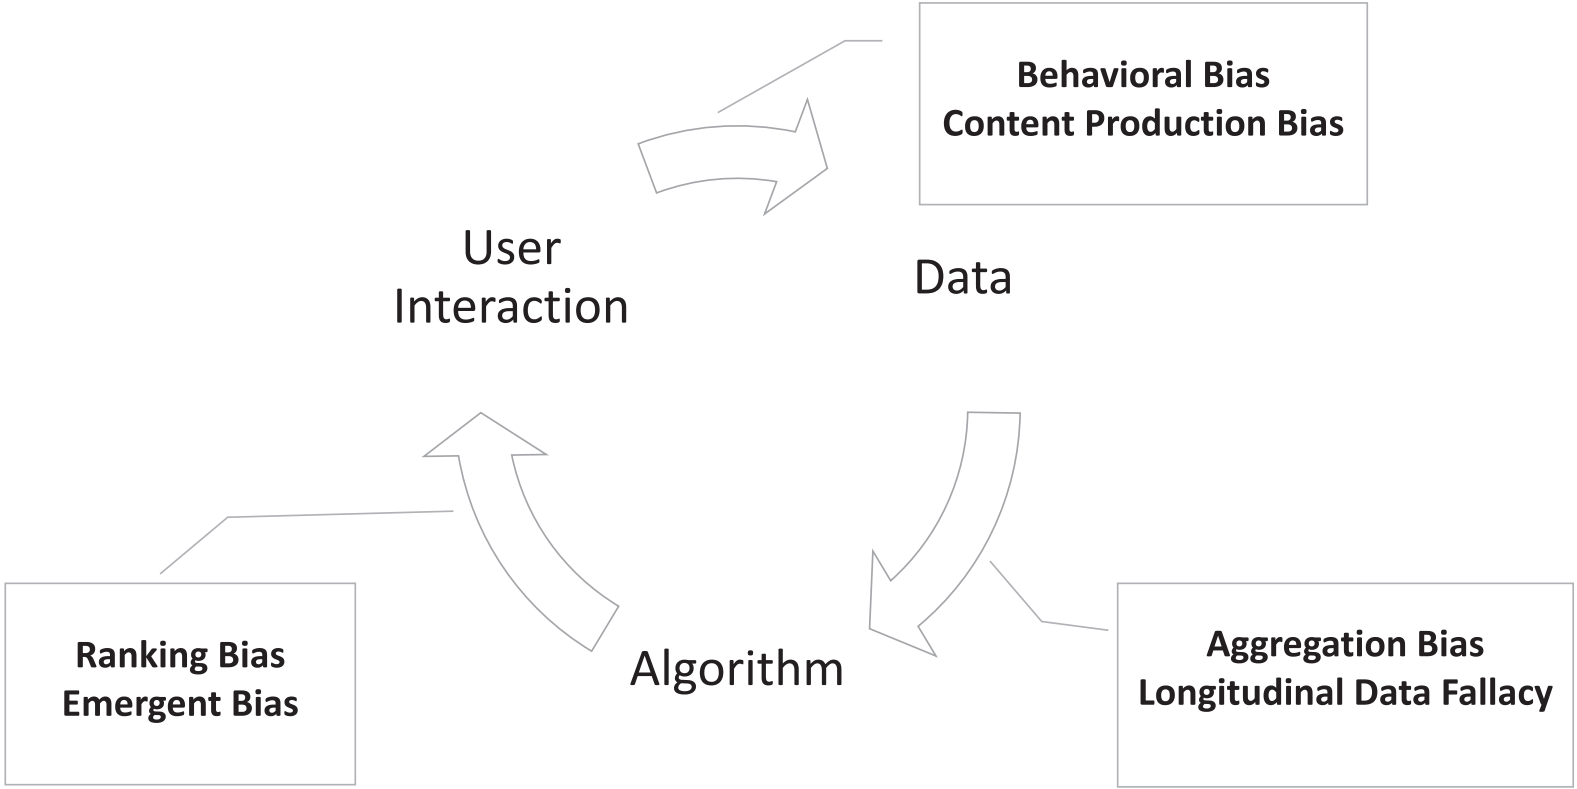
\includegraphics[width=0.8\textwidth]{figures/BiasCategoriesInMLLifecycle.png}
			\caption{Bias definitions in a \gls{ML} lifecycle \autocite{Mehrabi_2021}.}
			\label{fig:bias_definitions_ML_lifecycle}
		\end{figure}
		
		\rawcitationusedstart
		\begin{itemize}
			\item two potential sources of unfairness in machine learning outcomes - those that arise from biases in the data and those that arise from the algorithms ... we observe that biased algorithmic outcomes might impact user experience, thus generating a feedback loop between data, algorithms and users that can perpetuate and even amplify existing sources of bias \autocite{Mehrabi_2021}.
			\item The loop capturing this feedback between biases in data, algorithms, and user interaction is illustrated in Figure 1. We use this loop to categorize definitions of bias in the section below \autocite{Mehrabi_2021}
		\end{itemize}
		\rawcitationusedend
		
		
		\subsection{Bias Types}
		The \autoref{tab:biases_types} aims to provide an overview over what kind of biases exist according to research. The more detailed categories listed in the table try to capture similar kind of biases. This thesis follows roughly the categorization of \textcite{Mehrabi_2021}. Some biases might acctually fit in multiple categories. The definition of the categories including examples of specific biases follows.
		
		\todo{check the c citations in the following chapters}
		
		\begin{table}[H]
			\centering
			\begin{threeparttable}
				\begin{tabularx}{\textwidth}{>{\tblWidthDescription}X|>{\tblWidthContext}X|>{\tblWidthContext}X}
					\toprule
					\textbf{Bias} & \multicolumn{2}{c}{\textbf{Mentioned in Context of}} \\
					& \textbf{\gls{ML}} & \textbf{Dermatology} \\
					%	\midrule
					\multicolumn{3}{l}{\bolditalic{Data Biases}} \\ 
					
					Sampling Biases & X\tnote{1,2,3} & X\tnote{4} \\
					Representation Biases & X\tnote{1} & X\tnote{5,6} \\
					Measurement Biases & X\tnote{1,3} & X\tnote{4,6} \\
					Research Biases & X\tnote{7} & X\tnote{4} \\
					Feature Representation Biases & X\tnote{1,3} & X\tnote{4} \\
					Imaging Biases & & X\tnote{5} \\
					Medical Biases & X\tnote{8} & X\tnote{4} \\
					Temporal Data Biases & X\tnote{1} & X\tnote{4}\\
					
					%	\midrule
					\multicolumn{3}{l}{\bolditalic{Algorithmic Biases}} \\ 
					User-Algorithm Interaction Biases & X\tnote{1} & \\
					External Influence Biases & X\tnote{1} & X\tnote{4} \\
					
					%	\midrule
					\multicolumn{3}{l}{\bolditalic{User Biases}} \\
					Cognitive Biases & X\tnote{1,7} & X\tnote{4} \\
					Behavioral Biases & X\tnote{1,3} & X\tnote{4,5} \\
					Publication Biases &  & X\tnote{4} \\
					Medical Biases & X\tnote{} & X\tnote{4} \\
					
					\bottomrule
				\end{tabularx}
				\begin{tablenotes}
					\footnotesize
					\begin{minipage}{0.33\textwidth}\raggedright
						\item[1] \autocite{Mehrabi_2021}
						\item[2] \autocite{HP_2022}
						\item[3] \autocites{Mester_2022}
					\end{minipage}%
					\begin{minipage}{0.33\textwidth}\raggedright
						\item[4] \autocite{Chakraborty_2024}
						\item[5] \autocite{Young_2020}
						\item[6] \autocite{Montoya_2025}
					\end{minipage}%
					\begin{minipage}{0.33\textwidth}\raggedright
						\item[7] \autocites{Mester_2017}
						\item[8] \autocite{Delgado-Rodriguez_2004}
					\end{minipage}%
				\end{tablenotes}
			\end{threeparttable}
			\caption{Bias categories - grouped according the \gls{ML} lifecycle of \textcite{Mehrabi_2021}}
			\label{tab:biases_types}
		\end{table}
		
		\todo{Feedback Astrid: zu viele Unterkapitel -> anders strukturieren}
		\subsubsection{Data Biases}
		
		\paragraph{Sampling Biases}
		When gathering data, it's usually not possible to gather the data of a whole population. Instead, the data is gathered by sampling. A sample is a subgroup of individuals from the population. To get unbiased results, this sampling process should represent the true population, with a low sampling error \autocites{HP_2022}. This is often achieved with randomized samples. With non-random sampling processes, sampling bias arises. The consequence is, that the insights of one sampled population may not generalize with insights on another sampled popluation \autocite{Mehrabi_2021}.
		
		Those biases can be introduced with a flawed sampling process:
		\begin{itemize}
			\item \textbf{Sampling bias}, due to nonrandom sampling of subgroups, leading to poor generalization \autocite{Mehrabi_2021}
			\item \textbf{Selection bias}, working only on specific subset of the population which is not representative \autocites{Mester_2022}{Chakraborty_2024}
			\item \textbf{Systematic selection bias}, chosen samples differ dramatically from the representative populations; e.g. in dermatology, when only the most severe patient data gets included \autocite{Chakraborty_2024, c5,c6,c33}
			\item \textbf{Ascertainment bias}, tendency to exclude segments from the population due to e.g. cultural differences, such as which patient segment goes to government clinics vs. private clinics (usually influenced by socioeconomic status) \autocite{Chakraborty_2024, c5}
			\item \textbf{Availability bias}, focus on widely available data instead of most representative data \autocites{Chakraborty_2024, c9, c10}{}
			\item \textbf{Survivorship bias}, focus only on pre-selected data, ignoring the initial data-points which got filtered out \autocite{Mester_2022}.
		\end{itemize}
		
		
		\subparagraph{Potential Biases in PASSION}
		PASSION tries to reduce sampling bias in dermatology against high pigmented skin.
		PASSION might introduce (systematic) selection bias or Ascertainment bias, if in the dermatology centers only sickest / more severe patients are seen as indicated by \textcite{Chakraborty_2024}
		PASSION inherits availability bias as it is using \gls{FST} scale.
		Survivorship bias could be relevant for PASSION, if dermatology diseases could be lethal. Further, all patients which are not able to go to one of the dermatology centers which were used in PASSION could be considered to left out by survivorship bias.
		
		\rawcitationstart
		used
		\begin{itemize}		
			\rawcitationusedstart
			\item Sampling Bias. Sampling bias is similar to representation bias, and it arises due to nonrandom sampling of subgroups. As a consequence of sampling bias, the trends estimated for one population may not generalize to data collected from a new population. \autocite{Mehrabi_2021}. This is what the PASSION dataset tries to improve
			
			\item Selection bias - wrong sampling method, working on a specific subset of audience; usually by working only with data that is easy to access \autocites{Mester_2022}{Mester_2017} - statistical bias
			\item Selection bias: Since it is not possible to work with large populations, for most dermatological studies, samples are chosen that are said to be representative of the original population. 
			In selection bias, the selected subgroups are not representative of their original population.
			A variation of this is systematic selection bias, where samples chosen differ dramatically from their representative populations.
			Our experience suggests, such selection bias occurs more commonly in studies conducted in regional referral centers where only the sickest or more severe patients are usually seen.
			For example, a study compared the efficacy of thalidomide vs. prednisolone in hospitalised patients of erythema nodosum leprosum. It derived that thalidomide was more efficacious than steroids in erythema nodosum leprosum. Such findings cannot be generalised to all erythema nodosum leprosum since patients admitted to a regional referral center will likely have more severe disease.5,6,33 \autocite{Chakraborty_2024}
			\item  Availability bias: More emphasis is placed on widely available data than scantily available data. A classic example is the use of antihistamines in pregnancy dermatoses, where nearly all standard books recommend first-generation antihistamine chlorpheniramine because more data is available.9 10. \autocite{Chakraborty_2024} - dermatology
			
			\item Survivorship bias \autocites{Mester_2022}{Mester_2017} - statistical bias
			
			
			\item Ascertainment Bias: This bias is commonly encountered in venereology practice. It is defined as a bias due to the tendency of some segments of the target population to get excluded due to cultural and other differences. For example, in most venereology clinics in government setups, studies show that venereal diseases are commoner in lower socioeconomic status. One reason might be that the higher socioeconomic status people tend to go to private practitioners and thereby get excluded from government-run clinics.9,10 Allocation concealment and blinding are good ways to avoid this. 5. \autocite{Chakraborty_2024} - healthcare
			\rawcitationusedend
		\end{itemize}
		
		even more extensive
		\begin{itemize}
			\item Selection bias is again divided into two types endogenous selection bias and exogenous selection bias. The best example of endogenous selection bias in dermatology is the inclusion of non-response. If a trial tests the efficacy of a particular biologic in psoriasis, the response is usually collected from trial participants via postal services. Certain participants will not respond, although they might have substantially improved. Their exclusion will result in significant differences in efficacy evaluation.33
			Exogenous selection bias results when both treatment and outcome result from dependency on an external variable that is not controlled. For example, if sunlight exposure is not controlled, it will influence both the intervention and control groups since psoriasis is a photosensitive (and photoexcerbated) dermatosis. \autocite{Chakraborty_2024} - dermatology
			
			
			\item survivorship bias - World War II planes \autocite{Silfwer_2017} - https://doctorspin.org/media-psychology/psychology/survivorship-bias/
		\end{itemize}
		
		\rawcitationend
		
		\paragraph{Representation Biases}
		\todo{still describe this category} 
		
		Those biases can be introduced :
		\begin{itemize}
			\item \textbf{Representation bias}, non-representative sample lead to missing subgroups or other representation anomalies, which can be harmful to downstream applications. Popular \gls{ML} datasets suffer from representation bias \autocites{Mehrabi_2021}{M142_Shankar_2017}
			\item \textbf{Population Bias}. Population bias arise when statistics, demographics and characteristics in the sample differ from the target population \autocite{M120_Olteanu_2019}. The data it creates is non-representative for the target population \autocite{Mehrabi_2021}.
			\item \textbf{Aggregation bias} occurs, when "false conclusions are drawn about individuals from observing the entire population". It doesn't matter, whether the subgroups are represented equally in the training set, any generalized assumptions can result in aggregation bias \autocite{Mehrabi_2021}. In medicine, diseases can present themselves differently across genders and ethnicities \autocite{M144_Suresh_2021}. Therefore, diagnostic models need to incorporate those differences to mitigate aggregation bias \autocite{Mehrabi_2021}.
			\item \textbf{Simpson's Paradox} is a type of aggregation bias, which arises in heterogeneous data analysis. Observed associations disappear or reverses in the subgroup data \autocite{Mehrabi_2021}.
		\end{itemize}
		
		
		\subparagraph{Potential Biases in PASSION}
		PASSION tries to mitigate representation bias, by including more FST skin types - however, it could introduce other representation biases
		Aggregation bias and Simpson's Paradox could potentially be an issue when the analyzed skin diseases present themselves differently in patients based on their genetics
		
		
		\rawcitationstart
		used
		\begin{itemize}		
			\rawcitationusedstart
			\item Representation Bias. Representation bias arises from how we sample from a population during data collection process \autocite{M144_Suresh_2021}. Non-representative samples lack the diversity of the population, with missing subgroups and other anomalies \autocite{Mehrabi_2021}.
			\item Popular machine-learning datasets that serve as a base for most of the developed algorithms and tools can also be biased—which can be harmful to the downstream applications that are based on these datasets. ... In \autocite{M142_Shankar_2017}, researchers showed that these datasets suffer from representation bias and advocate for the need to incorporate geographic diversity and inclusion while creating such datasets. \autocite{Mehrabi_2021}
			
			\item Population Bias. Population bias arises when statistics, demographics, representatives, and user characteristics are different in the user population of the platform from the original target population \autocite{M120_Olteanu_2019}. Population bias creates non-representative data. ... More such examples and statistics related to social media use among young adults according to gender, race, ethnicity, and parental educational background can be found in \autocite{M64_Hargittai_2007}. \autocite{Mehrabi_2021}
			
			\item Aggregation Bias. Aggregation bias (or ecological fallacy) arises when false conclusions are drawn about individuals from observing the entire population. An example of this type of bias can be seen in clinical aid tools. Consider diabetes patients who have apparent morbidity differences across ethnicities and genders. Specifically, HbA1c levels, that are widely used to diagnose and monitor diabetes, differ in complex ways across genders and ethnicities. Therefore, a model that ignores individual differences will likely not be well-suited for all ethnic and gender groups in the population \autocite{M144_Suresh_2021}. This is true even when they are represented equally in the training data. Any general assumptions about subgroups within the population can result in aggregation bias. \autocite{Mehrabi_2021}. --> could also be important for dermatology issues!!!
			\begin{itemize}
				\item Simpson’s Paradox. Simpson’s paradox is a type of aggregation bias that arises in the analysis of heterogeneous data [18]. The paradox arises when an association observed in aggregated data disappears or reverses when the same data is disaggregated into its underlying subgroups (Fig. 2(a)). ... After analyzing graduate school admissions data, it seemed like there was bias toward women, a smaller fraction of whom were being admitted to graduate programs compared to their male counterparts. However, when admissions data was separated and analyzed over the departments, women applicants had equality and in some cases even a small advantage over men. The paradox happened as women tended to apply to departments with lower admission rates for both genders. Simpson’s paradox has been observed in a variety of domains, including biology [37], psychology [81], astronomy [109], and computational social science [91].\autocite{Mehrabi_2021}.
			\end{itemize}
		\end{itemize}
		\rawcitationusedend
		\rawcitationend
		
		\paragraph{Measurement Biases}
		How features are chosen, used and measured can lead to biases \autocites{Mehrabi_2021}{M144_Suresh_2021}.
		
		Examples for such biases are:
		\begin{itemize}
			\item \textbf{Measurement bias} in general, e.g. using mismeasured \glspl{proxyVar} lead to misinterpretations of the outcome \autocite{Mehrabi_2021}
			
			\item \textbf{Observer bias} is a subconscious bias which can occur in different forms. Either, researchers projects their own expectations on the research and influence the testers accordingly \autocite{Mester_2022}. In other cases, different observes report the same observation differently \autocite{Chakraborty_2024, c29, c26}
			
			\item \textbf{Annotator bias} is a special form of observer bias. The labeling process of human annotators can be influenced by lots of factors (e.g. personal background, social context) and even minor design choices (e.g. scale order, image context). This can introduce inconsistencies when labeling the data \autocite{Montoya_2025}
			
			\item \textbf{Recall bias}. This bias occurs when queried individuals do not remember things correctly, due to humans selective memory. This can cause misinterpretation, for example when analyzing causes and effects of behaviour on certain diseases in medicine \autocites{Mester_2022}{Chakraborty_2024, c3-6, c2}.
		\end{itemize}
		
		\subparagraph{Potential Biases in PASSION}
		Measurement Bias (proxy var) - Country of Origin in PASSION depending on the interpretation - should not be used for ethnicity, as this is not linked directly to the genes, see example https://medium.com/bcggamma/practice-ai-responsibly-with-proxy-variable-detection-42c2156ad986
		
		Annotator bias regarding skin tone labeling has been investigated in \autocite{Montoya_2025}. PASSION should evaluate its process.
		
		
		\rawcitationstart
		used
		\begin{itemize}		
			\rawcitationusedstart
			\item Measurement Bias. Measurement, or reporting, bias arises from how we choose, utilize, and measure particular features \autocite{M144_Suresh_2021} (e.g. mismeasured proxy variables) \autocite{Mehrabi_2021}. (= e.g. someone who lives at that postal code probably has this ethnicity ); --> could that be an issue with the country of origin feature?
			
			\item This study found that while using skin tone instead of race for fairness evaluations in computer vision seems objective, the annotation process remains biased by human annotators. Untested scales, unclear procedures, and a lack of awareness about annotator backgrounds and social context significantly influence skin tone labeling. This study exposes how even minor design choices in the annotation process, like scale order (dark to light instead of light to dark) or image context (face or no face, skin lesion presence), can sway agreement and introduce uncertainty in skin tone assessments. ... The researchers emphasize the need for greater transparency, standardized procedures, and careful consideration of annotator biases to mitigate these challenges and ensure fairer and more robust evaluations in computer vision. \autocite{Montoya_2025} - demographic dermatology bias
			
			\item Observer bias - projecting expectations onto the research \autocites{Mester_2022}{Mester_2017} - statistical bias
			\item  Observer bias: When different observers view the same observation, they report it differently e.g., different observers may give differing descriptions about subtle features in the histopathology report of a skin biopsy.29 26. \autocite{Chakraborty_2024} - dermatology
			
			\item Recall bias - respondent doesn't remember things correctly; Recall bias is another common error of interview/survey situations. It happens when the respondent doesn’t remember things correctly. It’s not about bad or good memory – humans have selective memory by default. After a few years (or even a few days), certain things stay and others fade. It’s normal, but it makes research much more difficult. \todo{keep an eye on this when recalling evidences!!}
			\autocites{Mester_2022}{Mester_2017} - statistical bias
			\item Memory or recall bias: This is a type of bias where sufferers of a disease, often termed cases, have a greater tendency to recall a particular habit than non-sufferers, viz controls. This results in an uneven distribution of risk factors between the cases and controls. An example of this would be a case-control study to evaluate the association between dental amalgam use and the development of oral lichen planus. Those with lichen planus are more likely to recall a history of dental amalgam use than those who do not have the disease. This difference in recall between a diseased cohort and control has resulted in difficulties in assessing the association between diet and many dermatological diseases – like milk and chocolate consumption and acne, fatty meals and psoriasis, sugary meals and psoriasis, agricultural exposure to insecticides and pemphigus and so on.3–6 2. \autocite{Chakraborty_2024} - dermatology
			
			\rawcitationusedend
		\end{itemize}
		\rawcitationend
		
		\paragraph{Research Biases}
		\todo{consider to move at beginning / out of data biases}
		Researchers and their processes can also be biased in multiple ways:
		\begin{itemize}
			\item \textbf{Funding / Sponsorship bias}, when a study is deliberately supporting those findings, which the sponsor expects \autocites{Chakraborty_2024, c22}{Mester_2017}
			
			\item \textbf{Data dredging bias}. The statistical methods and model are chosen to provide a certain p-value, to improve the probability of the research hypothesis being true. \todo{consider to move this to an own reporting section} \autocite{Chakraborty_2024}
			
			\item \textbf{Hypothetical bias}. Hypothetical questions lead to responses that do not reflect, what interviewees would do in real life. \autocite{Chakraborty_2024, c31, c28} \todo{isn't this a user bias instead?}
		\end{itemize}
		
		\subparagraph{Potential Biases in PASSION}
		Since the PASSION dataset is already published, the research biases might already be introduced. It is not feasible during the duration of this thesis to make an evaluation on those biases. Instead, I would recommend the PASSION team and researcher in general, to check the list above carefully and take measures against them. Maybe, an external evaluation could help to detect and prevent those biases even better.
		
		
		
		\rawcitationstart
		used
		\begin{itemize}		
			\rawcitationusedstart
			\item Funding bias \autocites{Mester_2022}{Mester_2017} - statistical bias
			\item  Industry sponsorship bias: This has now been reclassified as conflict-of-interest bias. In short, the study deliberately supports the findings expected from it by its sponsors. 22.\autocite{Chakraborty_2024} - dermatology
			
			Reporting biases
			\item  Data dredging bias: It is an entirely avoidable bias. This is subdivided into two types – Fishing type and “P-value hacking” type. It involves using multiple statistical methods to get the desired p-value and selecting the statistical model that gives the p-value the author wants. This is “lamentably common” in dermatological research.16 To detect data dredging bias, always perform a “p-curve analysis” while performing a meta-analysis.17,18 Much emphasis is nowadays given to the confidence interval instead of the p-value, which gives an approximate idea of the range in which one can be 95\% (or 90\%, depending on the confidence interval chosen) sure that the result is correct. The confidence interval remains unaffected by p-value dredging. This subject has been reviewed in depth in recent works.18,19 15.\autocite{Chakraborty_2024}
			
			\item Hypothetical bias: Many dermatological researches (and some life quality questionnaires like vitiQoL) use hypothetical questions – like “What would you do when some stranger asks you about your lesion?”. The responses to these questions by the study participants often do not tally with what they would do in real life. This is called hypothetical bias and is avoided by adopting the ex-ante approach.31 28. \autocite{Chakraborty_2024} - dermatology
			\rawcitationusedend
		\end{itemize}
		\rawcitationend
		
		\paragraph{Feature Representation Biases}
		
		Some of those biases are:
		\begin{itemize}
			\item \textbf{Omitted Variable Bias} arises when variables are not included in the model, which leads to situations for which the model is not ready for \autocites{Mehrabi_2021}{Mester_2022}\autocites{M38_Clarke_2005}{M131_Riegg_2008}\autocite{M114_Mustard_2003}.
			\item \textbf{Collider Bias} Two variables can influence a common third variable, the collider variable. When sampling is restricted by this collider variable, it could lead to a distortion  \autocite{Chakraborty_2024, c4,c8,c9}.
		\end{itemize}
		
		
		\subparagraph{Potential Biases in PASSION}
		The ethnicity is omitted in the PASSION dataset which could lead to issues
		See the medical section for more specific collider bias, maybe there could be others
		
		\rawcitationstart
		used
		\begin{itemize}
			\rawcitationusedstart
			\item Omitted Variable Bias. Omitted variable bias4 occurs when one or more important variables are left out of the model \autocites{M38_Clarke_2005}{M131_Riegg_2008}\autocite{M114_Mustard_2003}. Something that the model was not ready for\autocite{Mehrabi_2021}. did not take into account \autocite{Mehrabi_2021}
			\item Omitted variable bias \autocites{Mester_2022}{Mester_2017} - statistical bias
			\item Collider Bias: This is an under-appreciated bias, and often confused with a confounder. This is especially seen in observational studies where it is defined as a distortion produced by the restriction of sampling by a collider variable. A collider variable is defined as one that has an independent effect on the outcome studied apart from the studied variable. In simpler terms, collider bias occurs when exposure and development influence a common third variable. That variable or collider is controlled by study design or in the analysis. An example is the observation that psoriasis patients tend to have more depression and anxiety disorders. Since severe psoriasis patients tend to get hospitalised and also get screened for mental health issues, a spurious association between them could have been obtained due to collider bias. The two variables viz psoriasis and depression converged, i.e., collided, into a single outcome – hospitalization.8,9 4. \autocite{Chakraborty_2024} - dermatology
			\rawcitationusedend
		\end{itemize}
		\rawcitationend
		
		
		\paragraph{Imaging Biases}
		Dealing with images can lead to a whole other set of challenges, which can lead to biases. The challenges are for example technical variations in hardware and software but also differences in how images are gathered or what is in it \autocite{Young_2020}.
		
		Those biases can be introduced :
		\begin{itemize}
			\item \textbf{Image Quality Bias}. The quality of an image (zoom level, focus, lightning) could be associated with the classification \autocite{Young_2020}
			\item \textbf{Visual Artifact Bias}. Other artifacts, such as presence of hair or surgical ink markings on dermatology images, can decrease classification performance \autocite{Winkler et al., 2019 & Bisla et al., 2019 (from Young_2020)}
			\item \textbf{Field of View Bias}. What view is captured in the image can interfere with prediction quality  what is it, consequence \autocite{Mishra et al., 2019 from Young_2020}
		\end{itemize}
		
		
		\subparagraph{Potential Biases in PASSION}
		The PASSION model could learn to associate unrelated visual effects, hair, body parts or image quality with a disease.
		
		
		\rawcitationstart
		used
		\begin{itemize}		
			\rawcitationusedstart
			\item Image quality. Several barriers to \gls{AI} implementation in the clinic need to be overcome with regards to imaging (Figure 1). These include technical variations (e.g., camera hardware and software) and differences in image acquisition and quality (e.g., zoom level, focus, lighting, and presence of hair). For example, the presence of surgical ink markings is associated with decreased specificity (Winkler et al., 2019), field of view can significantly affect prediction quality (Mishra et al., 2019), and classification performance improves when hair and rulers are removed (Bisla et al., 2019). We have developed a method to measure how model predictions might be biased by the presence of a visual artifact (e.g., ink) and proposed methods to reduce such biases (Pfau et al., 2019). Poor quality images are often excluded from studies, but the problem of what makes an image adequate is not well studied. Ideally, models need to be able to express a level of confidence in a prediction as a function of image quality and appropriately direct a user to retake photos if needed. \autocite{Young_2020} - dermatology
			\rawcitationusedend
		\end{itemize}
		\rawcitationend
		
		\paragraph{Medical Biases}
		In \gls{ML} for health care, there are special medical versions of the mentioned biases as well as completely new biases. They require special attention, since they directly influence the diagnosis or treatment of a disease.
		
		Those biases can be introduced:
		\begin{itemize}
			\item \textbf{Berkesonian bias} occurs in hospital-based studies when two variables influence hospital or clinical attendance independently. This can lead to a distorted estimation of the relationship between those variables because the study population of hospitalized patients is not representative of the whole population \autocite{Chakraborty_2024, c3, c7}
			\item \textbf{Informed presence bias}, the probability to get screened for other diseases is higher for people who seek medical care. Like Berkesonian bias, this can lead to misleading interpretations of relationships between two diseases \autocite{Chakraborty_2024, c27, c23}
			\item \textbf{Diagnostic access bias}, depending on the geographical location, individuals have better access to medical care. Therefore, their disease prevalence could appear to be higher and diseases could be diagnosed earlier. \autocite{Chakraborty_2024, c19-c21}
			\item \textbf{Diagnostic reference test bias} is a \textbf{verification bias}, where not all individuals receive the same reference test for the diagnostic process, potentially leading to different diagnoses. \autocite{Chakraborty_2024, c21}
			\item \textbf{Mimicry bias}, exposures to treatment options can cause a disease which presents itself similar to the study disease, which potentially creates misleading data \autocite{Chakraborty_2024, c28, c25}
			\item \textbf{Unacceptable Disease bias}. When a disease is socially unacceptable, it can result in under-reporting of the same disease \autocite{Chakraborty_2024, c30, c27}
			\item \textbf{Healthy volunteer selection bias}, is a type of self-selection bias where the volunteers are in general healthier than the population due to more interest in health \autocite{Delgado-Rodriguez_2004}
		\end{itemize}
		
		\subparagraph{Potential Biases in PASSION}
		Berkesonian bias depending on the chosen hospitals
		Informed presence bias regarding correlation between impedigo and the other diseases
		Diagnostic access bias can somewhat be addressed by PASSION, since its dataset includes samples of later states of diseases. However, in the PASSION context itself, this bias could still be relevant.
		Diagnostic reference test bias could be inherited in the PASSION dataset, depending on how the dermatologists work.
		Mimicry bias is not relevant regarding the exposures since PASSION does not hold any exposure data. However, diseases which mimicry others could lead to issues if they are not detected.
		
		
		
		\rawcitationstart
		used
		\begin{itemize}		
			\rawcitationusedstart
			\item Berkesonian Bias: Named after Dr. Joseph Berkeson, this bias reflects the variation in rates of hospital admission or clinic attendance for different diseases. For example, if a study is conducted to know the effect of pregnancy on syphilis in an antenatal clinic, we are likely to get biased data since the two conditions, viz pregnancy and syphilis, are both likely to affect clinic attendance and all observations related to the relationship between pregnancy and syphilis.7 3. \autocite{Chakraborty_2024} - dermatology
			
			\item  Informed presence bias: Simply, a person attending a health center is more likely to get screened for other unrelated comorbidities than those not attending a health center e.g., the finding psoriasis is associated with depression has now been criticised because those having psoriasis also have a greater chance to be screened for depression since they are already attending a health center.27 23. \autocite{Chakraborty_2024} - dermatology	
			
			\item  Diagnostic Access Bias: Individuals in certain geographical localities have better access to medical care and, hence, may appear to have higher disease prevalence. For example, atopic dermatitis is believed to be commoner in the West – this could be due to better and earlier diagnostic facilities available than in India.19,20 17.\autocite{Chakraborty_2024}
			
			\item  Diagnostic reference test bias: These bias results when all individuals do not receive the same reference test. e.g., direct immunofluorescence studies may not be done for all patients with pemphigus vulgaris some patients may receive only a skin biopsy-based diagnosis. It is a subtype of verification bias. Another variation of this type of bias is partial reference bias, where only some of the study participants receive the index and the reference tests.21\autocite{Chakraborty_2024}
			
			\item  Mimicry bias: When an exposure causes a disease that resembles the study disease, mimicry bias can result. For example, certain drugs are known to cause a pityriasis rosea-like reaction, which, although looks like pityriasis rosea, differs from it.28 25.\autocite{Chakraborty_2024} - dermatology
			
			\item Unacceptable disease bias: This occurs in socially unacceptable diseases like leprosy and STDs, which result in under-reporting.30 27. \autocite{Chakraborty_2024} - dermatology
			
			\item \todo Other such studies were conducted in [\autocite{M54_Fry_2017}] which states that UK Biobank, a large and widely used genetic dataset, may not represent the sampling population. Researchers found evidence of a “healthy volunteer” selection bias. [150] has other examples of studies on existing biases in the data used in the medical domain. [157] also looks at machine-learning algorithms and data utilized in medical fields, and writes about how artificial intelligence in health care has not impacted all patients equally.\autocite{Mehrabi_2021} --> [150] also provides an ovverview over the impact of social determinants on health, such as Economic stability, neighborhood and physical environment, education, food, community and scial context, access to healthcare and quality
			\item The healthy volunteer effect is a particular case: when the participants are healthier than the general population. \autocite{Delgado-Rodriguez_2004}
			\rawcitationusedend
		\end{itemize}
		\rawcitationend
		
		\paragraph{Temporal Biases}
		Differences in populations and their behaviour over time can lead to temporal biases \autocite{M120_Olteanu_2019}.
		Certain studies require to track temporal data, to learn about their behaviour over time. Disease progression is also a factor measured over time \autocite{Mehrabi_2021}. For PASSION, temporal biases are currently irrelevant, since PASSION contains images independently of time and is not tracking the disease progression. Therefore, the listed biases in this chapter are not explained in detail, refer to the sources for further information.
		
		Examples for temporal data biases are:
		\begin{itemize}
			\item \textbf{Longitudinal Data Fallacy} \autocite{Mehrabi_2021}
			\item \textbf{Chronological bias} \autocite{Chakraborty_2024, c9, c13}
			\item \textbf{Immortal time bias} \autocite{Chakraborty_2024, c24, c20}
		\end{itemize}
		
		
		\todo{added until here}
		\subsection{Algorithmic Biases}
		When an algorithm adds biases to unbiased input data one speaks of \textbf{Algorithmic Bias} \autocite{M9_Baeza-Yates_2018}. This could occur due to algorithmic design choices like optimization functions, regularizations and statistically biased estimators \autocite{M44_Danks_2017}.
		
		\rawcitationstart
		used
		\begin{itemize}		
			\rawcitationusedstart
			\item Algorithmic Bias. Algorithmic bias is when the bias is not present in the input data and is added purely by the algorithm \autocite{M9_Baeza-Yates_2018}. The algorithmic design choices, such as use of certain optimization functions, regularizations, choices in applying regression models on the data as a whole or considering subgroups, and the general use of statistically biased estimators in algorithms \autocite{M44_Danks_2017}, can all contribute to biased algorithmic decisions that can bias the outcome of the algorithms.\autocite{Mehrabi_2021}.
			\rawcitationusedend
		\end{itemize}
		\rawcitationend
		
		\paragraph{User Algorithm Interaction Biases}
		\begin{itemize}
			\item \textbf{User Interaction Bias}. This biases can be triggered by the user interface or the user themselves. The user interface influences the user to behave in a certain way, which could introduce bias in the user behaviour. Users impose this (or their own) biased behavior through interaction on the algorithm \autocite{M9_Baeza-Yates_2018}. \textbf{Presentation bias} and \textbf{Ranking bias} are further subtypes mentioned by \textcites{M93_Lerman_2014}{Mehrabi_2021}.
			\item \textbf{Emergent Bias}. When real users interact with an algorithm, this bias arises some time after the design was completed due to changes in population. It appears more likely in user interfaces \autocite{M53_Friedman_1996}.
		\end{itemize}
		
		
		\subparagraph{Potential Biases in PASSION}
		The user interaction biases, especially the emergent bias could potentially become an issue for PASSION, when the project starts to become publicly available \gls{teledermatology}. Also, the interface design should be evaluated, so that no presentation or ranking bias gets introduced.
		
		\rawcitationstart
		used
		\begin{itemize}		
			\rawcitationusedstart
			\item Emergent Bias. Emergent bias occurs as a result of use and interaction with real users. This bias arises as a result of change in population, cultural values, or societal knowledge usually some time after the completion of design \autocite{M53_Friedman_1996}. This type of bias is more likely to be observed in user interfaces, ... This type of bias can itself be divided into more subtypes, as discussed in detail in \autocite{M53_Friedman_1996}. \autocite{Mehrabi_2021}. probably less relevant at the first stage
			
			\item User Interaction Bias. User Interaction bias is a type of bias that can not only be observant on the Web but also get triggered from two sources—the user interface and through the user itself by imposing his/her self-selected biased behavior and interaction \autocite{M9_Baeza-Yates_2018}. This type of bias can be influenced by other types and subtypes, such as presentation and ranking biases. \autocite{Mehrabi_2021}. -- more relevant for later, when the application would become bigger
			\rawcitationusedend
			\begin{itemize}
				\item Presentation Bias. Presentation bias is a result of how information is presented \autocite{M9_Baeza-Yates_2018} (can only click on content they see, could be the case that user does not see all info on web) \autocite{Mehrabi_2021}.
				\item Ranking Bias. The idea that top-ranked results are the most relevant and important will result in attraction of more clicks than others. This bias affects search engines \autocite{M9_Baeza-Yates_2018} and crowdsourcing applications \autocite{M93_Lerman_2014}.\autocite{Mehrabi_2021}.
			\end{itemize}
		\end{itemize}
		\rawcitationend
		
		\paragraph{External Influence Biases}
		
		Those biases can be introduced :
		\begin{itemize}
			\item \textbf{Evaluation Bias}. When inappropriate or disproprtionate benchmarks are used in model evaluation, they can introduce the benchmarks biases into the model. \autocites{M144_Suresh_2021}{M24_Buolamwini_2018}
			
			\item  \textbf{Incorporation bias}. When index tests in diagnostic accuracy studies are part of the reference tests, this results in elevated sensitivity for the index tests \autocites{Chakraborty_2024, c21, c25, c26}{Young_2020}.
			
			\item \textbf{Popularity Bias}. More popular items tend to be exposed more. Popularity metrics can be manipulated though or not reflecting good quality, this can lead to bias \autocites{M117_Ciampaglia_2018}{Mehrabi_2021}.
			
			\item \textbf{Generalization Issues}.  \autocite{} \todo{add those from young}
		\end{itemize}
		
		
		\subparagraph{Potential Biases in PASSION}
		\todo{add}
		
		\rawcitationstart
		used
		\begin{itemize}		
			\rawcitationusedstart
			\item Evaluation Bias. Evaluation bias happens during model evaluation \autocite{M144_Suresh_2021}. This includes the use of inappropriate and disproportionate benchmarks for evaluation of applications such as Adience and IJB-A benchmarks. These benchmarks are used in the evaluation of facial recognition systems that were biased toward skin color and gender \autocite{M24_Buolamwini_2018}, and can serve as examples for this type of bias \autocite{M144_Suresh_2021}. \autocite{Mehrabi_2021}. -- important for this thesis
			
			\item  Incorporation bias: This is principally relevant for diagnostic accuracy studies when the index test forms a part of the reference test, resulting in elevated sensitivity e.g., if one wants to compare the grattage test vs. dermoscopy in psoriasis and does dermoscopy only from areas of grattage positivity, one would get a very high sensitivity for the grattage test because it was incorporated into the reference test, i.e., dermoscopy.25,26 21.\autocite{Chakraborty_2024}
			
			\item Popularity Bias. Items that are more popular tend to be exposed more. However, popularity metrics are subject to manipulation—for example, by fake reviews or social bots \autocite{M117_Ciampaglia_2018}. ... this presentation may not be a result of good quality; instead, it may be due to other biased factors. \autocite{Mehrabi_2021}.
			\rawcitationusedend
		\end{itemize}
		\rawcitationend
		
		
		\subsection{User Biases}
		
		\paragraph{Cognitive Biases}
		Biases which are related to human perception belong to the category of cognitive biases. They are affecting how data should be presented and interpreted \autocite{Mester_2017}
		
		Those biases can be introduced :
		\begin{itemize}
			\item \textbf{Confirmation Bias}. When people have pre-conceptions, they will only listen to the part of presented information which reinforce those "facts", regardless whether the facts are true or not \autocite{Mester_2017}. In health-care, this can be observed when patients report increases in diseases due to potentially nonfactual information they found on the internet \autocite{Chakraborty_2024, c15, c14}.
			\item \textbf{Belief Bias}. A stronger version of the confirmation bias: Someone who is affected by this bias is so sure about their own gut feelings that they will ignore results of a data research project \autocite{Mester_2017}.
			\item \textbf{Previous Opinion Bias}. When performing multiple tests, the knowledge about the outcome of the previous tests probably influences the results \autocite{Chakraborty_2024}
			\item \textbf{Cause-Effect Bias}. The famous senctence "correlation does not imply causation" can be used here - when correlation between two variables is misinterpreted as a cause-effect in the wrong direction, this bias applies  \autocite{Mester_2017}
			\item \textbf{Historical Bias}. Preexisting biases in the world can affect the data generation process \autocite{M144_Suresh_2021}. Even if they reflect the current reality, it is worth to consider whether those biases should affect the algorithms in question \autocite{Mehrabi_2021}.
			\item \textbf{Content Production Bias}. User generated contents can introduce biases by systematical differences in the production process, stucture and appearance, which might stem from the users background \autocite{M120_Olteanu_2019}.
		\end{itemize}
		
		\subparagraph{Potential Biases in PASSION}
		For PASSION, confirmation bias could lead to issues in the initial diagnosis and could therefore lead to biased data labeling. Same with the previous opinion bias. The later can be reduced when it is ensured, that the labeling experts are diagnosing the diseases independently of each other, so that they do not know the previous opinions.
		Cause-Effect bias is lesser an issue for PASSION, since the causes of the diseases are not analyzed. It could more be an inherit problem, that the algorithm learns wrong causes for diseases, such as appearing hair
		Historical bias can affect PASSIONs process in various ways.
		In PASSION context, Content Production Bias could have an impact on how the images are taken.
		
		
		\rawcitationstart
		used
		\begin{itemize}		
			\rawcitationusedstart
			\item  	
			\item Cognitive bias \autocites{Mester_2017} - statistical bias
			
			\item  Previous opinion bias: In performing a second diagnostic test, if the result of a previous test is known, it is likely to influence the result. An extension of this is the Greenwald’s law of lupus: the Sontheimer amendment – anything and everything that happens to a lupus erythematosus patient is correctly or incorrectly attributed to lupus.32 29. \autocite{Chakraborty_2024} - dermatology
			
			\item  Confirmation bias: This bias occurs when study participants have a preconceived notion of their disease that may not be based on facts. For example, we have observed that in North India many tinea patients report an increase in their disease due to taking meat, fish, and other so-called “hot foods”. They may also present information they have collected from the internet which reinforces their beliefs.15 14.\autocite{Chakraborty_2024} - dermatology
			
			\item Cause-effect bias \autocites{Mester_2022}{Mester_2017} - statistical bias
			
			
			\item Historical Bias. Historical bias is the already existing bias and socio-technical issues in the world and can seep into from the data generation process even given a perfect sampling and feature selection \autocite{M144_Suresh_2021}. ... search results were of course reflecting the reality, but whether or not the search algorithms should reflect this reality is an issue worth considering \autocite{Mehrabi_2021} - maybe relevant
			
			\item Content Production Bias. Content Production bias arises from structural, lexical, semantic, and syntactic differences in the contents generated by users \autocite{M120_Olteanu_2019}. \autocite{Mehrabi_2021} -- could the quality of the pictures been related to this as well?	
			\rawcitationusedend
		\end{itemize}
		\rawcitationend
		
		\paragraph{Behavioral Biases}
		
		Those biases can be introduced :
		\begin{itemize}
			\item \textbf{Behavioral Bias}. User behaviour can differ depending on the platforms, contexts, cultures, or datasets \autocite{M120_Olteanu_2019}.
			\item \textbf{Self-Selection Bias}. This subtype of selection bias occurs when study participants can select themselves. Less proactive people, people with less time or interest will be excluded or underrepresented \autocites{Mester_2022}{Mehrabi_2021}. \textbf{Non-Responder bias} is a subtype, where part of the population is not responding e.g. to fill out a survey or post-study responses queried by postal services \autocite{Chakraborty_2024}. \todo{maybe categorize this in the data biases or the healthy volunteer bias here}
			\item \textbf{Social Bias}. When the actions of others affect our judgment, it is called social bias. For example ratings in juries can be affected by this \autocite{M9_Baeza-Yates_2018}.
		\end{itemize}
		
		
		\subparagraph{Potential Biases in PASSION}
		For PASSION the behavioral biases can affect who is going to the dermatologists for what reasons. Therefore, the approach to use data from different countries may be benefitial, since potentially the cultural differences could differ.
		Self-selection is an issue, since only those patients can be included in the database which go to the hospitals.
		
		
		
		\rawcitationstart
		used
		\begin{itemize}		
			\rawcitationusedstart
			\item Self-Selection Bias. Self-selection bias4 is a subtype of the selection or sampling bias in which subjects of the research select themselves. \autocite{Mehrabi_2021}
			\item Self-selection bias - when you let the subjects of the analyses select themselves, less proactive people will be excluded \todo{could be an issue as well for PASSION, couldn't it? since the doctors probably ask the clients. One way to go is to default should be to provide access to the data. but is it ethical?} \autocites{Mester_2022}{Mester_2017}- statistical bias
			A variation of this is non-responder bias, where non-responders to a questionnaire differ significantly from responders.9 9. \autocite{Chakraborty_2024} - dermatology
			
			\item Social Bias. Social bias happens when others’ actions affect our judgment \autocite{M9_Baeza-Yates_2018}. (case where we want to rate or review an item with a low score, but when influenced by other high ratings, we change our scoring thinking that perhaps we are being too harsh [\autocite{M9_Baeza-Yates_2018}, \autocite{M151_Wang_2014}.) \autocite{Mehrabi_2021}
			
			\item Behavioral Bias. Behavioral bias arises from different user behavior across platforms, contexts, or different datasets \autocite{M120_Olteanu_2019}. \autocite{Mehrabi_2021} maybe, people from different countries go to the dermatologist for different diseases, based on cultural differences?
			\rawcitationusedend
			
		\end{itemize}
		\rawcitationend
		
		\paragraph{Publication Biases}
		
		Those biases can be introduced :
		\begin{itemize}
			\item \textbf{Publication Bias}
			\item \textbf{Hot stuff bias} is a subtype of publication bias, where Journals are less critical about trending topics, which lead to more frequent publishing of those topics. This in turn can lead to flawed meta-analyses regarding those topics  \autocite{Chakraborty_2024, c22, c23, c19}.
			\item \textbf{All is Well Bias}. This bias is a different view on the hot stuff bias. Theories which align with the view of the majority are more likely to be pubhlished than an opposing view \autocite{Chakraborty_2024, c7,c10-12}.
			\item \textbf{Rethoric Bias}. Charismatic writing or when the press is more vocal about findings can lead to greater influence over individuals than other available facts \autocite{Chakraborty_2024}.
			\item \textbf{Novelty Bias}. Newer interventions appear to be better. Over time, this effect decreases \autocite{Chakraborty_2024}.
		\end{itemize}
		
		\subparagraph{Potential Biases in PASSION}
		These biases are relevant for all researchers. They should kept in mind when interpreting, publishing and peer-reviewing papers.
		
		
		
		\rawcitationstart
		used
		\begin{itemize}		
			\rawcitationusedstart
			\item Hot stuff bias: Editors of journals may be less critical about topics that are “fashionable” or currently in vogue and consequently end up publishing them more frequently, resulting in publication bias as well as hot stuff bias. It can result in flawed meta-analyses based on these studies. An example is how cutaneous manifestations of COVID-19 were published. Indian Journal of Dermatology Venereology and Leprosy stood out by choosing not to publish anything and everything related to COVID-19, thus reducing hot stuff bias.22,23 19. \autocite{Chakraborty_2024}
			\item All is well bias: It is a subjective bias where theories supported by the majority tend to get more easily published than the opposing view supported by the minority. For example, ideas on the origin of endemic pemphigus supporting autoimmunity are more likely to be published than theories exploring an infectious trigger. According to some authors, this bias is very difficult to eliminate and is a variant of publication bias.10-12 7.\autocite{Chakraborty_2024} - dermatology
			
			\item Rhetoric bias: A more charismatic piece of writing has a greater influence on the study participants than other available literature. An example is the wider use of sunscreen for polymorphous light eruption over photoprotective strategies like umbrellas, broadbrimmed hats, etc, because the lay press is more vocal about sunscreens.14 11. \autocite{Chakraborty_2024} - dermatology
			
			\item  Novelty bias: The newer an intervention, the better it appears, and with time, its efficacy seems to decrease. When ligelizumab, an IgE antagonist was first discovered, ligelizumab was believed to be better than omalizumab; however, evidence soon pointed to the contrary. 16.\autocite{Chakraborty_2024} - dermatology			
			\rawcitationusedend
		\end{itemize}
		\rawcitationend
		
		
		\paragraph{Medical Biases}
		
		Those biases can be introduced :
		\begin{itemize}
			\item \textbf{Popularity Bias}. In medicine, when more popular diseases (usually well-known or stigmatized ones) get compared with less popular diseases, clinic rates can show a distorted view. The more popular diseases appear to be over-represented over more commoner ones \autocite{Chakraborty_2024, c9, c6}.
			\item \textbf{Apprehension Bias}. Fear related to an upcoming procedure can lead to false evaluations, e.g. when measuring blood pressure \autocite{Chakraborty_2024, c13}.
			\item \textbf{Hawthrone bias}. Subjects might modify their behaviour when they know they are being watched. This bias can be practically utilized by introducing regular follow-ups \autocite{Chakraborty_2024, c8}.
			\item \textbf{Centripetal Bias}. Better reputations affect to which physicians or hospitals patients tend to go to. Famous specialists probably see more cases in regards of their specialty than others \autocite{Chakraborty_2024, c12}.
		\end{itemize}
		
		
		\subparagraph{Potential Biases in PASSION}
		PASSION must be careful in interpreting the metadata. Since the data is from hospitals, they could be biased towards more popular diseases.
		PASSION can potentially use Hawthrone bias to improve the work of the annotators.
		Centripetal bias can also be used when selecting the partners to work with.
		
		
		\rawcitationstart
		used
		\begin{itemize}		
			\rawcitationusedstart
			\item Popularity Bias: This bias arises when a particular disease is more popular (i.e. either more well-known or more stigmatised) among the participants than the disease with which it is compared. For example, if a study compares clinic attendance rates among various dermatological disorders, one would see vitiligo patients are over-represented over melasma. While melasma is commoner in the normal population, vitiligo, due to its popularity because of media publicity and other factors, tends to present earlier.9 6. \autocite{Chakraborty_2024} - dermatology
			
			\item  Apprehension bias: This results from fear and apprehensions related to an impending procedure. The classic example is the false elevation of blood pressure because the person is apprehensive of his or her blood pressure being measured.13 A variant of this is the Hawthorne bias, where subjects modify their behavior, such as regularly taking a prescribed drug or exercising, simply because they know they are being watched, but not due to any apprehensions. Hawthorne bias is practically utilised in many leprosy clinics since regular follow-up has been shown to improve adherence to therapy based on Hawthorne bias. 8. \autocite{Chakraborty_2024} - dermatology
			
			\item Centripetal bias: Patients tend to go to more reputed physicians and hospitals than others. For example, a famous or better-known cosmetologist with a good reputation tends to see more cases than other cosmetologists. 12.\autocite{Chakraborty_2024}  - dermatology
			\rawcitationusedend
		\end{itemize}
		\rawcitationend
			
		
		
		\printbibliography[title=Appendix Bibliography]
	\end{refsection}
%\iftrue
%
\iffalse
\end{document}
\fi

			
			
			\chapter{Fairness Metrics}\label{app:fairnessMetrics}
			 According to \textcite{Mehrabi_2021}, fairness can be achieved on a group level, subgroup level or even for an individual. Group fairness is about treating different groups as equal. Individual fairness tries to achieve similar predictions for similar individuals. Subgroup fairness tries to incorporate the best properties of the other two levels to improve the outcome in larger collections of subgroups \autocite{Mehrabi_2021}. 
			 
			 \autoref{tab:fairness_definitions_appendix} shows the list of fairness definitions, structured in those categories.
			\begin{table}[H]
				\centering
				\begin{threeparttable}
					\begin{tabularx}{\textwidth}{>{\tblWidthDescription}X|>{\tblWidthContext}X|>{\tblWidthContext}X}
						\toprule
						\textbf{Fairness Definitions} & \multicolumn{2}{c}{\textbf{Mentioned in Context of}} \\
						& \textbf{\gls{ML}} & \textbf{Dermatology} \\
						%	\midrule
						\multicolumn{3}{l}{\textbf{Group Fairness}} \\ 
						Conditional Statistical Parity    & X &   \\
						Demographic/Statistical Parity  & X & \\
						Equal Opportunity& X &   \\
						Treatment Equality & X &   \\
						Test Fairness         & X &   \\
						Equalized Odds     & X &   \\
						%	\midrule
						\multicolumn{3}{l}{\textbf{Subgroup Fairness}} \\ 
						Subgroup Fairness    & X &   \\
						%\midrule
						\multicolumn{3}{l}{\textbf{Individual Fairness}} \\ 
						Counterfactual Fairness     & X &   \\
						Fairness Through Awareness     & X &   \\
						Fairness Through Unawareness        & X &   \\
						%\midrule
						\multicolumn{3}{l}{\textbf{Not Categorized}} \\ 
						Fairness in Relational Domains& X &   \\
						\bottomrule
					\end{tabularx}
				\end{threeparttable}
				\caption{Fairness definitions based on \textcite{Mehrabi_2021}}
				\label{tab:fairness_definitions_appendix}
			\end{table}
			
			The specific fairness definitions can be found in \textcite{Mehrabi_2021}. In general, they try to get similar probability outcomes for 'unprotected' or 'protected' groups. This list summarizes how they work:
			\begin{itemize}
				\item \textit{Demographic/Statistical Parity} and \textit{Conditional Statistical Parity}: The parity checks that the likelihood of a positive outcome is the same for both protected groups \autocite{M48_Dwork_2012,Mehrabi_2021}. The conditional version adds legitimate factors before calculating the statistical parity \autocite{M41_Corbett-Davies_2017}.
				
				\item \textit{Equalized Odds}, \textit{Test Fairness}, and \textit{Equal Opportunity}: In all these methods, protected and unprotected groups should have equal rates of positive outcomes when belonging to the positive class. These methods essentially compare the groups' \glspl{TPR}. \textit{Equalized Odds} is a more restrictive since it also checks for similar false positive rates \autocite{M149_Verma_2018,Mehrabi_2021}.
				
				\item \textit{Treatment Equality}: It compares the false negative and false positive rates \autocite{M151_Wang_2014}
				
				\item \textit{Counterfactual Fairness}: This approach is different from the others as it is testing the same individual in both different demographic groups with the intention that the outcome is the same \autocite{M87_Kusner_2017,Mehrabi_2021}. It differs from the first group of fairness metrics since it does not compare the likelihoods of the outcomes for any person in a group, but checks how the exact same individual would be treated if it was in the other group.
				
				\item \textit{Fairness Through Awareness}: This method compares similar individuals based on similarity metrics to get a similar outcome \autocite{M48_Dwork_2012,Mehrabi_2021}
				
				\item \textit{Fairness Through Unawareness}: This measure is ensuring that protected attributes are not explicitly used in decision-making \autocite{M61_Grgic-Hlaca_2016, M87_Kusner_2017}.
				
				\item \textit{Fairness in Relational Domains}: This notion also takes into consideration relational structures between individuals \autocite{M50_Farnadi_2018}.
			\end{itemize}
			
			\chapter{PASSION Dataset Distribution Analysis}\label{app:PASSIONdataDistributionAnalysis}

			The data in \autoref{tbl:PASSIONDatasetDistrAnalysis} shows the distribution of the values of the individual metadata attributes in the PASSION dataset. The data has been generated with a python script \todo{add/refer to python script}. In \autoref{fig:PASSIONDatasetDistrAnalysis}, the data is visualized.
			\begin{figure}[H]
				\centering
				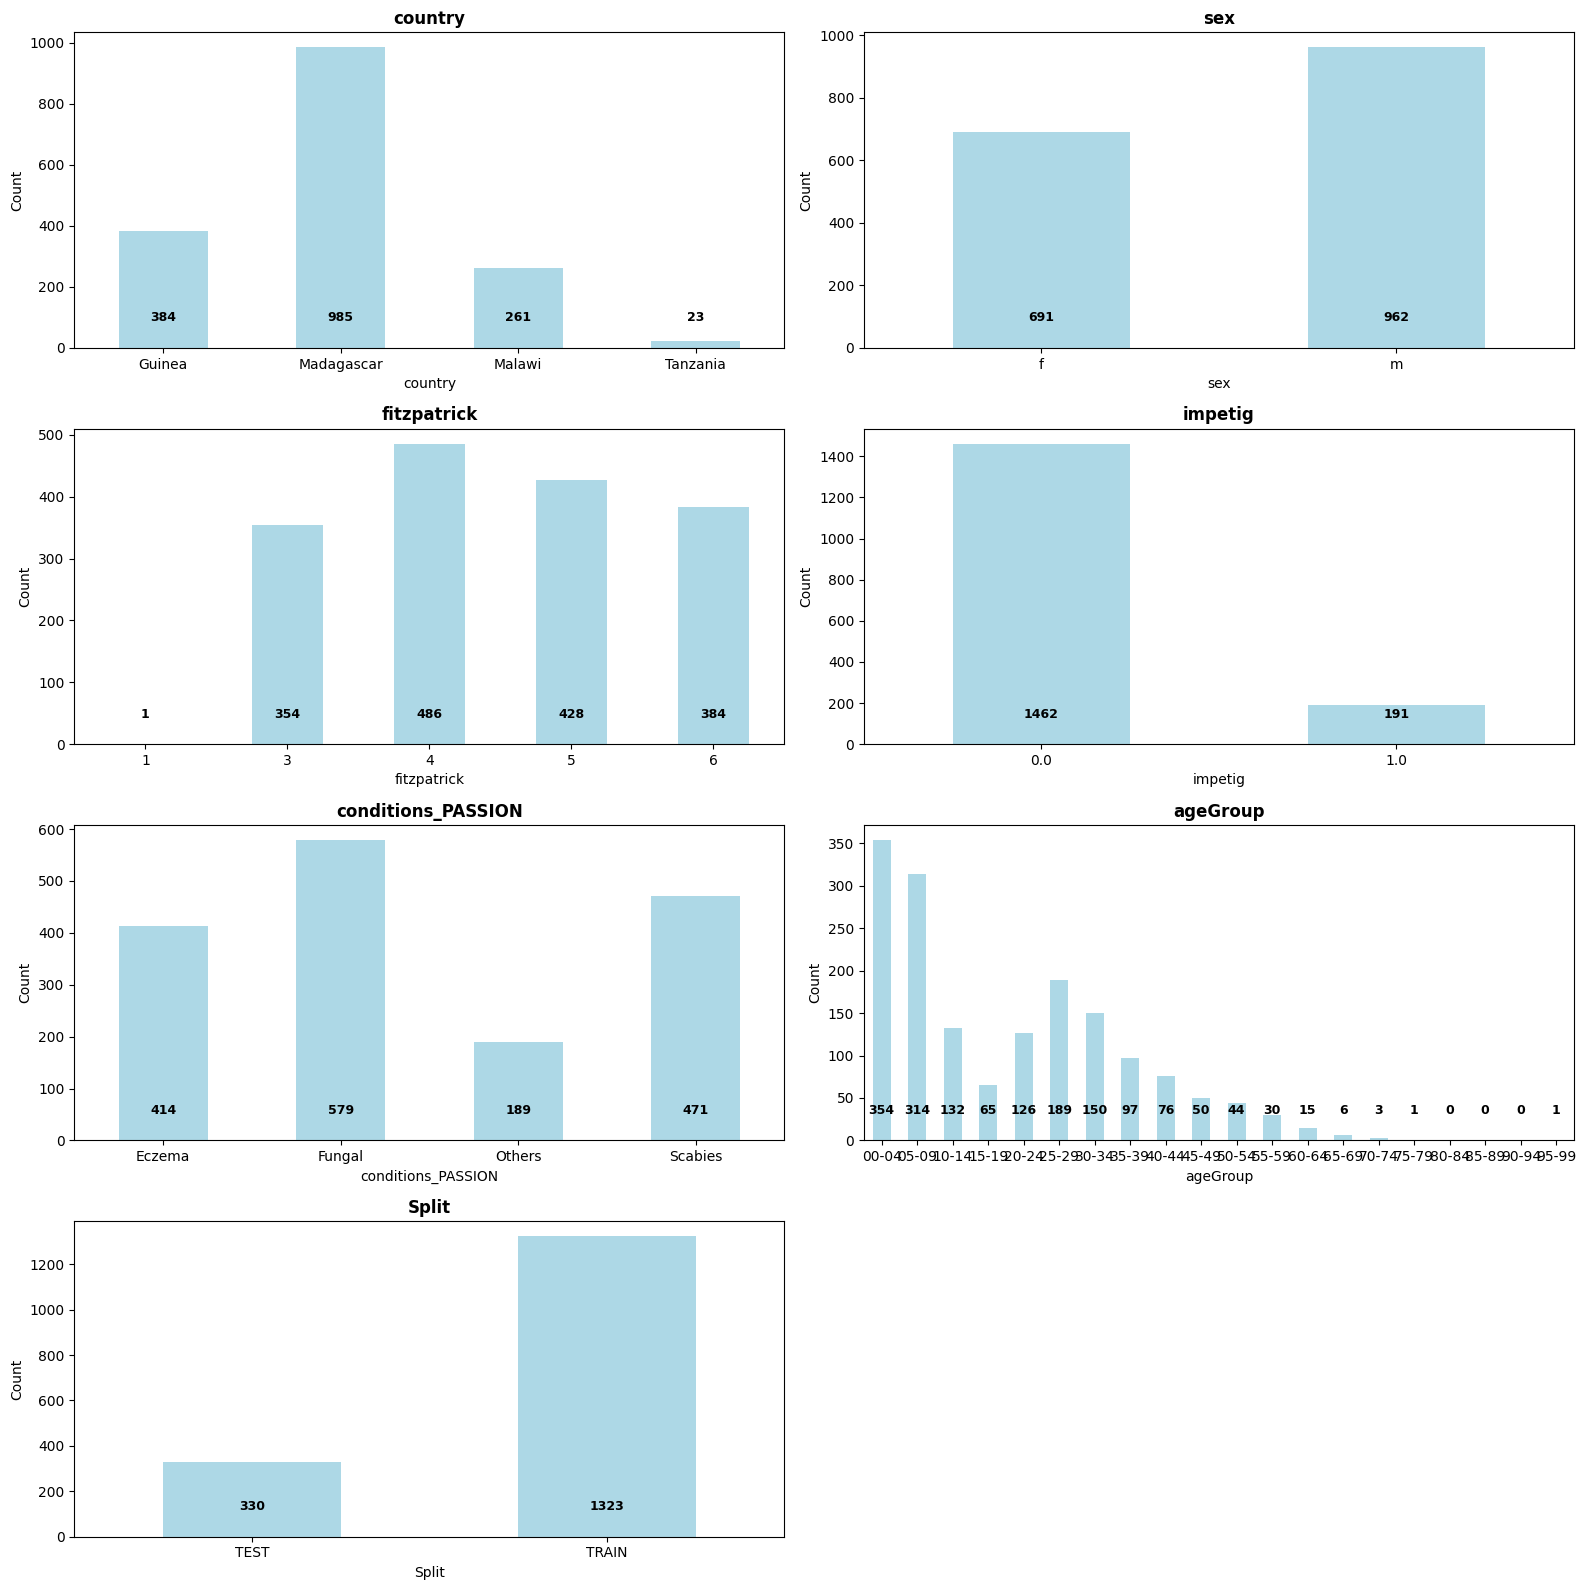
\includegraphics[width=0.9\textwidth]{figures/PASSION_split_all_distributions.png}
				\caption{PASSION dataset distribution analysis on group level}
				\label{fig:PASSIONDatasetDistrAnalysis}
			\end{figure}
			
			\begin{table}[H]
				\centering
				{
					\catcode`\_=12
					\csvautobooktabular{csvs/distribution_PASSION_split.csv}
					\catcode`\_=8
				}
				\caption{Distribution of metadata attributes in the PASSION dataset}
				\label{tbl:PASSIONDatasetDistrAnalysis}
			\end{table}
		\end{appendices}
		
		
		
			
		\glsaddallunused                                % add all unused items to glossary
		\todo{check the gls all unused.}
		
	
\end{document}
